\documentclass{book}



\usepackage{float}
\usepackage{amsmath}
\usepackage{amsfonts}
\usepackage{graphicx}
\usepackage{lineno}
\usepackage{natbib}
\usepackage{hyperref}
\usepackage{verbatim}
\usepackage{soul}
\usepackage{color}
\usepackage{bm}

\bibliographystyle{asa}

\floatstyle{plain}
\floatname{panel}{Panel}
\newfloat{algorithm}{h}{txt}[chapter]
\newfloat{panel}{h}{txt}[chapter]


\newcommand{\R}{\textbf{R}}
\newcommand{\bugs}{\textbf{BUGS}}
\newcommand{\jags}{\textbf{JAGS}}
\newcommand{\secr}{\mbox{\tt secr}}
\newcommand{\scrbook}{\mbox{\tt scrbook}}


\linenumbers

\begin{document}


\begin{comment}

\chapter{Introduction}
\label{chapt.intro}

\chapter{GLMS and WinBUGS}
\label{chapt.glms}
\end{comment}

\chapter{
 Closed Population Models
}
\markboth{Closed Population Capture-Recapture Models}{}
\label{chapt.closed}


\begin{comment}
XXXXXXXXXXXXXXXXXXXXXXXXXXXX
XXXXXXXXXXXXXXXXXXXXXXXXXXXX
- put posterior summaries in actual tables
- condense some of the DA material, it is a bit redundant and long
- use the same table structure (perhaps with hline at top and bottom)
- For the Bayesian analysis of model Mh where you find high prior 
sensitivity, perhaps investigate if the likelihood surface is flat, 
which would indicate that the problem is one affecting both classical 
and Bayesian analyses.
XXXXXXXXXXXXXXXXXXXXXXXXXXXXXXXXXXXXX
XXXXXXXXXXXXXXXXXXXXXXXXXXXXXXXXXXXXXXXX
\end{comment}


\vspace{.3in}

In this chapter we introduce  ordinary {\it non-spatial} capture-recapture (CR)
models for estimating population size in closed populations. A closed
population is one whose abundance $N$ does not change during the
study. Two forms of closure are often discussed: demographic closure,
meaning that no births or deaths occur, and geographic closure, which
states that no individuals move onto or off of the sampled area during the study.
Few populations are actually closed except during very short
time intervals, but closed population CR models serve as the basis for
the development of the rest of the models presented in this book,
including the models for open populations discussed in
Chapt.\ref{chapt.open}.

We will see that classical closed population CR models are closely
related to binomial (or logistic) regression-type models. In fact,
when $N$ is known, they are precisely logistic regression models.  We
consider some important extensions of ordinary closed population
models that accommodate various types of ``individual effects'' ---
either in the form of explicit, observed covariates (sex, age, body
mass) or unstructured ``heterogeneity'' in the form of an individual
random effect, which represent effects of unobserved or unmeasured
covariates. In general, these models are variations of generalized
linear or generalized linear mixed models (GLMs and GLMMs,
respectively).  Because of the paramount importance of this concept,
we focus mainly on fairly simple models in which the observations are
individual encounter frequencies, $y_{i}$ = the number of encounters
of individual $i$ out of $K$ replicate samples of the population
which, for the models we consider here, is the outcome of a binomial
random variable.
We begin with the most basic
capture-recapture model, colloquially referred to as ``model $M_0$''
\citep{otis_etal:1978}, in which encounter probability is strictly
constant in all respects (across individuals, and replicates).
 We then
consider extensions of that model to include individual heterogeneity
and individual covariates. A special type of individual covariate
models is distance sampling, which could be thought of as the most
primitive spatial capture-recapture model. 
In this chapter, we hope 
to establish the methodological linkage between non-spatial
and spatial capture-recapture models which we formalize in the next chapter.
 Along the way, 
we review some of
the informal methods of estimating density using CR methods, and
consider some of their limitations.  

%We will be exposed to our first
%primitive spatial capture-recapture models which arise as relatively
%minor variations of so-called ``individual covariate models'' (of the
%\citet{huggins:1989} and \citet{alho:1990} variety). 

We emphasize Bayesian analysis of capture-recapture models and we
accomplish this using a method related to classical ``data
augmentation'' from the statistics literature
\citep[e.g.,][]{tanner_wong:1987}.  This is a general concept in
statistics but, in the context of capture-recapture models where $N$
is unknown, it has a consistent implementation across classes of
capture-recapture models and one that is really convenient from the
standpoint of doing MCMC \citep{royle_etal:2007,royle_dorazio:2012}. We use data
augmentation throughout this book and thus emphasize its conceptual
and technical origins and demonstrate applications to closed
population models.  We refer the reader to
\citet[][ch. 6]{kery_schaub:2011} for an accessible and complementary
development of Bayesian analysis of ordinary, i.e., nonspatial closed population models.


\section{The Simplest Closed Population Model: Model $M_0$}

To start looking at the simplest capture-recapture model, let's suppose
there exists a population of $N$ individuals which we
subject to repeated sampling, say over $K$ ``occasions'', such as trap nights, where individuals
are captured, marked, released, and subsequently recaptured.  We suppose that
individual encounter histories are obtained, and these are of the form
of a sequence of 0's and 1's indicating capture $(y=1)$ or not $(y=0)$
during any sampling occasion.% XXX (``sample'') I prefer occasion since a
                            % sample could be spatial
As an example, suppose
$K=5$ sampling occasions, then an individual captured during occasion 
2 and 3 but not otherwise would have an encounter history of the form
${\bf y}=(0,1,1,0,0)$. Thus, the observation ${\bf y}_{i}$ for each
individual $(i=1,2,\hdots,N)$ is a vector having elements denoted by $y_{ik}$ for
$k=1,2,\hdots,K$. Usually this is organized as a row of a matrix with
elements $y_{ik}$, see Table \ref{closed.tab.3.1}. Except where noted
explicitly, we suppose that observations are independent within
individuals and among individuals.  Formally, this allows us to say
that $y_{ik}$ are independent and identically distributed (``$iid$'')
Bernoulli random variables and we may write $y_{ik}
\sim \mbox{Bern}(p)$.  Consequently, for this very simple model in
which $p$ is constant (i.e., there are no individual or temporal
covariates that affect $p$) the original binary detection variables
can be aggregated into total encounter frequencies for each individual
(total number of captures), $y_{i} = \sum_{k} y_{ik}$, and the
observation model changes from a Bernoulli distribution to a
binomial distribution based on a sample of size $K$. That is
\[
y_{i}  = \sum_{k} y_{ik} \sim \mbox{Binomial}(p,K)
\]
for every individual in the population $i=1,2,\ldots,N$, where $N$ is
the number of individuals in the population (i.e., population size).

We emphasize the central importance of the basic Bernoulli encounter model
-- an individual is either encountered in a sample, or not --
 which forms
the cornerstone of almost all of classical
capture-recapture models, including many spatial capture-recapture
models discussed in this book.

Evidently, the basic capture-recapture model is a simplistic version
of a logistic-regression model with only an intercept term
($\mbox{logit}(p) = \mbox{constant}$).  To say that all
capture-recapture models are just logistic regressions is only
slightly inaccurate. In fact, we are proceeding here as if we knew
$N$.  In practice we don't, of course, and estimating $N$ is actually
the central objective.  But, by proceeding as if $N$ were known, we
can specify a simple model and then deal with the fact that $N$ is
unknown using standard methods that you are already familiar with
(i.e., GLMs - see Chapt. \ref{chapt.glms}).
\begin{table}[ht]
\centering
\caption{A toy capture-recapture data set with $n=6$ observed
  individuals and $K=5$ sample occasions. Under a model with constant encounter
  probability, the binary detection history data can be summarized in the detection frequency (the total number of detections, $y_i$), which is shown in the right-most column.
}
\begin{tabular}{r|ccccc|c}
\hline
&  \multicolumn{5}{c}{Sample occasion} &  \\ \hline
 indiv $i$ &  1 & 2 & 3 & 4 & 5 & $y_{i}$ \\ \hline
  1 &     1 & 0 & 0 & 1 & 0  & 2   \\
  2 &     0 & 1 & 0 & 0 & 1  & 2   \\
  3 &     1 & 0 & 0 & 1 & 0  & 2   \\
  4 &     1 & 0 & 1 & 0 & 1  & 3   \\
  5 &     0 & 1 & 0 & 0 & 0  & 1   \\
  $n=6$ & 1 & 0 & 0 & 0 & 0  & 1   \\ \hline
\end{tabular}
\label{closed.tab.3.1}
\end{table}


Assuming individuals in the population are observed independently, the
joint probability distribution of the observations is the product of
$N$ binomials
\begin{equation}
  \Pr(y_1, \ldots, y_N | p) = \prod_{i=1}^N  \mathrm{Binomial}(y_i | K, p).
  \label{closed.eq.binNknown}
\end{equation}
We emphasize that this expression is conditional on $N$, in which
case we get to observe the $y_i=0$ observations and the resulting data
are just $iid$ binomial counts. Because this is a binomial regression
model of the variety described in Chapt. \ref{chapt.glms}, fitting this model using
a {\bf BUGS} engine poses no difficulty.

Equation~\ref{closed.eq.binNknown} can be simplified even further if we reformat the
observations as capture frequencies, which are the sufficient
statistics under this model. Specifically, let $n_k$ denote the number
of individuals captured exactly $k$ times after $K$ survey occasions, $n_k = \sum_{i=1}^N
I(y_i = k)$ where $I$ is the indicator function evaluating to 1 if its
argument is true and 0 otherwise. For sake of illustration,
we converted the data from Table~\ref{closed.tab.3.1} to this
format (Table~\ref{closed.tab.3.1.nk}). What is important to note is
that if we know $N$, then we known $n_0$, i.e. the number of
individuals not captured at all. In this case, an alternative and equivalent expression to
Eq.~\ref{closed.eq.binNknown} is
\begin{equation}
  \Pr(y_1, \ldots, y_N | p) = \prod_{k=0}^K  \pi_{k}^{n_k}
  \label{closed.eq.multiNknown}
\end{equation}
where $\pi_{k} = \mathrm{Pr}(y=k)$ under the binomial model with
parameter $p$ and sample size $K$. 

\begin{table}[ht]
\centering
\caption{Data from Table~\ref{closed.tab.3.1} formatted as capture
  frequencies. Since $N$ is unknown, the number of individuals not
  captured ($n_0$) is also unknown.}
\begin{tabular}{lcccccc}
\hline
& \multicolumn{6}{c}{$k$} \\
\cline{2-7}
 & 0  & 1 & 2 & 3 & 4 & 5 \\
\hline
Number of individuals captured $k$ times ($n_k$) & $N\; - \; 6$ & 2 & 3 & 1 & 0 & 0 \\
\hline
\end{tabular}
\label{closed.tab.3.1.nk}
\end{table}

The essential problem in capture-recapture, however, is that $N$ is
{\it not} known because the number of uncaptured 
individuals ($n_0$)
%(i.e., those in the zero cell that occur with probability $\pi_0$)
is unknown. % I added some text here, which is kind of clunky but this
            % section was moving too fast I think.
Consequently, the observed capture frequencies $n_k$ are no
longer independent because $n_0$ is a function of the other
frequencies, $n_0 = N-\sum_{k=1}^K n_k$. Hence, their joint distribution is multinomial
(e.g., see \citet[][p. 61]{illian_etal:2008}):
%\hl{Andy, I changed this from n_1, n_2 to n_0, n_1. Isn't that right?}
\begin{equation}
    n_0, n_1, \ldots, n_K \sim \mathrm{Multinomial}(N, \pi_0, \pi_1, \ldots, \pi_K)
\label{closed.eq.multinomial4m0}
\end{equation}
We give a general overview of the multinomial distribution in
Sec. \ref{sec.modeling.distributions}. The multinomial distribution is
the standard model for discrete responses that can fall into a fixed
number ($K+1$ in this case) of possible categories. In the context of
capture-recapture, the multinomial posits a population of $N$
individuals with $K+1$ possible outcomes defined by the possible
encounter frequencies: captured $y=1,2,\ldots,K$ times or not captured
at all. These possible outcomes occur with
probabilities $\pi_{k}$, which we refer to as ``cell probabilities''
or in the specific context of capture-recapture, encounter history
probabilities.
%We denote the number of uncaptured/missing individuals
%by $n_0$, and the total number of distinct individuals encountered in
%the $K$ samples by $n = \sum_{k=1}^K n_k$.  Note that $n_{0}$ appears
%in the likelihood as a component of $N = n + n_{0}$.


To fit the model in which $N$ is {\it unknown}, we can regard $n_{0}$ as a
parameter and maximize the multinomial likelihood directly.
Direct likelihood analysis of the multinomial model is
straightforward, but that is not always sufficiently useful in practice
because we seldom are concerned with models for the aggregated
encounter history frequencies, which entail that capture probabilities are the
same for all individuals. In many instances, including for
spatial capture-recapture (SCR) models, we require a formulation of
the model that can accommodate individual-level
covariates to account for
differences in detection among individuals which we
address subsequently in this chapter and also in Chapt. \ref{chapt.covariates}.



\begin{comment}
\subsection{The Spatial Context of Capture-Recapture}

XXX I WOULD CHANGE THE SECTION HEADING TO SOMETHING LIKE 'POPULATION CLOSURE AND THE SPATIAL
CONTEXT OF CAPTURE-RECAPTURE XXX

A common assumption made is that of population ``closure'' which is
really just a colloquial way of saying (in part) the Bernoulli
assumptions stated explicitly above. In the biological context,
closure means, strictly, no additions or subtractions from the
population during study. This is manifest by the statement that the
encounters are independent and identically distributed (iid) Bernoulli
trials.  In practice, closure is usually interpreted by the manner in
which potential violations of that assumption arise. In particular,
two important elements of the closure assumption are ``demographic''
and ``geographic'' closure. If an individual dies then subsequent
values of $y_{ik}$ are clearly no longer Bernoulli trials with the
same parameter $p$; since the probability of capturing that individual becomes 0. If there is no mortality or recruitment in the
population, then we say that demographic closure is
satisfied. Similarly, animals may emigrate or immigrate. If they do
not, then geographic closure is satisfied. Sometimes a distinction is
made between temporary and permanent emigration or immigration. That
is a relevant distinction in spatial capture-recapture models, because
SCR models explicitly accommodate ``temporary emigration'' of a
certain type, due to individuals moving about their home range.
In contrast, ordinary capture-recapture models cannot explicitly deal
with the fact that, unless we're sampling a fenced enclosure or an
island, individuals are bound to move ``off the trapping grid''
(whatever that means).  The
demographic closure assumption can also be relaxed using SCR models,
but we will save that discussion for Chapt. \ref{chapt.scr0}.

XXXX I FEEL LIKE THIS SECTION STILL NEEDS A SENTENCE THAT MAKES THE POINT - SPATIAL CONTEXT; POP CLOSURE AND SCR;
BUT I AM HAVING TROUBLE PUTTING THAT INTO A FEW WORDS RIGHT NOW XXXX

\end{comment}

\subsection{The Core Capture-Recapture Assumptions}

This  basic capture-recapture model -- model $M_{0}$ -- comes with it
a host of specific biological and statistical assumptions.
In addition to the basic assumption of population closure,
\citet{otis_etal:1978} list the following:
\begin{enumerate}
  \item animals do not lose their marks during the experiment,
  \item all marks are correctly noted and recorded at each trapping
    occasion, and
  \item each animal has a constant and equal probability of capture on
    each trapping occasion.
\end{enumerate}
The remainder of their classic work is dedicated to relaxing
assumption 3. While assumptions 1 and 2 are undoubtedly necessary for
inference from basic CR methods to be valid, and while they are
also assumed by most of the models we present in the following
chapters, we refrain from repeatedly making such statements. Our
opinion is that all model assumptions are apparent when a model is
clearly specified, and it is both redundant and impossible to list all
the things not allowed by the model. For example, closed population
models also assume that other sources of data entry do not occur, but
it is not necessary to enumerate each possibility. Rather, it is
necessary to make clear statements such as
\[
y_i \stackrel{iid}{\sim} \text{Bernoulli}(p) \quad \: \text{for}\: i=1,\ldots,N.
\]
This simple model description carries a tremendous amount of
information, and it leaves very little left to say with respect to
assumptions. Although we will not always show the $iid$ symbol, it
will be assumed unless otherwise noted, and this assumption is
critical for valid inference. It implies that the encounter of one
individual does not affect the encounter of another
individual. Under this assumption, it is  easy to write down the
likelihood of the parameters and obtain parameter estimates; however,
whether or not it is true depends upon biological and sampling
issues. If this assumption is deemed false, the model can be discarded
in favor of a more realistic alternative. However, once we have
settled on our model, statistical inference proceeds by assuming the
model is truth---not an approximation to truth---but actual
truth.
%; yet as with every model assumption ever made in the history of
%statistics, the core capture-recapture assumptions are not correct. This might
%come as a major shock to some people.

In spite of the fact that we assume that all models are truth, but we
acknowledge that all models are wrong due to their assumptions,
assumptions should not be viewed as a necessary evil. In fact, one way
to view assumptions is as embodiments of our ecological hypotheses. If
we make these assumptions too complex or too specific, then we will
never be able to study general phenomenon that hold true across space
and time. Furthermore, in practice, we will rarely have enough data to estimate the
parameters of highly complex models.



\begin{comment}
then there is not much more to say with respect to assumptions. For
example, if animals lost their marks, then clearly this statement would
not apply because we would not be able to know which individual we
encountered. The same is true concerning assumption 2---if marks are
not correctly recorded, then there is measurement error not accounted
for by our model.

The point of the above discussion is that all of the assumptions are
embodied in a clear statement of the model. More generally, %and this
%is a point not usually understood by people
%who use capture-recapture models, %is that
we assume that {\it the model is properly specified} which means everything that is {\it not}
in the model. In reality, there are infinite things not covered by the model, and
therefore we think being specific about what it {\it does} assume,
explicitly identified by the model, is preferred.



Encounter events of the same individual are independent of one
another. Usually this is not, but we can build models that contain
covariates.
Of course spatial location is a sensible covariate for encounter
probability and the whole point of SCR models is to induce a certain
type of non-independence as a result of individual location relative
to traps.
\end{comment}



\subsection{Conditional likelihood}

%%%%% xxxxx Drop that section title and simply go on explaining
%%%%% things. Replace title with a topical sentence: for instance, ?a
%%%%% typical analysis of this model is based on conditional
%%%%% likelihood (plus some references)?

We saw that the closed population model is a simple logistic
regression model if $N$ is known and, when $N$ is unknown, the model
is multinomial with index or sample size parameter $N$. This
multinomial model, being conditional on $N$, is sometimes referred to
as the ``joint likelihood'' the ``full likelihood'' or the
``unconditional likelihood'' (sometimes
``model'' in place of ``likelihood'')
\citep{sanathanan:1972,borchers_etal:2002}. This
formulation differs from the so-called ``conditional likelihood''
approach in which the likelihood of the observed encounter histories
is devised conditional on the event that an individual is captured at
least once.  To construct this likelihood, we have to recognize that
individuals appear or not in the sample based on the value of the
random variable $y_{i}$, that is, we capture them if and only if
$y_{i}>0$.  The observation model is therefore based on $\Pr(y|y>0)$.
For the simple case of model $M_0$, the resulting conditional
distribution is a ``zero truncated'' binomial distribution which
accounts for the fact that we cannot observe the value $y=0$ in the
data set. % \citep[see][sec. 5.1]{royle_dorazio:2008}. 
 Both the
conditional and unconditional models are legitimate modes of analysis
in all capture-recapture types of studies, and they provide equally
valid descriptions of the data and for many practical purposes provide
equivalent inferences, at least in large sample sizes
\citep{sanathanan:1972}.

In this book we emphasize Bayesian analysis of capture-recapture
models using data augmentation
(described in sec. \ref{closed.sec.da} below), which
produces yet a third distinct formulation of capture-recapture models
based on the zero-{\it inflated} binomial distribution that we
describe in the next section.  Thus, there are 3 distinct formulations
of the model -- or modes of analysis -- for analyzing all
capture-recapture models based on the (1) binomial model for the joint
or unconditional specification; (2) zero-truncated binomial that
arises ``conditional on $n$''; and (3) the zero-inflated binomial that
arises under data augmentation.  Each formulation has distinct
model parameters (shown in Table \ref{tab.3.modes} for
model $M_0$).


\begin{table}[ht]
\centering
\caption{Modes of analysis of capture-recapture models. Closed
  population models can be analyzed using the joint or ``full
  likelihood'' which contains $N$ as an explicit parameter, the
  conditional likelihood which does not involve $N$, or by data
  augmentation which replaces $N$ with $\psi$. Each approach yields a
  distinct likelihood.}
\begin{tabular}{ccc}
\hline \hline 
Mode of analysis & parameters in model & statistical model \\ \hline
Joint likelihood                &	$p$, $N$	&	multinomial with index $N$\\
Conditional likelihood 		&	$p$	&	zero-truncated binomial \\
Data augmentation		&	$p$, $\psi$	&
zero-inflated binomial\\
\hline
\end{tabular}
\label{tab.3.modes}
\end{table}



\section{Data Augmentation }
\label{closed.sec.da}

We consider a method of analyzing closed population models using
parameter-expanded data augmentation (PX-DA), which we abbreviate to
``data augmentation'' or DA, which is useful for Bayesian analysis
and, in particular, analysis of models using the various \bugs~engines
and other Bayesian model fitting software.  Data augmentation is a
general statistical concept that is widely used in statistics in many
different settings. The classical reference is
\citet{tanner_wong:1987}, but see also \citet{liu_wu:1999}.  Data
augmentation can be adapted to provide a very generic framework for
Bayesian analysis of capture-recapture models with unknown $N$. This
idea was introduced for closed populations by \citet{royle_etal:2007},
and has subsequently been applied to a number of different contexts
including individual covariate models \citep{royle:2009}, open
population models \citep{royle_dorazio:2008,royle_dorazio:2012,
  gardner_etal:2010ecol}, spatial capture-recapture models
\citep{royle_young:2008, royle_etal:2010, gardner_etal:2009}, and many
others. \citet[][Chapt. 6]{kery_schaub:2011} provides a good
introduction to data augmentation in the context of closed population
models.



Conceptually, the technique of data augmentation represents a
reparameterization of the ``complete data'' model -- i.e., that
conditional on $N$. The reparameterization is achieved by embedding
this data set into a larger data set having $M> N$ ``rows''
(individuals) and re-expressing the model conditional on $M$ instead
of $N$. The great thing about data augmentation is that we do not need
to know $N$ for this reparameterization.  Although this has a whiff of
arbitrariness or even outright ad hockery to it, in the choice of $M$,
it is always possible, in practice, to choose $M$ pretty easily for a
given problem and context and results will be insensitive to choice of
$M$\footnote{Unless the data set is sufficiently small that parameters
  are weakly identified}.  Then, under data augmentation, analysis is
focused on the ``augmented data set.'' That is, we analyze the bigger
data set - the one having $M$ rows - with an appropriate model that
accounts for the augmentation. This is achieved by a Bernoulli
sampling process that determines whether an individual in $M$ is also
a member of $N$.  Inference is focused directly on estimating the
proportion $\psi = E[N]/M$, instead of directly on $N$, where $\psi$
is the ``data augmentation parameter.''


\subsection{DA links occupancy models and closed population models}


There is a close correspondence between so-called ``occupancy'' models and closed
population models \citet[see][sec. 5.6]{royle_dorazio:2008}.
In occupancy models \citep{mackenzie_etal:2002, tyre_etal:2003} the
sampling situation is that $M$ sites, or patches, are sampled multiple
times to assess whether a species occurs at the sites.  This yields
encounter data such as that illustrated in the left panel of Table
\ref{closed.tab.occ}. The important problem is that a species may
occur at a site, but go undetected, yielding an all-zero encounter
history for the site, which in the case of occupancy studies, are {\it
  observed}. However, some of the zero vectors will typically correspond
to sites where the species in fact {\it does} occur. Thus, while the
zeros are observed, there are too many of them and, in a sense, the
inference problem is to partition the zeros into ``structural''
(fixed) and ``sampling'' (or stochastic) zeros, where the former are
associated with unoccupied and the latter with occupied sites where
the species went undetected. More
formally, inference is focused on the parameter $\psi$, the
probability that a site is occupied.

In contrast to occupancy studies, in classical closed
population studies, we observe a data set as in the middle panel of
Table \ref{closed.tab.occ} where {\it no} zeros are observed. The
inference problem is, essentially, to estimate how many sampling zeros
there are -- or should be -- in a ``complete'' data set. This objective
(how many sampling zeros?) is precisely the same for both types of
problems if an upper limit $M$ is specified for the closed population
model. The only distinction being that, in occupancy models, $M$ is
set by design (i.e., the number of sites in the sample), whereas a natural
choice of $M$ for capture-recapture models may not be
obvious. However, the choice of $M$ induces a uniform prior for $N$ on
the integers $[0,M]$ \citep{royle_etal:2007}. Then, one can analyze
capture-recapture models by adding $M-n$ all-zero encounter histories
to the data set and regarding the augmented data set, essentially, as
a site-occupancy data set, where the occupancy or data augmentation parameter ($\psi$) takes
the place of the abundance parameter ($N$).

Thus, the heuristic motivation of data augmentation is to fix the size
of the data set by adding {\it too many} all-zero encounter histories
to create the data set shown in the right panel of Table
\ref{closed.tab.occ}, and then analyze the augmented data set using an
occupancy type model which includes both ``unoccupied sites'' (in
capture-recapture, augmented individuals that are not members of the
real population that was sampled) as well
as ``occupied sites'' (in capture-recapture, individuals that are
members of the population but that were undetected by sampling) at which detections did not occur. We call these
$M-n$ all-zero histories ``potential individuals'' because they exist
to be recruited (in a non-biological sense) into the population, for
example during an analysis by MCMC.

To analyze the augmented data set, we recognize that it is a
zero-inflated version of the known-$N$ data set. That is, some of the
augmented all-zero rows are sampling zeros (corresponding to actual
individuals that were missed) and some are ``structural'' zeros, which
do not correspond to individuals in the population. For a basic
closed-population model, the resulting likelihood under data
augmentation - that is, for the data set of size $M$ -- is a simple
zero-inflated binomial likelihood.  The zero-inflated binomial model
can be described ``hierarchically'', by introducing a set of binary
latent variables, $z_{1},z_{2},\ldots, z_{M}$, to indicate whether
each individual $i$ is ($z_i=1$) or is not ($z_i=0$) a member of the
population of $N$ individuals exposed to sampling. We assume that
$z_{i} \sim \mbox{Bernoulli}(\psi)$ where $\psi$ is the probability that an
individual in the data set of size $M$ is a member of the sampled
population -- in the sense that $1-\psi$ is the probability of
realizing a ``structural zero'' in the augmented data set.  The
zero-inflated binomial model which arises under data augmentation can
be formally expressed by the following set of assumptions (we include
typical priors for a Bayesian analysis):
\begin{eqnarray*}
 y_{i}|{z_{i}=1} & \sim  &\mbox{Binomial}(K, p) \\
 y_{i}|{z_{i}=0} & \sim &  1(y=0)  \\
 z_{i} & \stackrel{iid}{\sim} & \mbox{Bernoulli}(\psi) \\
 \psi & \sim & \mathrm{Uniform}(0,1) \\
 p & \sim & \mathrm{Uniform}(0,1)
\end{eqnarray*}
for $i=1, \ldots, M$, where $1(y=0)$ is a point mass at
$y=0$.
It is sometimes convenient to express the conditional-on-$z$
observation model concisely in
just one step:
\[
 y_{i}|z_{i}  \sim  \mbox{Binomial}(K, z_{i} p) \\
\]
and we understand this to mean, if $z_{i}=0$, then $y_{i}$ is
necessarily 0 because its success probability is $z_{i} p = 0$.

Note that, under data augmentation, $N$ is no longer an explicit
parameter of this model. In its place, we estimate $\psi$ and
functions of the latent variables $z$. In particular, under the
assumptions of the zero-inflated model, $z_{i} \stackrel{iid}{\sim}
\mbox{Bern}(\psi)$; therefore, $N$ is a function of these latent
variables:
 \[
 N = \sum_{i=1}^{M} z_{i}.
\]
Further, we note that the latent $z_i$ parameters {\it can be} removed
 from
the model by integration, in which case the joint probability of the
data is
\begin{equation}
  \Pr(y_1, \ldots, y_M | p, \psi) = \prod_{i=1}^M  \psi \mathrm{Binomial}(y_i | K, p) +  I(y_i=0) (1-\psi)
\end{equation}
Interpreted as a likelihood, we can directly maximize this expression
to obtain the MLEs of the structural parameters $\psi$ and $p$ or
those of other more complex models \citep[e.g., see][]{royle:2006}. We
could estimate these parameters and then use them to obtain an
estimator of $N$ using the so-called ``Best unbiased predictor''
\citep[see][]{royle_dorazio:2012}. Normally, however, we will analyze
the model in its ``conditional-on-$z$'' form using methods of MCMC
either in the {\bf BUGS} engines or using our own MCMC algorithms (see
Chapt. \ref{chapt.mcmc}).

\begin{table}[ht]
\centering
\caption{Hypothetical occupancy data set (left), capture-recapture data
 in standard form (center), and capture-recapture data augmented with
 all-zero capture histories (right). }
\begin{tabular}{cccc|cccc|cccc}
\hline
\multicolumn{4}{c}{Occupancy data}    &
\multicolumn{4}{c}{Capture-recapture} &
\multicolumn{4}{c}{Augmented C-R}     \\ \hline
site    & k=1 & k=2 & k=3 & ind & k=1 &k=2  & k=3 & ind & k=1 & k=2 & k=3           \\ \hline
1  & 0   & 1   & 0   & 1   & 0   & 1  & 0   & 1   & 0   & 1   & 0                   \\
2  & 1   & 0   & 1   & 2   & 1   & 0 & 1    & 2 & 1 & 0 & 1 \\
3  & 0   & 1   & 0   & .   & 0   & 1 & 0    & 3 & 1 & 0 & 1 \\
4  & 1   & 0   & 1   & .   & 1   & 0 & 1    & 4 & 1 & 0 & 1 \\
5  & 0   & 1   & 1   & .   & 0   & 1 & 1    & 5 & 1 & 0 & 1 \\
.  & 0   & 1   & 1   & .   & 0   & 1 & 1    & . & 0 & 1 & 1 \\
.  & 1   & 1   & 1   & .   & 1   & 1 & 1    & . & 0 & 1 & 1 \\
.  & 1   & 1   & 1   & .   & 1   & 1 & 1    & . & 1 & 1 & 1 \\
   & 1   & 1   & 1   & .   & 1   & 1 & 1    & . & 1 & 1 & 1 \\
n  & 1   & 1   & 1   & n   & 1   & 1 & 1    & n & 1 & 1 & 1 \\
.  & 0   & 0   & 0   &     &     &   &      & . & 0 & 0 & 0 \\
.  & 0   & 0   & 0   &     &     &   &      & . & 0 & 0 & 0 \\
   & 0   & 0   & 0   &     &     &   &      &   & 0 & 0 & 0 \\
   & 0   & 0   & 0   &     &     &   &      &   & 0 & 0 & 0 \\
   & 0   & 0   & 0   &     &     &   &      &   & 0 & 0 & 0 \\
   & 0   & 0   & 0   &     &     &   &      & N & 0 & 0 & 0 \\
.  & 0   & 0   & 0   &     &     &   &      & . & 0 & 0 & 0 \\
.  & 0   & 0   & 0   &     &     &   &      &   & 0 & 0 & 0 \\
M  & 0   & 0   & 0   &     &     &   &      & . & 0 & 0 & 0 \\
   &     &     &     &     &     &   &      & . & . & . & . \\
   &     &     &     &     &     &   &      & . & . & . & . \\
   &     &     &     &     &     &   &      & . & . & . & . \\
   &     &     &     &     &     &   &      & M & 0 & 0 & 0 \\
\hline
\end{tabular}
\label{closed.tab.occ}
\end{table}


\subsection{Model $M_0$ in BUGS}

It is helpful to understand data augmentation by seeing what its
effect is on implementing model $M_0$. For this model, 
 in which we can aggregate the encounter data to
individual-specific encounter frequencies, the augmented data are
given by the vector of frequencies $(y_{1}, \ldots, y_{n}, 0, 0,
\ldots, 0)$ where the augmented values of $y=0$ represent the encounter
frequency  for pseudo-individuals $y_{n+1},\ldots,y_{M}$.
The zero-inflated model of the augmented data combines
the model of the latent variables, $z_{i} \sim \mbox{Bern}(\psi)$ with
the conditional-on-$z$ binomial model:
\[
y_{i}|z_{i}   \sim \mbox{Binomial}(K,z_{i} p)
\]
so that, if $z_{i}=0$, the success probability of the binomial
distribution is identically 0 whereas, if $z_{i}=1$, the success
probability is $p$. This is useful in describing the model in the {\bf
  BUGS} language, as shown in Panel \ref{closed.panel.da4m0}.
 Note the last line of the model
specification  provides the expression for computing $N$ from the
data augmentation variables $z_{i}$. Note that, to improve readability of code
snippets (especially of large ones), we will sometimes deviate from our
standard notation a bit. In this case we use \mbox{\tt nind} for $n$
(the number of encountered individuals), and \mbox{\tt M = nind + nz}
is the total size of the augmented data set. In other cases we might
also use \mbox{\tt nperiods} in place of $K$ and \mbox{\tt ntraps} in
place of $J$. We find that word definitions make code easier to
understand, especially without having to read surrounding text.

\begin{panel}[ht]
\centering
\rule[0.15in]{\textwidth}{.03in}
%\begin{minipage}{5in}
{\small
\begin{verbatim}
model{
p  ~ dunif(0,1)
psi~dunif(0,1)

# nind = number of individuals captured at least once
#   nz = number of uncaptured individuals added for DA
for(i in 1:(nind+nz)) {
    z[i]~dbern(psi)
   mu[i]<-z[i]*p
    y[i]~dbin(mu[i],K)
 }

N<-sum(z[1:(nind+nz)])
}
\end{verbatim}
}
%\end{minipage}
\rule[-0.15in]{\textwidth}{.03in}
\caption{Model $M_{0}$ under data augmentation. Here \mbox{\tt y},
  \mbox{\tt K}, \mbox{\tt n} and \mbox{\tt nz} are provided as
  data. The population size parameter $N$ is computed as a function of
the data augmentation variables $z$. }
\label{closed.panel.da4m0}
\end{panel}





Specification of a more general model in terms of the individual
encounter observations $y_{ik}$ is not much more difficult than for
the individual encounter frequencies.  We define the
observation model by a double loop and change the indexing of quantities
accordingly, i.e.,
{\small
\begin{verbatim}
for(i in 1:(nind+nz)) {
    z[i]~dbern(psi)
  for(k in 1:K){
      mu[i,k]<-z[i]*p
      y[i,k]~dbin(mu[i,k],1)
  }
}
\end{verbatim}
}
In this manner, it is straightforward to incorporate covariates on $p$
for both individuals and sampling occasions
(see discussion of this below and also Chapt. \ref{chapt.covariates})
as well as to devise other extensions of the model, including models
for open populations (see Chapt. \ref{chapt.open}).

\subsection{Formal development of data augmentation (DA) }

Use of parameter-expanded data augmentation (PX-DA), or DA for short, for solving inference problems with unknown $N$ can be
justified as originating from the choice of a uniform prior on $N$.  The
$\mathrm{Uniform}(0,M)$ prior for $N$ is innocuous in the sense that the
posterior associated with this prior is equal to the likelihood for
sufficiently large $M$.  One way of inducing the $\mathrm{Uniform}(0,M)$
prior on $N$ is by assuming the following hierarchical prior:
\begin{eqnarray}
\label{closed.eq.NgivenM}
  N &\sim& \mathrm{Binomial}(M, \psi) \\ \nonumber
  \psi &\sim& \mathrm{Uniform}(0,1)
\end{eqnarray}
which includes a new model parameter $\psi$
(note that we have seen $\psi$ in the previous section as the proportion $E[N]/M$).
This parameter denotes
the probability that an individual in the super-population of size $M$
is a member of the population of $N$ individuals exposed to sampling.
The model assumptions, specifically the multinomial model
(Eq. \ref{closed.eq.multinomial4m0})
and Eq. \ref{closed.eq.NgivenM}, may be combined to yield a
reparameterization of the conventional model that is appropriate for
the augmented data set of known size $M$:
\begin{equation}
\label{closed.eq.multinomial4DA}
    (n_1, n_2, \ldots, n_K) \sim \mathrm{Multinomial}(M, \psi  \pi_{1}, \psi \pi_{2}, \ldots, \psi \pi_{K})
\end{equation}
This expression arises by removing $N$ from Eq. \ref{closed.eq.multinomial4m0} by
integrating
over the binomial prior distribution for $N$. Thus, the models we
analyze under data augmentation arise formally by removing the
parameter $N$ from the ordinary closed-population model---the model
conditional on $N$---by integrating over a binomial prior distribution
for $N$.

Note that the $M-n$ unobserved individuals in the augmented data set
have probability $\psi \pi(0) + (1-\psi)$, indicating that these
unobserved individuals are a mixture of individuals that are sampling
zeros ($\psi \pi_0$), and belong to the population of size $N$, and
others that are ``structural zeros'' (occurring in the augmented data
set with probability $1 - \psi$). In Eq.~\ref{closed.eq.multinomial4DA} $N$
has been eliminated as a formal parameter of the model by
marginalization (integration) and replaced with the new parameter
$\psi$, the data augmentation parameter.
However, the full likelihood containing both $N$ and $\psi$ can also be
analyzed \citep[see][]{royle_etal:2007}.


\subsection{Remarks on Data Augmentation}
\label{closed.sec.remarks}

Data augmentation may seem like a strange and mysterious black-box,
and likely it is unfamiliar to most people, even to many of those with substantial
experience with capture-recapture models. However, it really is just a
formal reparameterization of capture-recapture models in which $N$ is
marginalized out of the ordinary (conditional-on-$N$) model (by summation).
%In the case of model $M_0$, data augmentation produces the zero-inflated
%binomial which is distinct from the original model, but
%only in the sense that it embodies, explicitly, the $\mbox{Unif}(0,M)$
%prior for $N$.  
As a result, we could refer to the resulting model as the 
``binomial-integrated likelihood'' to reflect that an estimator could
be obtained from the ordinary likelihood, integrated over a binomial
prior. Other such ``integrated likelihood'' models are sensible. For
example, we could place a Poisson prior on $N$ with mean $\Lambda$ and
marginalize $N$ over the Poisson prior. This produces a likelihood in
which $\Lambda$ replaces $N$, instead of $\psi$ replacing $N$.  We
note that this type of marginalization over a Poisson prior is what
the {\bf R} package \mbox{\tt secr} does in its analysis of spatial
capture-recapture models (see Sec. \ref{mle.sec.secrguts}).


We emphasize the motivation for data augmentation being that it
produces a data set of fixed size, so that the parameter dimension in
any capture-recapture model is also fixed.  As a result, MCMC is a
relatively simple proposition using standard Gibbs Sampling.  And, in
particular, capture-recapture models become trivial to implement in
{\bf BUGS}. Consider the simplest context---analyzing model $M_0$
using the occupancy-type model. In this case, DA converts model $M_0$
to a basic occupancy model and the parameters $p$ and $\psi$ have
known full-conditional distributions (in fact, beta distributions)
that can be sampled from directly.  Furthermore, the data augmentation
variables, i.e., the collection of $z$'s, can be sampled from
Bernoulli full conditionals. MCMC is not much more difficult for
complicated models---sometimes the hyperparameters need to be sampled
using a Metropolis-Hastings step (e.g., Chapt. \ref{chapt.mcmc}), but
nothing more sophisticated than that is required.

Potential sensitivity of parameter estimates (especially of $N$) might
be cause for some concern.
The guiding principle is
that it should be chosen large enough so that the posterior for $N$ is
not truncated, but it should not be too large due to the increased 
computational burden. It seems likely that the properties of the
Markov chains should be affected by $M$ and so some optimal choice of
$M$ might exist \citep{gopalaswamy:2012}.
Formal analysis of this is needed.

There are other approaches to analyzing models with unknown $N$, using
reversible jump MCMC (RJMCMC) or other so-called ``trans-dimensional''
(TD) algorithms \citep{king_brooks:2001, durban_elston:2005,
  king_etal:2008, schofield_barker:2008, wright_etal:2009}.  What
distinguishes DA from RJMCMC and related TD methods is that DA is used
to create a distinctly new model that is unconditional on $N$ and we
(usually) analyze the unconditional model. The various TD/RJMCMC
approaches seek to analyze the conditional-on-$N$ model in which the
dimension of the parameter space is a function of $N$, and will
therefore typically vary at each iteration of the MCMC
algorithm. TD/RJMCMC approaches might appear to have the advantage
that one can model $N$ explicitly or consider alternative priors for
$N$. However, despite that $N$ is removed as an explicit parameter in
DA, it is possible to develop hierarchical models that involve
structure on $N$ \citep{converse_royle:2012, royle_etal:2012arXiv} which
we consider in Chapt. \ref{chapt.hscr}. Furthermore, data augmentation
is often easier to implement than RJMCMC and the details of the
DA implementation are the same for all capture-recapture problems.


\subsection{Example: Black Bear Study on Fort Drum}

To illustrate the analysis of model $M_0$ using data augmentation, we use
a data set collected at Fort Drum Military Installation in upstate New
York by P.D. Curtis and M.T Wegan of Cornell University and
their colleagues at the Fort Drum Military Installation.
These data have been analyzed in various forms by
\citet{wegan:2008,gardner_etal:2009} and \citet{gardner_etal:2010jwm}.
The specific data used here are encounter histories on 47 individuals
obtained from an array of 38 baited ``hair snares''
(Fig. \ref{closed.fig.fortdrum}) during June and July 2006.  Barbed wire
traps were baited and checked for hair samples each week for eight
weeks, thus we distinguished $K=8$ weekly sample intervals. The data are provided
in the {\bf R} package \mbox{\tt scrbook}, can be loaded by typing
\mbox{\tt load(beardata)}, 
and the analysis can be set up and run as
follows (see \mbox{\tt ?beardata} for the commands to do the
analysis). 
Here, the data were augmented with 128
all-zero encounter histories, resulting in a total sample size of $M=175$.

\begin{figure}
\centering
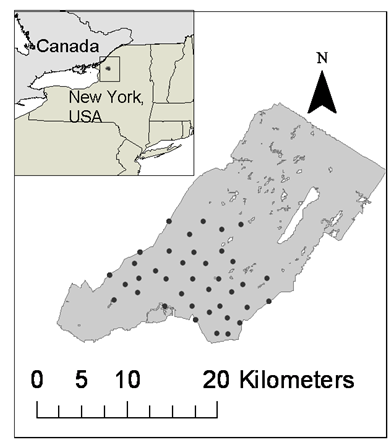
\includegraphics[height=3in,width=2.28in]{Ch3-Closed/figs/hairsnares.png}
\caption{Fort Drum Black bear study area and the 38 baited hair snare
  locations operated for 8 weeks during June and July, 2006.}
\label{closed.fig.fortdrum}
\end{figure}

{\small
\begin{verbatim}
library(scrbook)
data(beardata)
trapmat<-beardata$trapmat
nind<-dim(beardata$bearArray)[1]
K<-dim(beardata$bearArray)[3]
ntraps<-dim(beardata$bearArray)[2]

M=175
nz<-M-nind
Yaug <- array(0, dim=c(M,ntraps,K))

Yaug[1:nind,,]<-beardata$bearArray
y<- apply(Yaug,c(1,3),sum) # summarize by ind x rep
y[y>1]<- 1                 # toss out multiple encounters b/c
                           #    traditional CR models ignore space
\end{verbatim}
}


The raw data object, \mbox{\tt beardata\$bearArray} is a 3-dimensional
array $\mbox{\tt nind} \times \mbox{\tt ntraps} \times K$ of
individual encounter events (i.e., $y_{ijk} = 1$ if individual $i$ was
encountered in trap $j$ during occasion $k$, and 0 otherwise).  For
fitting model $M_{0}$ (or $M_{h}$, see below), it is sufficient to
reduce the data to individual encounter frequencies which we have
re-labeled \mbox{\tt y} above.  The {\bf BUGS} model file along with
commands to fit the model are as follows:

{\small
\begin{verbatim}
set.seed(2013)               # to obtain the same results each time
library(R2WinBUGS)
data0<-list(y=y,M=M,K=K)
params0<-list('psi','p','N')
zst=c(rep(1,nind),rbinom(M-nind, 1, .5))
inits =  function() {  list(z=zst, psi=runif(1), p=runif(1)) }

cat("
model {

psi~dunif(0, 1)
p~dunif(0,1)

for (i in 1:M){
   z[i]~dbern(psi)
   for(k in 1:K){
     tmp[i,k]<-p*z[i]
     y[i,k]~dbin(tmp[i,k],1)
      }
     }
N<-sum(z[1:M])
}
",file="modelM0.txt")

fit0 = bugs(data0, inits, params0, model.file="modelM0.txt",n.chains=3, 
       n.iter=2000, n.burnin=1000, n.thin=1,debug=TRUE,working.directory=getwd())
\end{verbatim}
}
This produces the following posterior
 summary statistics:
{\small
\begin{verbatim}
> print(fit0,digits=2)
Inference for Bugs model at "modelM0.txt", fit using WinBUGS,
 3 chains, each with 2000 iterations (first 1000 discarded)
 n.sims = 3000 iterations saved
           mean    sd   2.5%    25%    50%    75%  97.5% Rhat n.eff
psi        0.29  0.04   0.22   0.26   0.29   0.31   0.36    1  3000
p          0.30  0.03   0.25   0.28   0.30   0.32   0.35    1  3000
N         49.94  1.99  47.00  48.00  50.00  51.00  54.00    1  3000
deviance 489.05 11.28 471.00 480.45 488.80 495.40 513.70    1  3000

[... some output deleted ...]
\end{verbatim}
}
{\bf WinBUGS} did well in choosing an MCMC algorithm for this model --
we have $\hat{R} = 1$ for each parameter, and an effective sample size
of 3000, equal to the total number of posterior samples\footnote{This is even a little
suspicious....}.
We see that the posterior mean of $N$ under this
model is $49.94$ and a 95\% posterior interval is $(48,54)$.  We
revisit these data later in the context of more complex models.

In order to obtain an estimate of density, $D$, we need an area to
associate with the estimate of $N$, and in Chapt.  \ref{chapt.intro}
we already went through a number of commonly used procedures to
conjure up such an area, including buffering the trap array by the
home range radius, often estimated by the mean maximum distance moved
(MMDM) \citep{parmenter_etal:2003}, $1/2$ MMDM \citep{dice:1938} or
directly from telemetry data \citep{wallace_etal:2003}
\begin{comment}
I HAVE SEEN 2 PAPERS CITING OTIS ET AL 1978 IN THIS CONTEXT
BUT I ONLY FOUND THE SECITON WHERE THEY SUGGEST USING INFORMATION ON ANIMAL HOME RANGE AS
OBTAIN FROM TRAPPING DATA; I GUESS THIS DICE GUY SAID TO USE THE HOME RANGE RADIUS
AND PEOPLE JUST TRY TO GET AT THIS WHICHEVER WAY THEY CAN; BE IT RECAPTURES OR OTHER HOME RANGE INFORMATION XXXXX).
\end{comment}
Typically, the trap array is defined by the convex hull around the
trap locations, and this is what we applied a buffer to. We computed
the buffer by using an estimate of the mean female home range radius
(2.19 km) estimated from telemetry studies \citep{bales_etal:2005}
instead of using an estimate based on our relatively more sparse
recapture data.  For the Fort Drum study, the convex hull has an area
of $157.135$ km$^2$, and the buffered convex hull has an area of $277.011$
km$^2$.  To create this we used functions contained in the {\bf R}
package \mbox{\tt rgeos} and created a utility function \mbox{\tt
  bcharea} which is in our {\bf R} package \mbox{\tt scrbook}. The
commands are as follows:
\begin{verbatim}
library(rgeos)

bcharea<-function(buff,traplocs){
p1<-Polygon(rbind(traplocs,traplocs[1,]))
p2<-Polygons(list(p1=p1),ID=1)
p3<-SpatialPolygons(list(p2=p2))
p1ch<-gConvexHull(p3)
 bp1<-(gBuffer(p1ch, width=buff))
 plot(bp1, col='gray')
 plot(p1ch, border='black', lwd=2, add=TRUE)
 gArea(bp1)
}

bcharea(2.19,traplocs=trapmat)
\end{verbatim}
The resulting buffered convex hull is shown in Fig. \ref{closed.fig.bch}.
\begin{figure}[ht]
\begin{center}
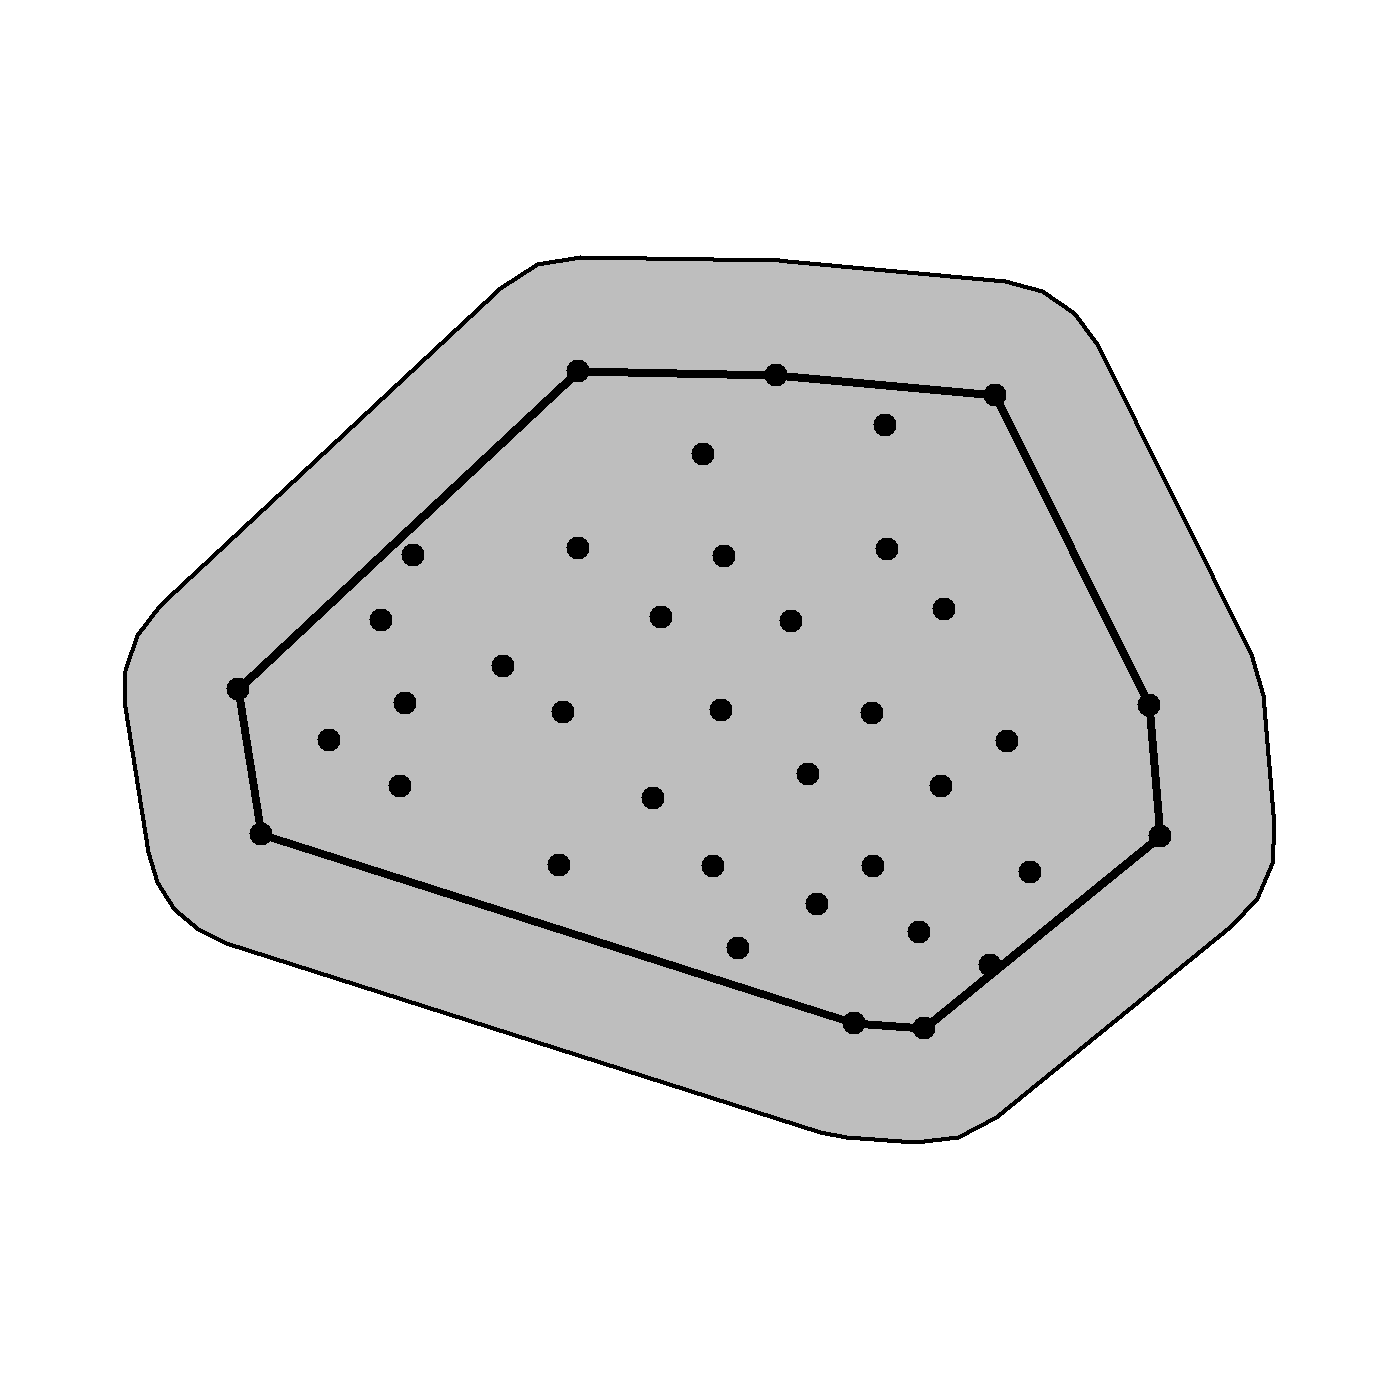
\includegraphics[height=3in,width=3in]{Ch3-Closed/figs/bufferedCH}
\end{center}
\caption{Convex hull of the bear hair snare array at Fort Drum, NY buffered by mean female
home range radius (2.19 km).}
\label{closed.fig.bch}
\end{figure}

To conjure up a
density estimate under model $M_0$, we compute the appropriate
posterior summary of the ratio of $N$ and the prescribed area ($277.011$ km$^2$):
{\small
\begin{verbatim}
> summary(fit0$sims.list$N/277.011)
   Min. 1st Qu.  Median    Mean 3rd Qu.    Max.
 0.1697  0.1733  0.1805  0.1803  0.1841  0.2130

> quantile(fit0$sims.list$N/277.011,c(0.025,0.975))
     2.5%     97.5%
0.1696684 0.1949381
\end{verbatim}
}
which yields a density estimate of about $0.18$ ind/km$^2$, and a $95\%$ Bayesian
confidence interval of $(0.170, 0.195)$.

Our estimate 
of density should be reliable  if we have faith in our
stated value of the ``sample area''. Clearly though this is largely
subjective, and not something we can formally evaluate (or estimate) from the data.
 More importantly, what exactly is
the meaning of this area -- in what quantitative sense is it the ``effective sample
area''? -- and, in this context, how do we gauge bias
and/or variance of ``estimators'' of it? These are questions that, to
the best of our knowledge, have not been addressed in any generality,
if at all\footnote{We note that \citet{karanth_nichols:1998} and
  possibly others have computed 
  the variance of an estimated buffer strip, but do not provide a
  quantitative definition of effective sample area.}. 

\begin{comment}
How certain are we of this area? Can
we quantify our uncertainty about this quantity?
 More important, what exactly is
the meaning of this area and, in this context, how do we gauge bias
and/or variance of ``estimators'' of it? (i.e., what is it
estimating?).\footnote{Mention the delta approximation from
KARANTH AND NICHOLS (1998)?}
There is no theory to guide us in trying to answer these important questions.
\end{comment}

\section{Temporally varying and behavioral effects}
\label{closed.sec.timebehavefx}

The purpose of this chapter is mainly to emphasize the central
importance of the binomial model in capture-recapture and so we have
considered models for individual encounter frequencies---the number of
times individuals are captured out of $K$ samples.  Sometimes we can't
aggregate the encounter data for each individual, such as when
encounter probability varies over time among samples.  Time-varying
responses that are relevant in many capture-recapture studies are
``effort'' such as amount of search time, number of observers, or trap
nights, or when encounter probability varies over time or as a
function of date or season due to species behavior
\citep{kery_etal:2010}.  A common situation in many animal studies is
that in which there exists a ``behavioral response'' to trapping (even
if the animal is not physically trapped).
%For example, individuals might exhibit
%``trap happiness'' in response to baited traps. Conversely, individuals might learn
%to avoid traps (trap shyness) if the capture experience produces some negative
%stimulus.

Behavioral response is an important concept in animal studies
because individuals might learn to come to baited traps or avoid traps
due to trauma related to being encountered.  There are a number of
ways to parameterize a behavioral response to encounter. The
distinction between persistent and ephemeral was made by
\citet{yang_chao:2005} who considered a general behavioral response
model of the form:
\[
\mbox{logit}(p_{ik}) = \alpha_{0} + \alpha_{1} y_{i,k-1} + \alpha_{2} x_{ik}
\]
where $x_{ik}$ is a covariate indicator variable of previous capture
(i.e., $x_{ik} = 1$ if captured in any previous period). Therefore,
encounter probability changes depending on whether an individual was
captured in the immediate previous period (a Markovian or ephemeral behavioral
response; \citep{yang_chao:2005}), described by the term
$\alpha_{1} y_{i,k-1}$ or in {\it any} previous period (persistent behavioral
response), described by the term  $\alpha_{2} x_{ik}$.
%The former probably models a behavioral response due to
%individuals moving around their territory relatively slowly over time
%and the latter probably accommodates trap happiness due to baiting or
%shyness due to trauma.
Because spatial capture-recapture models allow us to include
trap-specific covariates, we can describe a 3rd type of behavioral
response---a local behavioral response that is trap-specific
\citep{royle_etal:2011jwm}. In this local behavioral response, the
encounter probability is modified for an individual trap depending on
previous capture in that trap.
Models with temporal effects are easy to describe and analyze in the {\bf BUGS} language
and we provide a number of examples in
Chapt. \ref{chapt.covariates} and elsewhere.


\section{ Models with individual heterogeneity}
\label{closed.sec.modelmh}

Models in which encounter probability varies by individual, say
$p_{i}$, have a long history in capture-recapture and, indeed, this
so-called ``model $M_h$'' is one of the elemental capture-recapture
models in \citep{otis_etal:1978}. Conceptually, we imagine that 
the individual-specific encounter probability
parameters, $p_{i}$, are random variables distributed according to
some probability 
distribution, $[\theta]$. We denote this basic model assumption as
$p_{i} \sim [\theta]$. This type of model is similar in concept to
extending a GLM to a GLMM but in the capture-recapture context $N$ is
unknown.  The basic class of models is often referred to as ``model
$M_h$'' ('h' for heterogeneity), but really this is a broad class of models, each being
distinguished by the specific distribution assumed for $p_{i}$.  There
are many different varieties of model $M_{h}$ including parametric and
various 
non-parametric approaches
\citep{burnham_overton:1978, norris_pollock:1996, pledger:2000}. One
important practical matter is that estimates of $N$ can be extremely
sensitive to the choice of heterogeneity model
\citep{fienberg_etal:1999, dorazio_royle:2003, link:2003}. Indeed,
\citet{link:2003} showed that in some cases it's possible to find
models that yield precisely the same expected data, yet produce wildly
different estimates of $N$. In that sense, $N$ for most practical
purposes is not identifiable across classes of different heterogeneity
models, and
this should be understood before fitting any such model. One solution
to this problem is to seek to model explicit factors that contribute
to heterogeneity, e.g., using individual covariate models (See
\ref{closed.sec.indcov} below). Indeed, spatial capture-recapture
models seek to do just that, by modeling heterogeneity due to the
spatial organization of individuals in relation to traps or other
encounter mechanism.  For additional background and applications of
model $M_{h}$ see \citet[][Chapt. 6]{royle_dorazio:2008} and
\citet[][Chapt. 6]{kery_schaub:2011}.

Model $M_{h}$ has important historical relevance to spatial
capture-recapture situations \citep{karanth:1995} because
investigators recognized that the juxtaposition of individuals with
the array of trap locations should yield heterogeneity in encounter
probability, and thus it became common to use some version of model $M_h$
in spatial trapping arrays to estimate $N$.  While this doesn't
resolve the problem of not knowing the area relevant to $N$, it does
yield an estimator that accommodates the heterogeneity in $p$ induced
by the spatial aspect of capture-recapture studies.

To see how this juxtaposition induces heterogeneity, we have to
understand the relevance of movement in capture-recapture models.
Imagine a quadrat that can be uniformly searched by a crew of
biologists for some species of reptile (see
\citet{royle_young:2008}).  Figure \ref{closed.fig.quadrat} shows a
sample quadrat searched repeatedly over a period of time. Further,
suppose that the species exhibits some sense of spatial fidelity in the
form of a home range or territory, and individuals move about their
home range (home range centroids are given by the blue dots) in some
kind of random fashion.
%It is natural to think about it in terms of a
%movement process and sometimes that movement process can be modeled
%explicitly using hierarchical models \citep{royle_young:2008,
%  royle_etal:2011mee}.
Heuristically, we imagine that each individual in
the vicinity of the study area is liable to experience variable
exposure to encounter due to the overlap of its home range with the
sampled area - essentially the long-run proportion of times the
individual is within the sample plot boundaries, say $\phi$. We
might model the exposure of an individual to capture by supposing that
$z_{i} = 1$ if individual $i$ is available to be captured (i.e.,
within the survey plot) during any sample, and $0$ otherwise. Then,
$\Pr(z_{i}=1) = \phi$.  In the context of spatial studies, it is
natural that $\phi$ should depend on {\it where} an individual lives,
i.e., it should be individual-specific $\phi_{i}$
\citep{chandler_etal:2011}. This system describes, precisely, that of
``random temporary emigration'' \citep{kendall_etal:1997} where $\phi_{i}$
is the individual-specific probability of being ``available'' for
capture.

Conceptually, SCR models aim to deal with
this problem of variable exposure to sampling due to movement in the
proximity of the trapping array explicitly and formally with auxiliary
spatial information.  If individuals are detected with probability
$p_{0}$, {\it conditional} on $z_{i} = 1$, then the marginal
probability of detecting  individual $i$ is
\[
 p_{i} = p_{0}\phi_{i}
\]
so we see clearly that individual heterogeneity in encounter
probability is induced as a result of the juxtaposition of individuals
(i.e., their home ranges) with the sample apparatus and the movement
of individuals about their home range.

\begin{figure}
\begin{center}
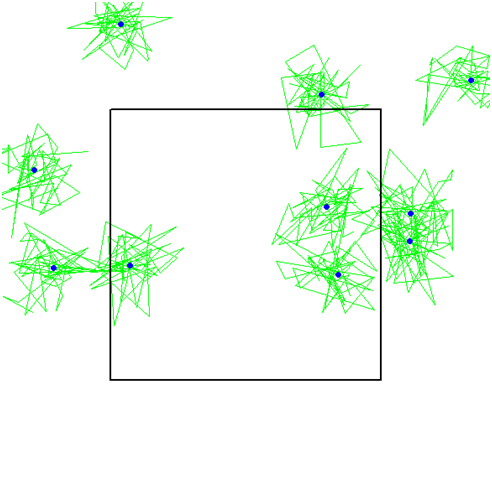
\includegraphics[height=3in]{Ch3-Closed/figs/quadrat}
\end{center}
\caption{A quadrat searched for lizards over some period of time
  (simulated data). The locations of encounter for each of 10 lizards are
  connected by lines---the dots are activity centers.}
\label{closed.fig.quadrat}
\end{figure}

We will work with a specific type of model $M_{h}$ here which is a
natural extension of
the basic binomial observation model of model $M_{0}$ so
that
\[
\mbox{logit}(p_{i}) = \mu + \eta_{i}
\]
where $\mu$ is a fixed parameter (the mean) to be estimated, and
$\eta_{i}$ is an individual random effect assumed to be normally distributed:
\[
\eta_{i} \sim \mbox{Normal}(0, \sigma_{p}^2)
\]
We could as well combine these two steps and write $\mbox{logit}(p_{i}) \sim \mbox{Normal}(\mu,\sigma_{p}^2)$.
This ``logit-normal mixture'' was analyzed by
\citet{coull_agresti:1999} and elsewhere. It is a natural extension of
the basic model with constant $p$, as a mixed GLMM, and similar models
occur throughout statistics. It is also natural to consider a beta
prior distribution for $p_{i}$ \citep{dorazio_royle:2003} and
so-called ``finite-mixture'' models are also popular
\citep{norris_pollock:1996, pledger:2000}. In the latter, individuals
are assumed to belong to a finite number of latent classes, each of
which has its own capture probability.


\subsection{Analysis of Model $M_h$}

If $N$ is known, it is worth taking note of the essential simplicity
of model $M_h$ as a binomial GLMM.  This is a type of model that is
widely applied throughout statistics using
standard methods of inference based either on integrated likelihood
\citep{laird_ware:1982, berger_etal:1999}, which we discuss in
Chapt. \ref{chapt.mle}, or standard Bayesian
methods. However, because $N$ is not known, inference is somewhat more
challenging. We address that here using Bayesian analysis based on
data augmentation. Although we use data augmentation in the context of
Bayesian methods here, we note that
heterogeneity models formulated under DA are easily analyzed by
conventional likelihood methods as zero-inflated binomial mixtures
\citep{royle:2006} and more traditional analysis of model $M_h$ based on
integrated likelihood, without using data augmentation, has been
considered by \citet{coull_agresti:1999}, \citet{dorazio_royle:2003},
and others.

As with model $M_{0}$, we have the Bernoulli model for the
zero-inflation variables: $z_{i} \sim \mbox{Bern}(\psi)$ and the model
of the observations expressed conditional on these latent variables
$z_{i}$. For $z_{i}=1$, we have a binomial model with
individual-specific $p_{i}$:
\[
y_{i}|{z_{i} \! = \! 1} \sim \mbox{Binomial}(K,p_{i})
\]
and otherwise $y_{i} |{ z_{i} \! = \! 0} \sim 1(y=0)$. Further, we
prescribe a distribution for $p_{i}$. Here we assume
\[
\mathrm{logit}(p_{i}) \sim \mbox{Normal}(\mu,\sigma^2)
\]
For prior distributions we assume
$p_{0} = \mbox{logit}^{-1}(\mu) \sim
\mbox{Uniform}(0,1)$ and, for the variance component
$\sigma \sim \mbox{Uniform}(0,B)$ for some large $B$.
\begin{comment}
The basic {\bf BUGS} description for this model is given as follows:
{\small
\begin{verbatim}
model{

p0 ~ dunif(0,1)       # prior distributions
mup<- log(p0/(1-p0))
sigmap ~ dunif(0,10)
taup<- 1/(sigmap*sigmap)
psi~dunif(0,1)

for(i in 1:(nind+nz)){
  z[i]~dbern(psi)     # zero inflation variables
  lp[i] ~ dnorm(mup,taup) # individual effect
  logit(p[i])<-lp[i]
  mu[i]<-z[i]*p[i]
  y[i]~dbin(mu[i],K)  #  observation model
 }

N<-sum(z[1:(nind+nz)])  # N is a derived parameter
}
\end{verbatim}
}
\end{comment}
Another common default prior is to assume
$\tau = 1/\sigma^{2} \sim \mbox{Gamma}(.1,.1)$, although we usually
choose the $\sigma \sim \mbox{Uniform}(0,B)$.



\subsection{Analysis of the Fort Drum data with model $M_{h}$}
\label{closed.sec.Mhbear}

Here we provide an analysis of the Fort Drum bear survey data using
the  
 logit-normal heterogeneity model, and we 
used data augmentation to produce a data
set of $M=700$ individuals.  
%We note that 
%the model runs effectively in {\bf WinBUGS} but sometimes with apparently
%inefficient mixing for reasons that may be related to bad starting
%values. In some cases this was resolved if we supplied starting values
%for the $\mbox{logit}(p_{i})$ parameters and $\tau$. 
We have so far mostly used 
{\bf
  WinBUGS} but for most of our operational analyses now we are
transitioning to the use of {\bf JAGS} run from within {\bf R} using the useful packages 
 \mbox{\tt R2jags} or \mbox{\tt rjags}.  The function \mbox{\tt jags}
 from the \mbox{\tt R2jags} package runs essentially like the
 \mbox{\tt bugs} function
which we demonstrate 
as follows for setting
 up and running model $M_{h}$ for the Fort Drum bear data:
{\small
\begin{verbatim}
[... get data as before ....]

set.seed(2013)

cat("
model{
p0 ~ dunif(0,1)       # prior distributions
mup<- log(p0/(1-p0))
sigmap ~ dunif(0,10)
taup<- 1/(sigmap*sigmap)
psi~dunif(0,1)

for(i in 1:(nind+nz)){
  z[i]~dbern(psi)     # zero inflation variables
  lp[i] ~ dnorm(mup,taup) # individual effect
  logit(p[i])<-lp[i]
  mu[i]<-z[i]*p[i]
  y[i]~dbin(mu[i],K)  #  observation model
 }

N<-sum(z[1:(nind+nz)])
}
",file="modelMh.txt")

data1<-list(y=y, nz=nz, nind=nind,K=K)
params1= c('p0','sigmap','psi','N')
inits =  function() {list(z=as.numeric(y>=1), psi=.6, p0=runif(1),
          sigmap=runif(1,.7,1.2),lp=rnorm(M,-2)) }
library(R2jags)
wbout = jags(data1, inits, params1, model.file = "modelMh.txt", n.chains = 3, 
            n.iter = 1010000, n.burnin =10000, working.directory = getwd())
\end{verbatim}
}

We provide an {\bf R} function \mbox{\tt modelMhBUGS} in the package
\mbox{\tt scrbook} which will fit the model using either {\bf JAGS} or
{\bf WinBUGS} as specified by the user.  In addition, for fun, we
construct our own MCMC algorithm using a Metropolis-within-Gibbs
algorithm for model $M_{h}$ in Chapt. \ref{chapt.mcmc}, where we also
develop MCMC algorithms for spatial capture-recapture models.  Using
the {\bf WinBUGS} option in \mbox{\tt modelMhBUGS}, we ran 3 chains of 1
{\it million} iterations (mixing is poor for this model and this data
set), which produced the posterior distribution for $N$ shown in
Fig. \ref{closed.fig.bearMh}. Posterior summaries of parameters are
given as follows\footnote{The reported \mbox{\tt n.sims} printed appears
  to be an error in the \mbox{\tt R2WinBUGS} package}: 
{\small
\begin{verbatim}
> print(wbout,digits=3)
Inference for Bugs model at "modelMh.txt", fit using WinBUGS,
 3 chains, each with 1010000 iterations (first 10000 discarded)
 n.sims = 2970000 iterations saved
            mean     sd    2.5%     25%     50%     75%   97.5%  Rhat n.eff
p0         0.072  0.056   0.002   0.027   0.060   0.106   0.203 1.008   540
sigmap     2.096  0.557   1.215   1.694   2.025   2.424   3.373 1.003   820
psi        0.176  0.101   0.084   0.117   0.147   0.198   0.458 1.006   650
N        122.695 69.897  62.000  82.000 102.000 137.000 319.000 1.006   630
deviance 187.089 17.998 155.400 174.400 185.900 198.500 225.700 1.002  3600

[... output deleted ... ]
\end{verbatim}
}


We used $M=700$ for this analysis and we
note that  while the posterior mass of $N$ is concentrated away from this
upper bound (Fig. \ref{closed.fig.bearMh}), the posterior has an
extremely long right tail, with some MCMC draws at the upper
boundary $N=700$, suggesting that an even higher value of $M$ may be
called for. 
%To make this plot and summarize the posterior distribution
%of model parameters, we have to grab the output from running {\bf
%  JAGS} in a slightly different manner -- the returned object is a
%list which contains {\bf R2WinBUGS}-like output in the list \mbox{\tt
%  BUGSoutput}. XXXX OBSOLETE? XXXXX
To characterize the posterior distribution of density we produce the
relevant summaries of the posterior distribution of $D  = N/277.11$
(recall 
the buffered area of the convex hull is 277.11 $km^2$):
{\small
\begin{verbatim}
> summary(wbout$sims.list$N/277.11)
   Min. 1st Qu.  Median    Mean 3rd Qu.    Max. 
 0.1696  0.2959  0.3681  0.4428  0.4944  2.5260 

> quantile(wbout$sims.list$N/277.11,c(0.025,0.50,0.975))
     2.5%       50%     97.5% 
0.2237379 0.3680849 1.1511674 
\end{verbatim}
}
so the point estimate, characterized by the posterior median, is around
$0.37$ bears per square km and a 95\% Bayesian credible interval is
$(0.224, 1.151)$.


\begin{figure}[ht]
\centering
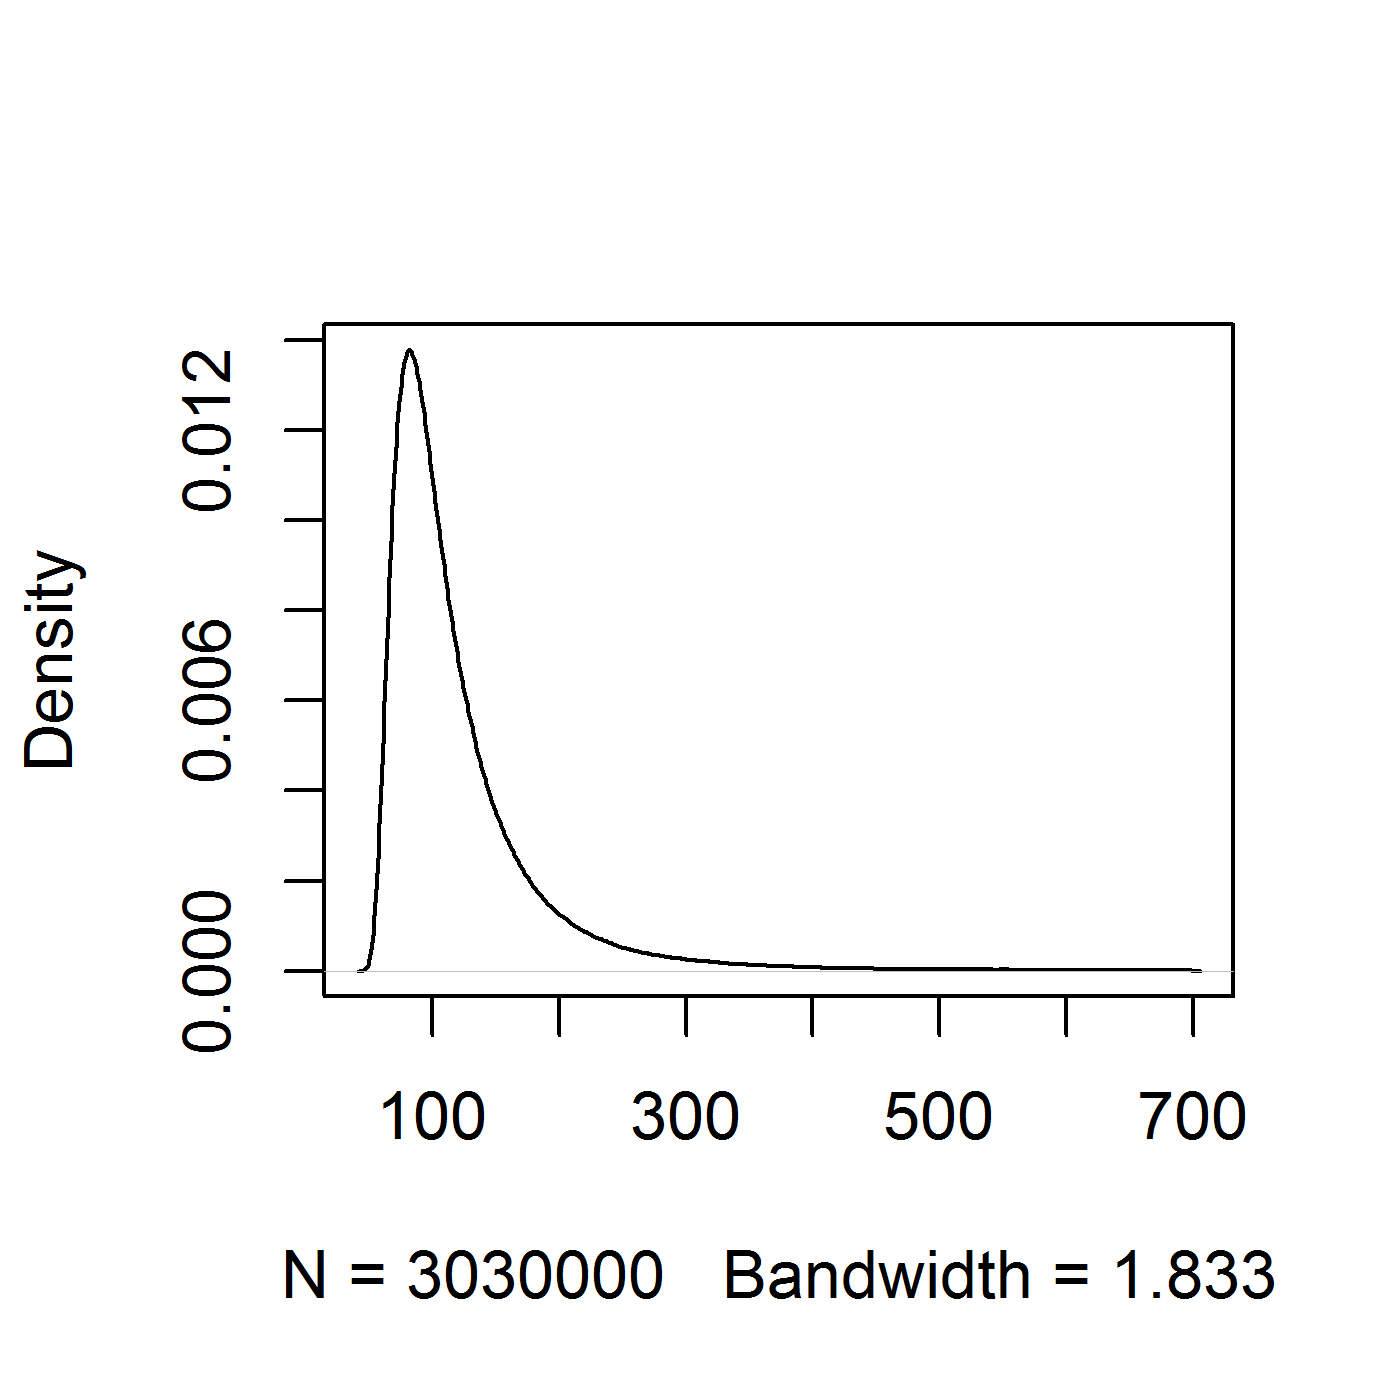
\includegraphics[height=3.5in,width=3.5in]{Ch3-Closed/figs/bear-modelMh-post-v2}
\caption{Posterior of $N$ for Fort Drum bear study data under the
logit-normal version of model $M_h$.
}
\label{closed.fig.bearMh}
\end{figure}

\subsection{Comparison with MLE}

The posterior of $N$ is highly skewed; therefore, we see that the 
posterior mean
($N=122.7$) is considerably higher than the posterior median
($N=102$).
Further, it may be surprising that these posterior
summaries do not compare well with the MLE.
We used 
the {\bf R} code contained in Panel 6.1 from
\citet{royle_dorazio:2008} to obtain the 
MLE of $\log(n_{0})$, the logarithm of the number of uncaptured
individuals, is $\widehat{\log(n0)} = 3.86$ and therefore $\hat{N} =
\exp(3.86)+47 = 94.47$, much higher than the mode 
shown in Fig. \ref{closed.fig.bearMh}.
To see this, we compute the posterior mode\index{posterior mode,
  calculation of} by finding
the posterior value of $N$ with the highest mass.
 Because $N$ is discrete, we can  use
the \mbox{\tt table()} function in {\bf R} and find the most frequent value
\footnote{For a continuous random variable we can use the function
 \mbox{\tt
    density()} to smooth the posterior samples and obtain the mode.}.
% Here are the
%commands for doing this:
%\begin{verbatim}
% N<-table(jout$BUGSoutput$sims.list$N)
% N[N==max(N)]
%   84 
% 41961 
%\end{verbatim}
If we want to smooth out some of the Monte
Carlo error a bit, we can use a smoother of some sort applied to the tabled
posterior frequencies of $N$. Here we use a smoothing spline ({\bf R}
function \mbox{\tt smooth.spline}) with the
degree of smoothing chosen by cross-validation:
{\small
\begin{verbatim}
> N<-table(jout$BUGSoutput$sims.list$N)
> xg<-as.numeric(names(N))

> sp<- smooth.spline(xg,N,cv=TRUE)
 
> sp  

Call:
smooth.spline(x = xg, y = N, cv = TRUE)

Smoothing Parameter  spar= 0.09339815  lambda= 8.201724e-09 (17 iterations) 
Equivalent Degrees of Freedom (Df): 121.1825 
Penalized Criterion: 2544481 
PRESS: 5903.4 
\end{verbatim}
}
We obtain the mode of the smoothed frequencies as follows:
\begin{verbatim}
sp$x[sp$y==max(sp$y)]
[1] 82
\end{verbatim}
%The \mbox{\tt df} argument controls the degree of smoothing and we can
%play around with that value or choose it using some method such as cross-validation
%find in this case that the modal value (i.e., 82) is not too sensitive
%to the smoothing parameter but this should be checked in any specific
%instance\footnote{we need to give examples of using \mbox{\tt
%    density()} to obtain modes}.


\begin{comment}
We note that any scalar summary of the posterior distribution is
pretty inconsistent with the MLE. 
We used 
the {\bf R} code contained in Panel 6.1 from
\citet{royle_dorazio:2008} to obtain the 
MLE of $\log(n_{0})$, the logarithm of the number of uncaptured
individuals, is $\widehat{\log(n0)} = 3.86$ and therefore $\hat{N} =
\exp(3.86)+47 = 94.47$ which is considerably higher than the mode
shown in Fig. \ref{closed.fig.bearMh}.
%\footnote{We note that the result is inconsistent with Gardner et
%  al. (2009) who reported an MLE of 104.1 ($density = 0.437
%  inds/km^2$) although we do not know the reason for this at the
%  present time.}
%To convert this to density we use the buffered area
%as computed above (255.3 $km^2$)\footnote{WRONG \#} and perform the
%required summary analysis on the posterior samples of $N$, which
%results in about $0.37$ individuals/$km^2$. The reader should carry
%out this analysis to confirm the estimates, and also obtain the $95\%$
%confidence interval.
\end{comment}


We don't dwell too much on the difference, but we do note here that
the posterior distribution for the parameters of this model, for the
Fort Drum data set, are very sensitive to the prior
distributions. While MLEs are invariant to transformation of the
parameters, the posterior distribution definitely is {\it not}
invariant. In the present case, the use of a $\mbox{Uniform}(0,1)$
prior for $p_{0} = \mbox{logit}^{-1}(\mu)$ is somewhat
informative---in particular, it is not at all ``flat'' on the scale of
$\mu$, and this affects the posterior.  We generally always recommend
use of a $\mbox{Uniform}(0,1)$ prior for $\mbox{logit}^{-1}(\mu)$ in
such models. That said, we were surprised at this result, and we
experimented with other prior configurations including putting a flat
prior on $\mu$ directly. That specific prior suggests the possibility
that the posterior distribution may be improper for that prior
specification. This kind of small sample instability has been widely
noted in model $M_h$ \citep{fienberg_etal:1999, dorazio_royle:2003},
as has extreme sensitivity to the specific form of model $M_{h}$
\citep{link:2003}.  In summary, while the mode is well-defined, the
data set is relatively sparse and hence inferences are poor and
sensitive to model choice.






\begin{comment}

\subsection{Exercises related to model $M_h$}

\begin{itemize}
\item[(1)] Enclose the MCMC algorithm in an R function and provide
  arguments for some of the parameters of the function that a user
  might wish to modify.
\item[(2)] Execute the function and compare the results to those
  generated from WinBUGS in the previous section
\item[(3)] Note that the prior distribution for the ``mean'' parameter
  is given on $p_0=\exp(\mu)/(1+exp(\mu))$.  Reformulate the algorithm
  with a flat prior on $\mu$ and see what happens. Contemplate this.
\item[(4)] Using Bayes rule, figure out the full conditional for
  $z_{i}$ so that you don't have to use MH for that one. It might be
  more efficient. Is it?
\item[(5)] Modify the MCMC algorithm so that the prior for $\mu_{p}$
  is an improper flat prior. i.e., $[\mu_{p}] \propto 1$. Describe the
  posterior distribution of $N$.
\end{itemize}

\end{comment}



\section{Individual Covariate Models: Toward Spatial Capture-Recapture}
\label{closed.sec.indcov}


A standard situation in capture-recapture models is when a covariate
which is thought to influence encounter probability is measured for
each individual.  As with other closed population models, we begin
with the basic binomial observation model:
\[
y_{i} \sim \mbox{Binomial}(K, p_{i})
\]
and we assume also  a model for encounter probability according to:
\begin{equation}
 \mbox{logit}(p_{i}) = \alpha_0 + \alpha_1 x_{i}
\label{closed.eq.ha}
\end{equation}
where $x_i$ is the covariate value for individuals $i$ and the
parameters $\bm{\alpha}$ are the regression coefficients. Classical
examples of covariates influencing detection probability are type of
animal (juvenile/adult or male/female), a continuous covariate such as
body mass \citep[][ch. 6]{royle_dorazio:2008}, or a discrete covariate
such as group or cluster size. For example, in models of aerial survey
data, it is natural to model the detection probability of a group as a
function of the observation-level individual covariate, ``group size''
\citep{royle:2008, royle:2009, langtimm_etal:2011}.

Such ``individual covariate models'' are similar in structure to model
$M_{h}$, except that the individual effects are {\it observed} for the
$n$ individuals that appear in the sample. These models are important
here because spatial capture-recapture models can be described
precisely as a form of individual covariate model, where the covariate
describes {\it where} the individual is located in relation to the
trapping array.  Specifically, they are such models, but where the
individual covariate is a partially observed latent variable for
captured individuals.  Unlike model $M_h$, in individual covariate
models (and SCR models) we do have some direct information about the
latent variable, which comes from the spatial locations/distribution
of individual recaptures.

Traditionally, estimation of $N$ in individual covariate models is
achieved using methods based on ideas of unequal probability sampling
(i.e., Horvitz-Thompson estimation\footnote{For a  quick summary of
  the idea see: \\
  \url{http://en.wikipedia.org/wiki/Horvitz-Thompson_estimator}};
\citet{huggins:1989},
\citet{alho:1990} and \citet{borchers_etal:2002}). An estimator of $N$ is
\[
\hat{N} = \sum_{i=1}^{n} \frac{1}{\tilde{p}_{i}}
\]
where $\tilde{p}_{i}$ is the probability that individual $i$ appeared
in the sample.  That is, $\tilde{p}_{i} = \Pr(y_{i}>0)$
where, in closed population capture-recapture models,
\[
\Pr(y_{i}>0) = 1- (1-p_{i})^K
\]
where $p_{i}$ is a function of parameters $\alpha_{0}$ and $\alpha_{1}$
according to Eq. \ref{closed.eq.ha}.  In practice, parameters are
estimated from the conditional-likelihood of the observed encounter
histories which is, for observation $y_{i}$,
\begin{equation}
{\cal L}_{c}( {\bm \alpha} | y_{i}) = \frac{ \mbox{Binomial}(y_{i}|{\bm \alpha}) } { \tilde{p}_{i}}.
\label{closed.eq.cond}
\end{equation}
This derives from a straightforward application of the law of total
probability. Conceptually, we partition $\Pr(y)$ according to 
$\Pr(y) = \Pr(y|y>0)\Pr(y>0) + \Pr(y|y=0)\Pr(y=0)$. For any positive
value of $y$ the 2nd term is necessarily 0, and so we rearrange to
obtain
$\Pr(y|y>0) = \Pr(y)/\Pr(y>0)$ which, in the specific case where
$\Pr(y)$ is the 
binomial pmf produces Eq. \ref{closed.eq.cond}.


Here we take a formal model-based approach to Bayesian analysis of
such models based on the joint likelihood using data augmentation
\citep{royle:2009}. Classical likelihood analysis of the so-called
``full likelihood'' is covered by \citet{borchers_etal:2002}.  For
Bayesian analysis of individual covariate models, because the
individual covariate is unobserved for the $n_{0} = N-n$ uncaptured
individuals, we require a model to describe variation among
individuals, essentially allowing the sample to be extrapolated to the
population.  For example, if we have a continuous trait measured on
each individual, then we might assume that $x$ has a normal distribution:
\[
x_{i} \sim \mbox{Normal}(\mu,\sigma^{2})
\]
Data augmentation can be applied directly to this class of models. In
particular, reformulation of the model under DA yields a basic
zero-inflated binomial model of the form:
\begin{eqnarray*}
z_{i} &\sim& \mbox{Bernoulli}(\psi) \; \; \; i=1,2,\ldots,M\\
y_{i}|{z_{i}\! =\! 1} &\sim& \mbox{Binomial}(K,p_{i}(x_{i})) \\
y_{i} |{ z_{i}\! =\! 0} &\sim& 1(y=0)  \\
x_{i} & \sim & \mbox{Normal}(\mu,\sigma^{2})
\end{eqnarray*}
Fully spatial capture-recapture models use this formulation with a
latent covariate that is directly related to the individual detection
probability (see next section). As with the previous models,
implementation is trivial in the {\bf BUGS} language. The {\bf BUGS}
specification is very similar to that for model $M_h$, but we require
the distribution of the covariate to be specified, along with priors
for the parameters of that distribution.


\subsection{Example: Location of capture as a covariate.}

Here we consider a special type of individual covariate model that is
especially relevant to spatial capture-recapture.  Intuitively, some
measure of distance from home range center to traps for an individual
should be a reasonable covariate to explain heterogeneity in encounter
probability, i.e., individuals with more exposure to traps should have
higher encounter probabilities and vice versa. So we can imagine {\it
  estimating} such a quantity, say average distance from home range
center to ``the trap array'', and then using it as an individual
covariate in capture-recapture models.  A version of this idea was put
forth by \citet{boulanger_mclellan:2001} (see also \citet{ivan:2012}),
but using the Huggins-Alho estimator and with covariate ``distance
from home range center to edge'' of the trapping array, where the home
range center is estimated by the average capture location.  This is
intuitively appealing because we can imagine, in some kind of an ideal
situation where we have a dense grid of traps over some geographic
region, that the average location of capture would be a decent
estimate (heuristically) of an individual's home range center.  We
provide an example of this type of heuristically motivated approach
using a fully model-based individual covariate model described above
analyzed by data augmentation. We take a slightly different approach
than that adopted by \citet{boulanger_mclellan:2001}. By analyzing the
full likelihood and placing a prior distribution on the individual
covariate, we will resolve the problem of having an ill-defined
sampled area.  After you read later chapters of this book, it will be
apparent that SCR models represent a formalization of this heuristic
procedure.


% A practical limitation of using sample estimates of individual covariates such
% as this is that it induces other statistical problems. Namely, 
%it does not readily accommodate the
%inherent and heterogeneous variation of the  measured covariate, nor
%does it  provide a solution to the problem that the trap area
%is not well-defined.



For our purposes here, we define the individual covariate $x_{i} = ||{\bf s}_{i} - {\bf
  x}_{0}||$ where ${\bf s}_{i}$ is the average encounter location of
individual $i$ and ${\bf x}_{0}$ is the centroid of the trap array.
In practice, people have
used distance from edge of the trap array but that is less easy to
quantify, as ``edge'' itself is not precisely defined.
Conceptually, individuals in the middle of the array should have a
higher probability of encounter and, as $x_{i}$ increases, $p_{i}$
should therefore decrease. We note that we have defined ${\bf s}_{i}$
in terms of a sample quantity---the observed mean---which is ad hoc
but consistent with the use of individual covariate models
 in the literature.  For an
expansive, dense trapping grid we might expect the sample mean
encounter location to be a good estimate of home range center but,
clearly this is biased for individuals that live around the edge (or
off) the trapping array. 
 A key point is that
${\bf s}_{i}$ is missing for each individual that is not encountered
and so  $x_{i}$ is also missing. Therefore, it is a latent variable, or random
effect, and we need  to specify a probability distribution
for it.  As a measurement of distance we know it must be
positive-valued, and it seems sensible that an individual located
extremely far from the array of traps would not be captured.
Therefore, let's assume that $x_{i}$ is uniformly distributed from $0$ to some large number,
say $B$, beyond which it would be difficult to imagine an
individual being captured by the trap array. For example, $B$ should be at a home
range diameter past the furthest trap from the center.  As such, we
use this distribution for the individual covariate ``distance from
center of the trap array''
\[
 x_{i} \sim \mbox{Uniform}(0,B)
\]
where $B$ is a specified constant, which we may choose to be
arbitrarily large.  


\subsection{Fort Drum Bear Study}


We have to do a little bit of data processing to fit this individual
covariate model to the Fort Drum data.  We need to compute the
individual covariate ${\bf x}_{i}$ (distance from the centroid of the
trapping array) using the {\bf R} function \mbox{\tt spiderplot}
provided in \mbox{\tt scrbook}. This function also produces the keen
plot shown in Fig. \ref{closed.fig.spiderplot} which we call a
``spider plot''.  The {\bf R} commands for obtaining the individual
covariate ``distance from trap centroid'' and making the spider plot
are as follows: 
\begin{verbatim}
library(scrbook)
data(beardata)
toad<- spiderplot(beardata$bearArray,beardata$trapmat)
xcent<-toad$xcent
\end{verbatim}

\begin{figure}
\centering
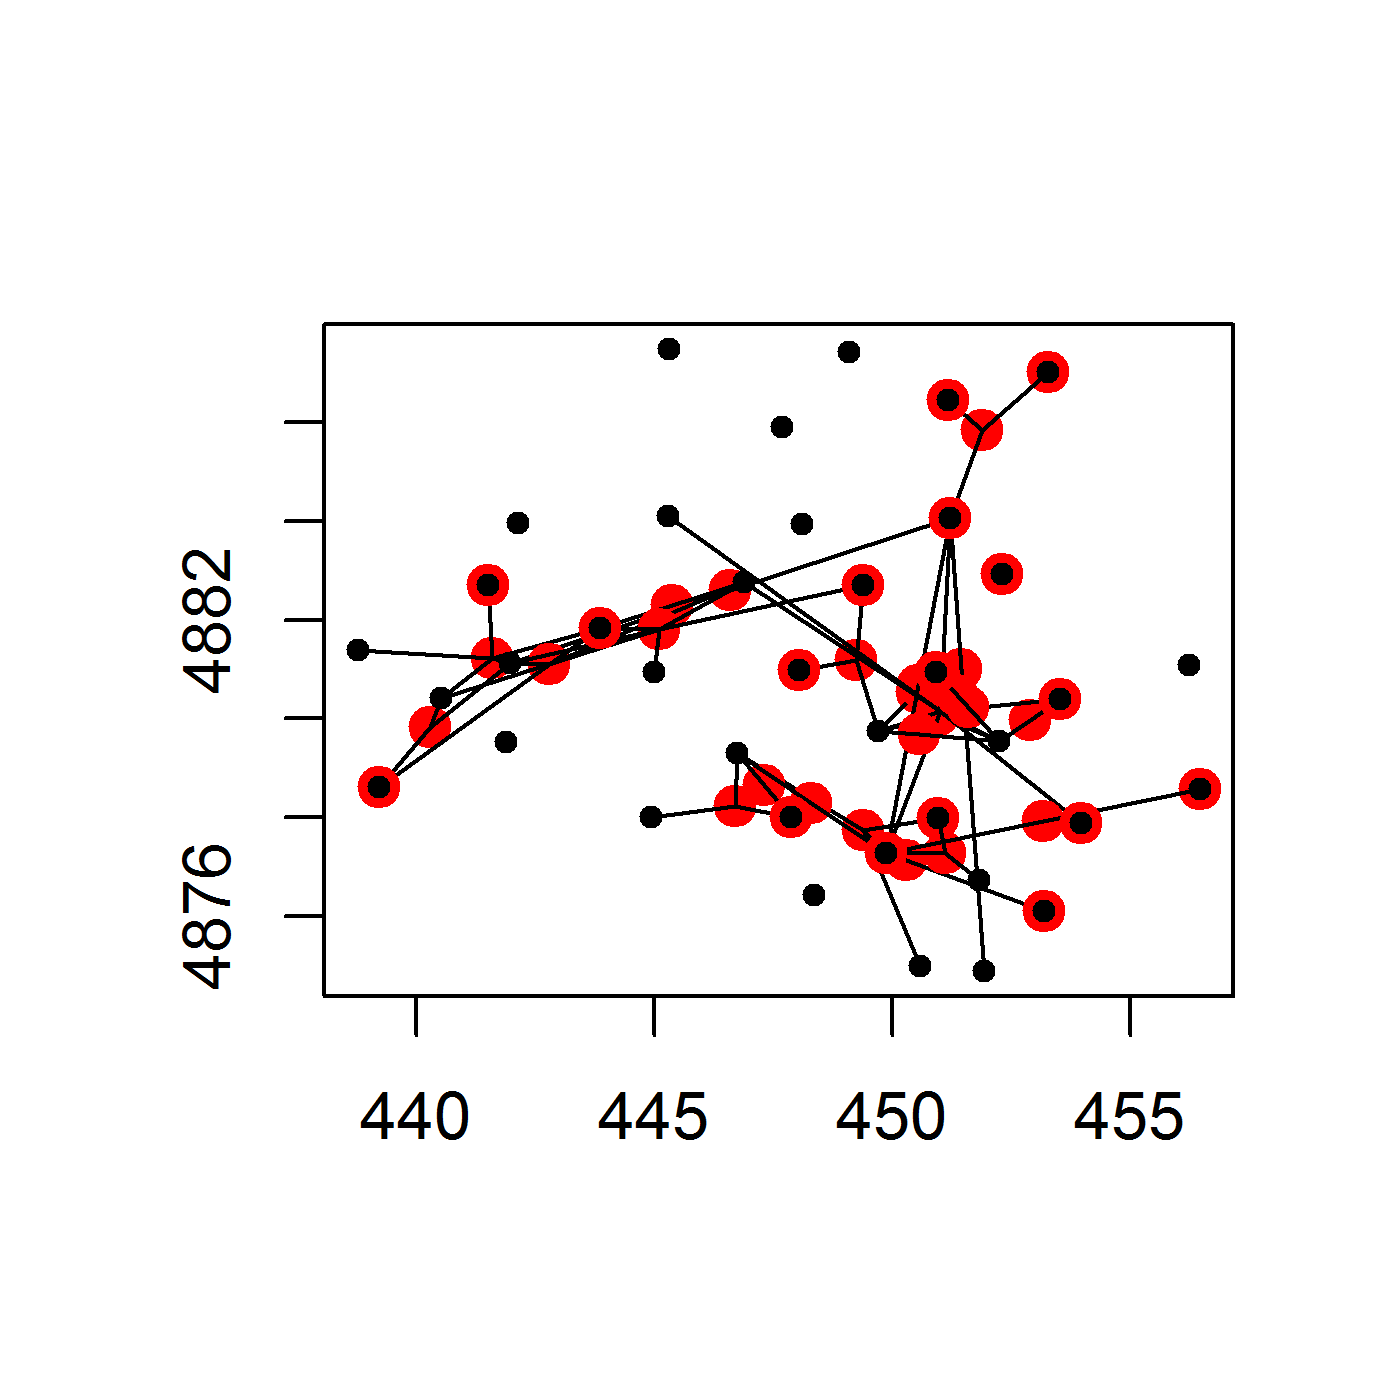
\includegraphics[height=3.5in,width=3.5in]{Ch3-Closed/figs/bear_spiderplot.png}
\caption{Spider plot of the Fort Drum study data.
The black dots represent the 47 trap locations with larger red dots
being the average capture location of each bear. i.e., its estimated home
range center. All traps in which a bear was captured are connected to
its estimated home range center with a line.
{\bf XXX note to Andy: change one of the dots to an X or something
  XXXXX }
}
\label{closed.fig.spiderplot}
\end{figure}

For the analysis of these data using the individual covariate
``distance from centroid'' we used $x_{i} \sim \mbox{Uniform}(0,B)$
with $B = 11.5$ $km^2$, which is about the distance from the array
center to the furthest trap.  Once we choose a value for $B$, the direct
implication is that the population size parameter, $N$, applies to the area
within 11.5 units of the trap centroid. We will see shortly that $N$
does, in fact, scale with our choice of $B$ to reflect the changing
area over which the $N$ individuals of the model reside.  The {\bf
  BUGS} model specification and {\bf R} commands to package the data
and fit the model are as follows: 
{\small
\begin{verbatim}
cat("
model{
p0 ~ dunif(0,1)       # prior distributions
alpha0<- log(p0/(1-p0))
psi~dunif(0,1)
beta~dnorm(0,.01)

for(i in 1:(nind+nz)){
  xcent[i]~dunif(0,B)
  z[i]~dbern(psi)     # DA variables
  lp[i] <- alpha0 + beta*xcent[i] # individual effect
  logit(p[i])<-lp[i]
  mu[i]<-z[i]*p[i]
  y[i]~dbin(mu[i],K)  #  observation model
 }
N<-sum(z[1:(nind+nz)])
}
",file="modelMcov.txt")

data2<-list(y=y,nz=nz,nind=nind,K=K,xcent=xcent,B=11.5)
params2<-list('p0','psi','N','beta')
inits =  function() {list(z=zst, psi=psi, p0=runif(1),beta=rnorm(1) ) }
fit2 =   bugs(data2, inits, params2, model.file="modelMcov.txt",
         n.chains=3, n.iter=11000, n.burnin=1000, n.thin=1)
\end{verbatim}
}
This produces the following posterior summary statistics:
{\small
\begin{verbatim}
Inference for Bugs model at "modelMcov.txt", fit using WinBUGS,
 3 chains, each with 11000 iterations (first 1000 discarded)
 n.sims = 30000 iterations saved
           mean    sd   2.5%    25%    50%    75%  97.5% Rhat n.eff
p0         0.54  0.07   0.40   0.50   0.54   0.59   0.67    1  1100
psi        0.34  0.05   0.25   0.31   0.34   0.37   0.44    1  3500
N         58.92  5.49  50.00  55.00  58.00  62.00  71.00    1  1900
beta      -0.25  0.06  -0.36  -0.29  -0.25  -0.21  -0.12    1   780
deviance 459.51 13.21 435.80 450.20 458.80 467.90 487.40    1  2600
\end{verbatim}
}

We note that the estimated $N$ is much lower than obtained by model
$M_h$ but there is a good explanation for this, discussed
subsequently. That issue notwithstanding, it is worth pondering how
this model could be an improvement (conceptually or technically) over
some other model/estimator including $M_0$ and $M_h$ considered
previously. Well, for one, we have accounted formally for
heterogeneity due to spatial location of individuals relative to
exposure to the trap array, characterized by the centroid of the
array. Moreover, we have done so using a model that is based on an
explicit mechanism, as opposed to a phenomenological one such as Model
$M_h$. Moreover, importantly, using our new model, {\it the estimated
  N applies to an explicit area which is defined by our prescribed
  value of $B$}. That is, this area is a fixed component of the model
and the parameter $N$ therefore has explicit spatial context, as the
number of individuals with home range centers less than $B$ from the
centroid of the trap array. As such, the implied ``effective area'' of
the trap array for a given $B$ is a precisely defined quantity---it is
that of a circle with with radius $B$.


\subsection{Extension of the Model}

The model developed in the previous section is not a very good model
for one important reason: Imposing a uniform prior distribution on $x$
implies that density is {\it not constant} over space. In particular,
this model implies that density {\it decreases} as we move away from the
centroid of the trap array.  That is, $x_{i} \sim \mbox{Uniform}(0,B)$
implies constant $N$ in each distance band from the centroid but
obviously the {\it area} of each distance band is increasing.  This is
one reason we have a lower estimate of density than that obtained
previously from model $M_h$ (Sec. \ref{closed.sec.Mhbear}) and also
why, if we were to increase $B$, we would see density continue to
decrease.

Fortunately, we are not 
restricted to use of this specific distribution for the individual
covariate. Clearly, it is a bad choice and, therefore, we should think
about whether we can choose a better distribution for $B$---one that
doesn't imply a decreasing density as distance from the centroid
increases.  Conceptually, what we want to do is impose a prior on
distance from the centroid, $x$, such that density is proportional to
the amount of area in each successive distance band as you move
farther away from the centroid.  In fact, theory exists which tells us
what the correct distribution of $x$ is: $2x/B^2$. This can be derived
by noting that $F(x) = \Pr(X<x) = (\pi x^2)/(\pi*B^{2})$ . Then, $f(x)
= dF/dx = 2*x/(B^{2})$. This is a sort of triangular distribution in
density induced because the incremental area in each additional
distance band increases linearly with radius (i.e., distance from
centroid). This can be verified empirically as follows:
{\small
\begin{verbatim}
 u<-runif(10000,-1,1)
 v<-runif(10000,-1,1)
 d<- sqrt(u*u+v*v)
 hist(d[d<1])
 hist(d[d<1],100)
 hist(d[d<1],100,probability=TRUE)
 abline(0,2)
\end{verbatim}
}

It would be useful if we could describe this distribution directly in {\bf
  BUGS} but there is not a built-in way to do so. However, we can 
implement a discrete version of the pdf\footnote{We might
also be able to use what is referred to in {\bf WinBUGS} jargon as the
``zeros trick'' (see {\it Advanced BUGS tricks} in the manual)
although we haven't pursued this approach.}. To do this, 
we break $B$ into $L$
distance classes of width $\delta$, with probabilities proportional to
$2*x$. In particular, if we denote the cut-points by $g_{1}=0,g_{2},
\ldots, g_{L+1}=B$ and the interval midpoints are $m_{i} =
g_{i+1}-\delta$.  
Then the interval probabilities are, approximately, $p_{i} =
2 m_{i} \delta/(B^{2})$, which we can compute once and then
pass them to {\bf BUGS} as data.
The {\bf R} commands for doing all of this (noting that we have
already loaded and processed the Fort Drum bear data) are given in the
following {\bf BUGS} code:
{\small
\begin{verbatim}
delta<-.2
xbin<-xcent%/%delta  + 1
Dgrid<- seq(delta,Dmax,delta)
xprobs<- delta*(2*Dgrid/(Dmax*Dmax))
xprobs<-xprobs/sum(xprobs)

cat("
model{
p0 ~ dunif(0,1)       # prior distributions
alpha0<- log(p0/(1-p0))
psi~dunif(0,1)
beta~dnorm(0,.01)

for(i in 1:(nind+nz)){
  xbin[i]~dcat(xprobs[])
  z[i]~dbern(psi)                     # zero inflation variables
  lp[i] <- alpha0 + beta*xbin[i]*delta # individual effect
  logit(p[i])<-lp[i]
  mu[i]<-z[i]*p[i]
  y[i]~dbin(mu[i],K)  #  observation model
 }

N<-sum(z[1:(nind+nz)])
}
",file="modelMcov.txt")
\end{verbatim}
}
In the model description the variable $x$ (observed distance
from centroid of the trap array) has been rounded or binned so that the discrete
version of the pdf of $x$ can be used as described previously. The new
variable labeled \mbox{\tt xbin} is then the {\it integer category}
in units of $\delta$ from 0. Thus, to convert back to distance in the
expression for \mbox{\tt lp[i]}, \mbox{\tt xbin[i]} has to be multiplied by
$\delta$. 
To fit the model, keeping in mind that the data objects
required below have been defined in previous analyses of this chapter,
we do this:
{\small
\begin{verbatim}
data2<-list(y=y,nz=nz,nind=nind,K=K,xbin=xbin,xprobs=xprobs,delta=delta)
params2<-list('p0','psi','N','beta')
inits =  function() {list(z=z, psi=psi, p0=runif(1),beta=rnorm(1) ) }
fit = bugs(data2, inits, params2, model.file="modelMcov.txt",
          working.directory=getwd(), debug=FALSE, n.chains=3, n.iter=11000,
          n.burnin=1000, n.thin=2)
\end{verbatim}
}

By specification of $B$,
this model
induces a clear definition of area
in which the population of $N$ individuals reside.
The parameter $N$ of the model is the
population size that applies to the particular value of $B$ and,
as such, we will see that $N$ scales with our choice of $B$.
This might be disconcerting to some---we can get whatever value of
$N$ we want by changing $B$!
Fortunately, we find empirically, that while $N$ is
highly sensitive to the prescribed value of $B$, density appears 
invariant to $B$ as long as $B$ is sufficiently
large. We fit the model for a random of values of $B$ from $B=12$ (restricting
values of $x$ to be in close proximity to
the trap array) on up to 20. The results are given in Table
\ref{closed.tab.Dmax}.

\begin{table}[ht]
\centering
\caption{Analysis of Fort Drum bear hair snare data using the
  individual covariate model, for different values of $B$, the upper
  limit of the uniform distribution of `distance from centroid of the
  trap array'. ``Density'' is the posterior mean of density and SD is
  the posterior standard deviation.}
\begin{tabular}{ccc}
\hline %\hline
 $B$ & Density & SD \\ \hline
  12& 0.230 & 0.038 \\
  15& 0.244 &0.041 \\
  17& 0.249 &0.044 \\
  18& 0.249 &0.043\\
  19& 0.250 &0.043\\
  20& 0.250 &0.044 \\
\hline
\end{tabular}
\label{closed.tab.Dmax}
\end{table}


We see that the posterior mean and SD of density (individuals per
square km) appear insensitive to choice of $B$ once we reach about
$B=17$ or so.
The estimated density of
0.25 per km$^2$ is actually quite a bit lower than we reported using
model $M_h$ for which no relevant ``area'' quantity is explicit in the
model, and so we had to make one up.  Using MLEs of $N$ in conjunction with buffer strips (see Tab.
\ref{intro.tab.fdtests}) our estimates were in the range of
$0.32-0.43$ and see Sec.  \ref{closed.sec.modelmh} above.  On the
other hand our estimate of $\hat{D} = 0.25$ here (based on the
posterior mean) is higher than that reported from model $M_0$ using
the buffered area (0.18). There is no basis really for comparing or
contrasting these various estimates.
In
particular, application of models $M_0$ and $M_h$ are distinctly {\it
  not} spatially explicit models---the area within which the
population resides is not defined under either model. There is
therefore no reason at all to think that the estimates produced under
either closed population model, based on a buffered ``trap area'', are
justifiable by any theory. In fact, we would get exactly the same
estimate of $N$ no matter what we declare the area to be. On the other
hand, the individual covariate model uses an explicit model for 
 ``distance from centroid'' that is a reasonable and
standard null model---it posits, in the absence of direct information,
that individual home range centers are randomly distributed in space
and that probability of detection depends on the distance between home
range center and the centroid of the trap array. Under this definition
of the system, we see that density is invariant to the choice of area,
which seems like a desirable feature.


\subsection{Invariance of density to $B$}

Under this individual covariate model, and also under models that we
consider in later chapters, a general property of the estimators is
that while $N$ increases with the prescribed ``area of the modeled
population'' (equivalent to $B$ in this case)\footnote{define this
  earlier in the section}, we expect that density estimators should be
invariant to this area. In the model used above, we note that
$\mbox{Area}(B) = \pi B^{2}$ and $\mathbb{E}(\mbox{N}(B)) = \lambda
\mbox{Area}(B)$ and thus $\mathbb{E}(\mbox{Density}(B)) = \lambda$,
i.e., constant. This should be interpreted as the {\it prior}
density. Absent data, then realizations under the model will have
density $\lambda$ regardless of what $B$ is prescribed to be.  As we
verified empirically above,  posterior summaries of density are also invariant to
$B$ as long as the prescribed area is sufficiently large.
%large enough so
%that the data no longer provide information about density (i.e., ``far
%away'').

\subsection{Toward Fully Spatial Capture-recapture Models}

While the individual covariate model resolves two important problems
inherent in almost all capture-recapture studies (induced
heterogeneity and absence of a precise relationship between $N$ and
area), is not ideal for all purposes because it does not make full use
of the spatial information in the data set, i.e., the trap locations
and the locations of each individual encounter, so that we cannot use
this model to model trap-specific effects (e.g., trap effort or type).
Moreover, we applied this model for ``data'' being the average
observed encounter location,
and equated that summary to the home range center ${\bf s}_{i}$. Intuitively, taking
the average encounter location as an estimate of home range center
makes sense but more so when the trapping grid is dense and expansive
relative to typical home range sizes which might not be reasonable in
practice.  
Moreover, this approach also 
ignored the variable precision with which each ${\bf s}_{i}$ is
estimated. Finally, it ignores that  estimates of ${\bf s}_{i}$
around the ``edge'' (however we define that) are biased because the
observations are truncated---we can only observe locations interior to
the array.

However, there is hope to extend this model in order to resolve
these remaining deficiencies.  In the next chapter we provide a further
extension of this individual covariate model that definitively
resolves the {\it ad hoc} nature of the approach we
took here. In that chapter we build a model in which ${\bf s}_{i}$ are
regarded as latent variables and the observation locations (i.e., trap
specific encounters) are linked to those latent variables with an
explicit model. We note that the model fitted previously could be
adapted easily to deal with ${\bf s}_{i}$ as a latent variable, simply
by adding a prior distribution for ${\bf s}_{i}$. 



\section{Distance Sampling: A Primitive SCR Model}

Distance sampling is a class of methods for estimating animal density
from measurements of distance from an observer to individual animals
(or groups). The basic assumption is that detection probability is
 a function of distance. 
Distance sampling is one of the most popular methods for estimating
animal abundance \citep{burnham_etal:1980, buckland_etal:2001,
  buckland_etal:2004book} because, unlike ordinary closed population models,
distance sampling provides explicit estimates of {\it density}.
 In terms of
methodological context, the distance sampling model is a special case
of a closed population model with an individual covariate. The
covariate in this case, $x_{i}$, is the distance between an
individual's location say ${\bf u}$ and the observation location or transect. In
fact, the model underlying distance sampling is precisely the same
model as that which applies to the individual-covariate models, except
that observations are made at only $K=1$ sampling occasion. Thus, in
that sense, distance sampling is a spatial capture-recapture model,
but without the ``recapture.''  Distance sampling  eliminates the need to
explicitly identify individuals (except they need to be {\it
  distinguished} from other individuals) repeatedly and so distance
sampling can be applied to unmarked populations. 
This first and most basic spatial
capture-recapture model has been used routinely for decades and,
formally, it is a spatially-explicit model in the sense that it
describes, explicitly, the spatial organization of individual
locations (although this is not always stated explicitly) and, as a
result, somewhat general models of how individuals are distributed in
space can be specified \citep{hedley_etal:1999, royle_etal:2004,
  johnson_etal:2010, niemi_fernandez:2010, sillett_etal:2012}.

As with other models we've encountered in this chapter, the distance sampling model, under data augmentation,
includes a set of $M$ zero-inflation variables $z_{i}$ and a
binomial observation model expressed conditional on $z$ (binomial for $z=1$, and
fixed zeros for $z=0$).  In distance sampling we pay for having only a
single sample occasion (i.e., $K=1$) by requiring constraints on the model of
detection probability, normally imposed as the assumption that
detection probability is $1.0$ when distance equals 0.  A standard
model for detection probability is the ``half-normal'' model:
\[
\log(p_{i}) = \alpha_{1} x_{i}^{2}
\]
for $\alpha_{1} < 0$, where $x_i$ denotes the distance at which the $i$th
individual is detected relative to some reference location where
perfect detectability ($p=1$) is assumed. This encounter probability
model is more often written with 
$\alpha_{1} =
1/2\sigma^{2}$.  If $K>1$ then an intercept in this model, say $\alpha_{0}$, is
identifiable and such models are usually called ``capture-recapture
distance sampling''\citep{alpizar_pollock:1996,borchers_etal:1998}.

As with previous examples, we require a distribution for the
individual covariate $x_{i}$. The customary choice is
\[
x_{i} \sim \mbox{Uniform}(0,B)
\]
wherein $B>0$ is a known constant, being the upper limit of data
recording by the observer (i.e., the point count radius, or transect
half-width). In practice, this is sometimes asserted to be infinity,
but in such cases the distance data are usually truncated.
Specification of this distance sampling model in the {\bf BUGS}
language  is
shown in Panel \ref{closed.panel.distance}, taken from \citet{royle_dorazio:2008}.


\begin{panel}
\centering
\rule[0.15in]{\textwidth}{.03in}
\begin{minipage}{5in}
\begin{verbatim}
alpha1~dunif(0,10)
psi~dunif(0,1)

for(i in 1:(nind+nz)){
   z[i]~dbern(psi)      # DA Variables
   x[i]~dunif(0,B)      # B=strip width
   p[i]<-exp(logp[i])   # DETECTION MODEL
   logp[i]<-   - alpha1*(x[i]*x[i])
   mu[i]<-z[i]*p[i]
   y[i]~dbern(mu[i])  # OBSERVATION MODEL
 }

N<-sum(z[1:(nind+nz)])
D<- N/striparea  # area of transects
\end{verbatim}
\end{minipage}
\rule[-0.15in]{\textwidth}{.03in}
\caption{Distance sampling model in {\bf BUGS} for a line transect situation, using a half-normal
detection function.}
\label{closed.panel.distance}
\end{panel}

As with the individual covariate model in the previous section, the
distance sampling model can be equivalently specified by putting a
prior distribution on individual {\it location} instead of distance
between individual and observation point (or transect).  Thus we can
write the general distance sampling model as
\[
p_{i} = h(||{\bf u}_{i} - {\bf x}_0||,\alpha_{1})
\]
along with
\[
 {\bf u}_{i} \sim \mbox{Uniform}({\cal S})
\]
where ${\bf x}_{0}$ is a fixed point (or line) and ${\bf u}_{i}$ is
the individual's location,  which is observed for the sample of $n$ individuals. In
practice it is easier to record distance instead of location.  Basic
math can be used to argue that if individuals have a uniform
distribution in space, then the distribution of Euclidean distance is
also uniform. In particular, if a transect of length $L$ is used and $x$
is distance to the transect then $F(x) = \Pr(X\le x) = L*x/L*B = x/B$ and
$f(x) = dF/dx = (1/B)$. For measurements of radial distance, we
provided the analogous argument in the
previous section.  

{\bf XXX Richard check this material out and comment XXXXX }

The preceding paragraph makes it clear that distance sampling is a
special case of spatial capture-recapture models where, in distance sampling, the
encounter probability is related directly to {\it distance}, which is
a reduced information summary of {\it location}, ${\bf u}$. 
Some
intermediate forms of SCR/DS models can be described \citep{royle_etal:2011mee}.

\begin{comment}
In the context of our general characterization of SCR models
(Chapt. \ref{modeling.sec.characterization}),
we suggested that every SCR model can be described,
conceptually, by a hierarchical model of the form:
\[
 [y|u][u|s][s].
\]
Distance sampling ignores the part of the model pertaining to ${\bf
  s}$, and deals only with the model components for the observed
data  ${\bf u}$\footnote{Equivalently, we could also say that $[u]$ in
  the distance sampling model is $[u] = \int [u|{\bf s}][{\bf s}]
  d{\bf s}$}. Thus, we are left with a hierarchical model of the form
\[
[y|{\bf u}][{\bf u}].
\]
In contrast, as we will see in the next chapters, basic SCR models
(Chapt. \ref{chapt.scr0}) ignore ${\bf u}$ and condition on ${\bf s}$,
which is not observed:
\[
[y|{\bf s}][{\bf s}]
\]
Since $[{\bf u}]$ and $[{\bf s}]$ are both assumed to be uniformly
distributed, these are structurally equivalent models! The main
differences have to do with interpretation of model components and
whether or not the latent variables are observable (in distance
sampling they are).
\end{comment}

So why bother with SCR models when distance sampling yields density
estimates and accounts for spatial heterogeneity in detection? For
one, imagine trying to collect distance sampling data on species such
as jaguars or tigers!  Clearly, distance sampling requires that one
can collect large quantities of distance data, which is not always
possible. For tigers, it is much easier, efficient, and safer to
employ camera traps or tracking plates and then apply SCR
models. Furthermore, as we will see in Chapts.
\ref{chapt.search-encounter} and \ref{chapt.scrds}, SCR models can use
distance data to estimate all the parameters of our big model
enchilada, allowing us to study distribution, movement, and
density. Thus, SCR models are much more general and versatile than
distance sampling models (which clearly are a special case), and can
accommodate data from virtually all animal survey designs.

\subsection{Example: Sonoran Desert Tortoise Study}

We illustrate the application of distance sampling models using data
on the Sonoran desert tortoise ({\it Gopherus agassizii}), shown in
Fig. \ref{closed.fig.tortoise}, collected along transects
in southern Arizona (see \citet{zylstra_etal:2010} for
details). The data are from 120 square transects having four 250 m sides,
 although we ignore this detail in our analysis here and regard
them as 1 km transects, and we pooled the detection data from all
120 transects. The histogram of encounter distances from the 65
encounter individuals is
shown in Fig. \ref{closed.fig.tortoisehist}
\begin{figure}
\centering
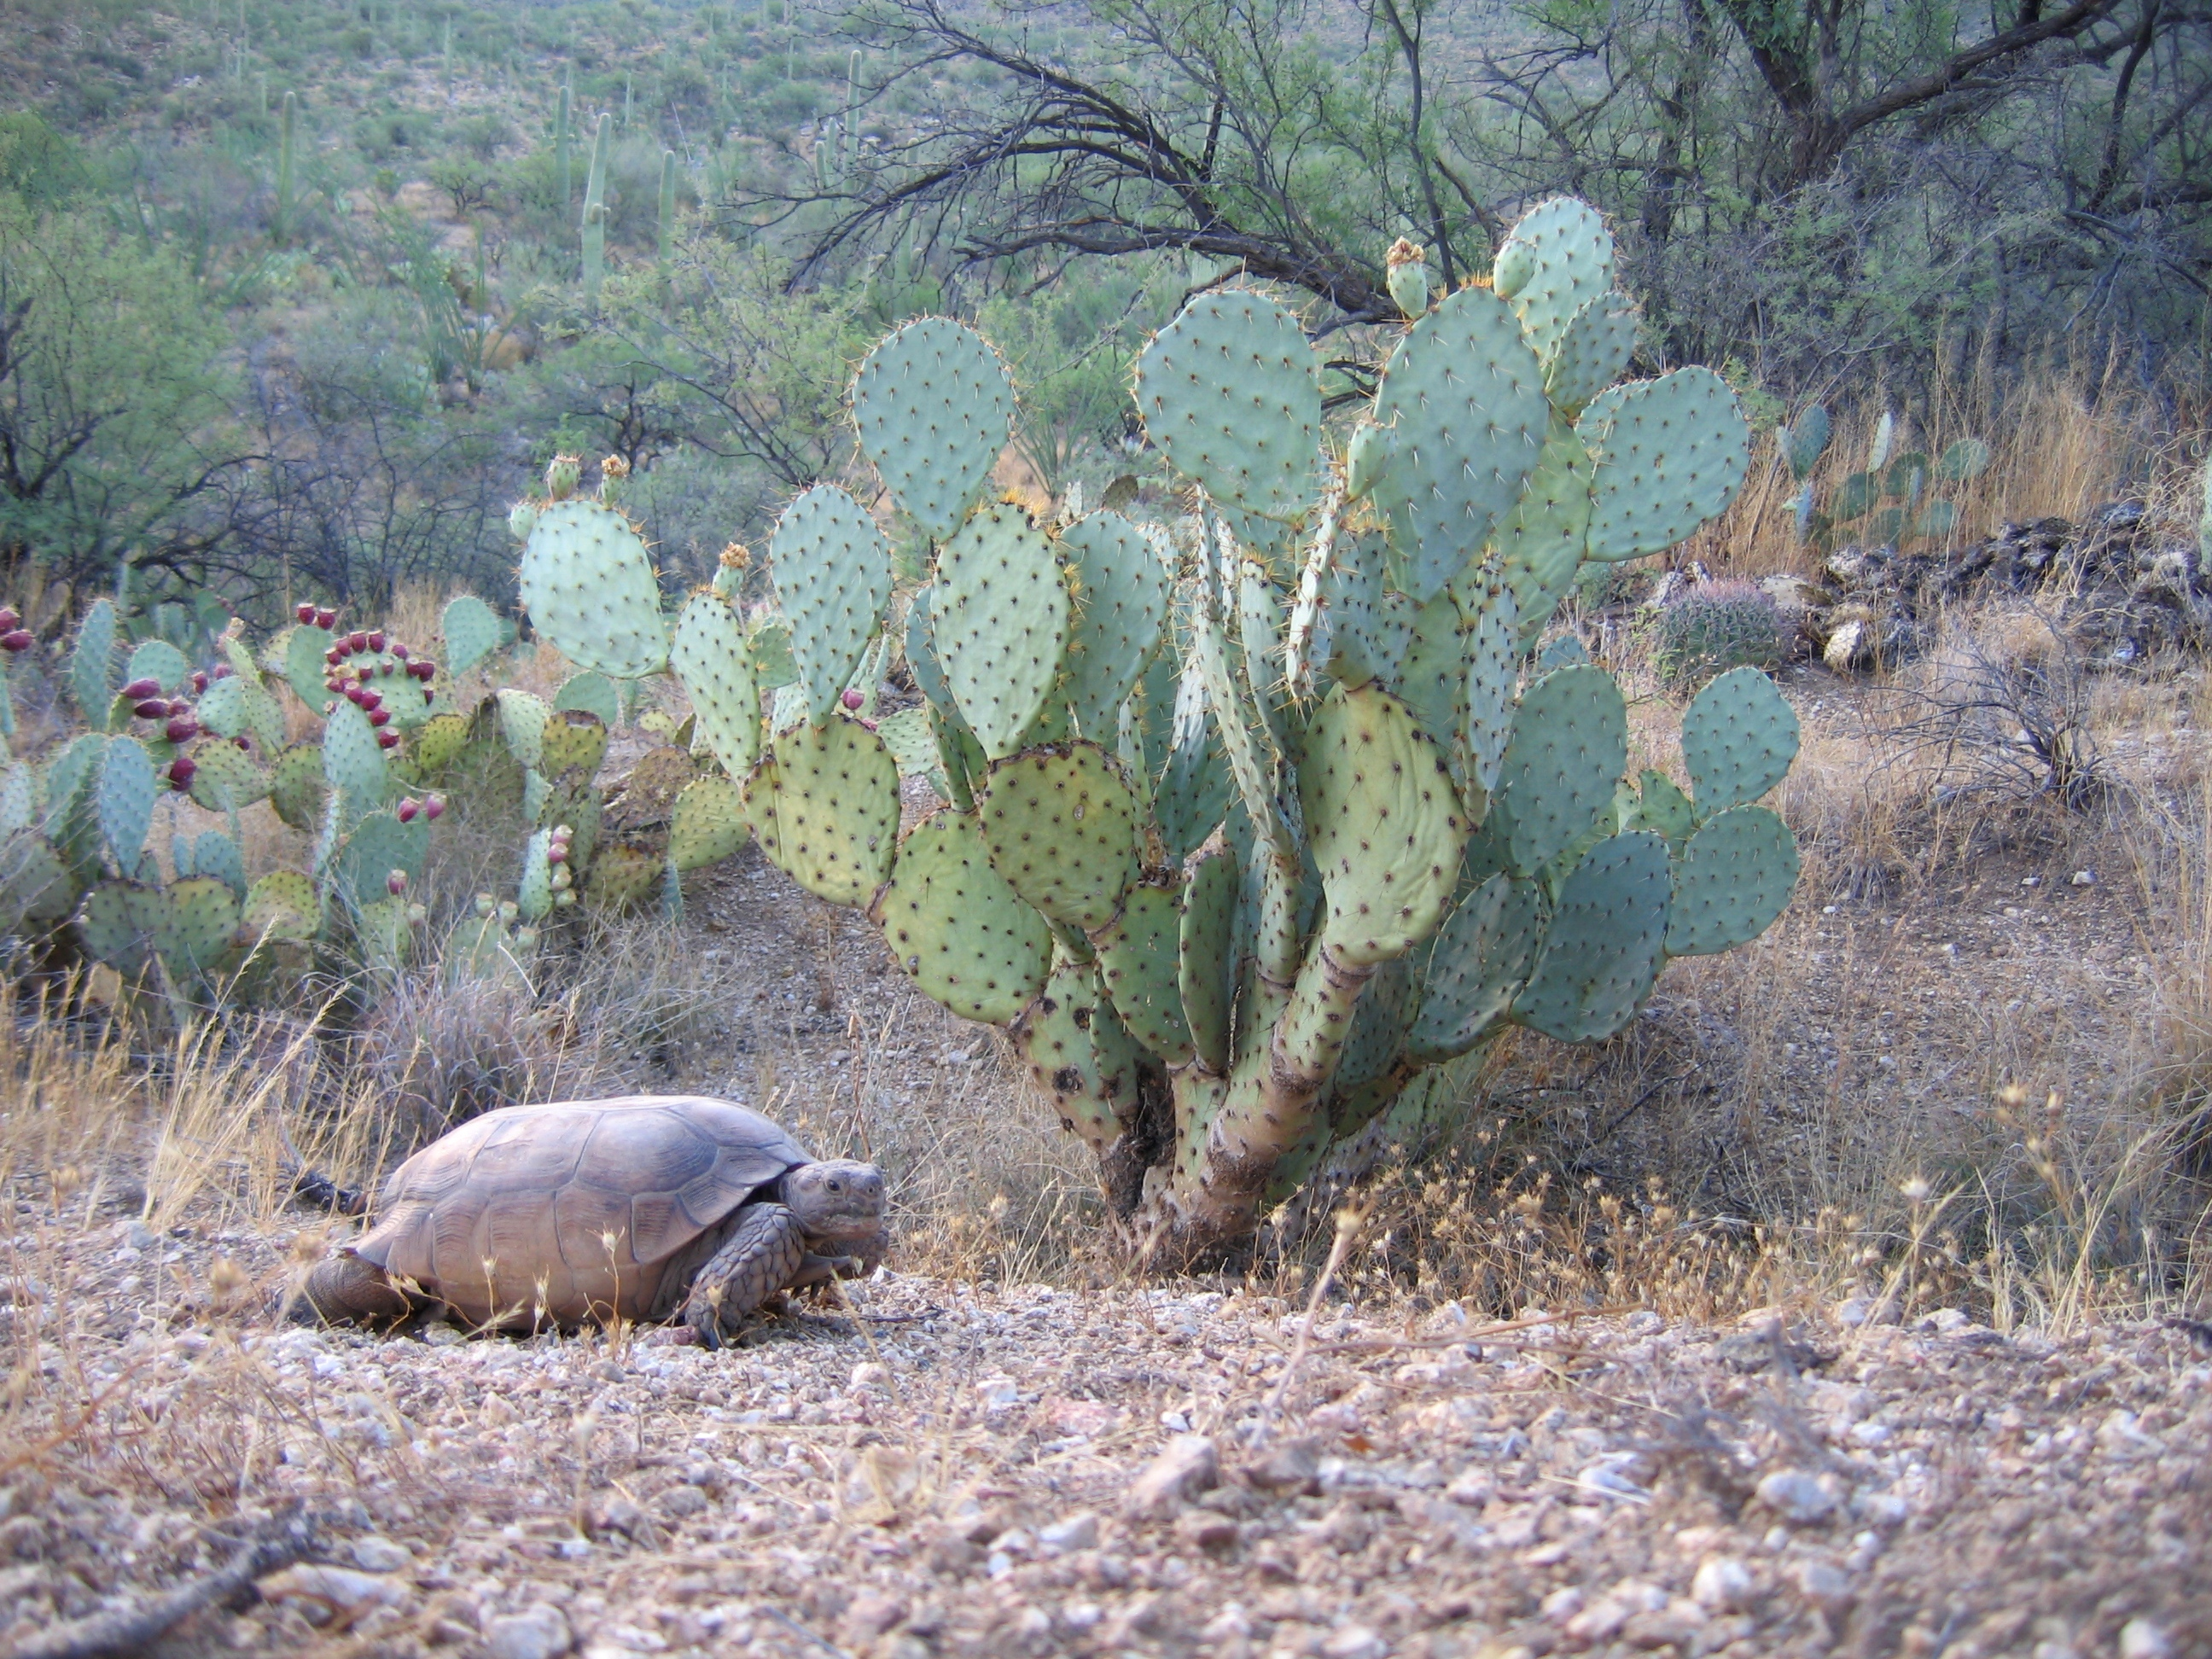
\includegraphics[height=3in,width=4in]{Ch3-Closed/figs/Erin_Zylstra_2.jpg}
\caption{Desert tortoise in its native habitat ({\it Photo credit: Erin
  Zylstra, Univ. of Arizona}).}
\label{closed.fig.tortoise}
\end{figure}

\begin{figure}[h]
\centering
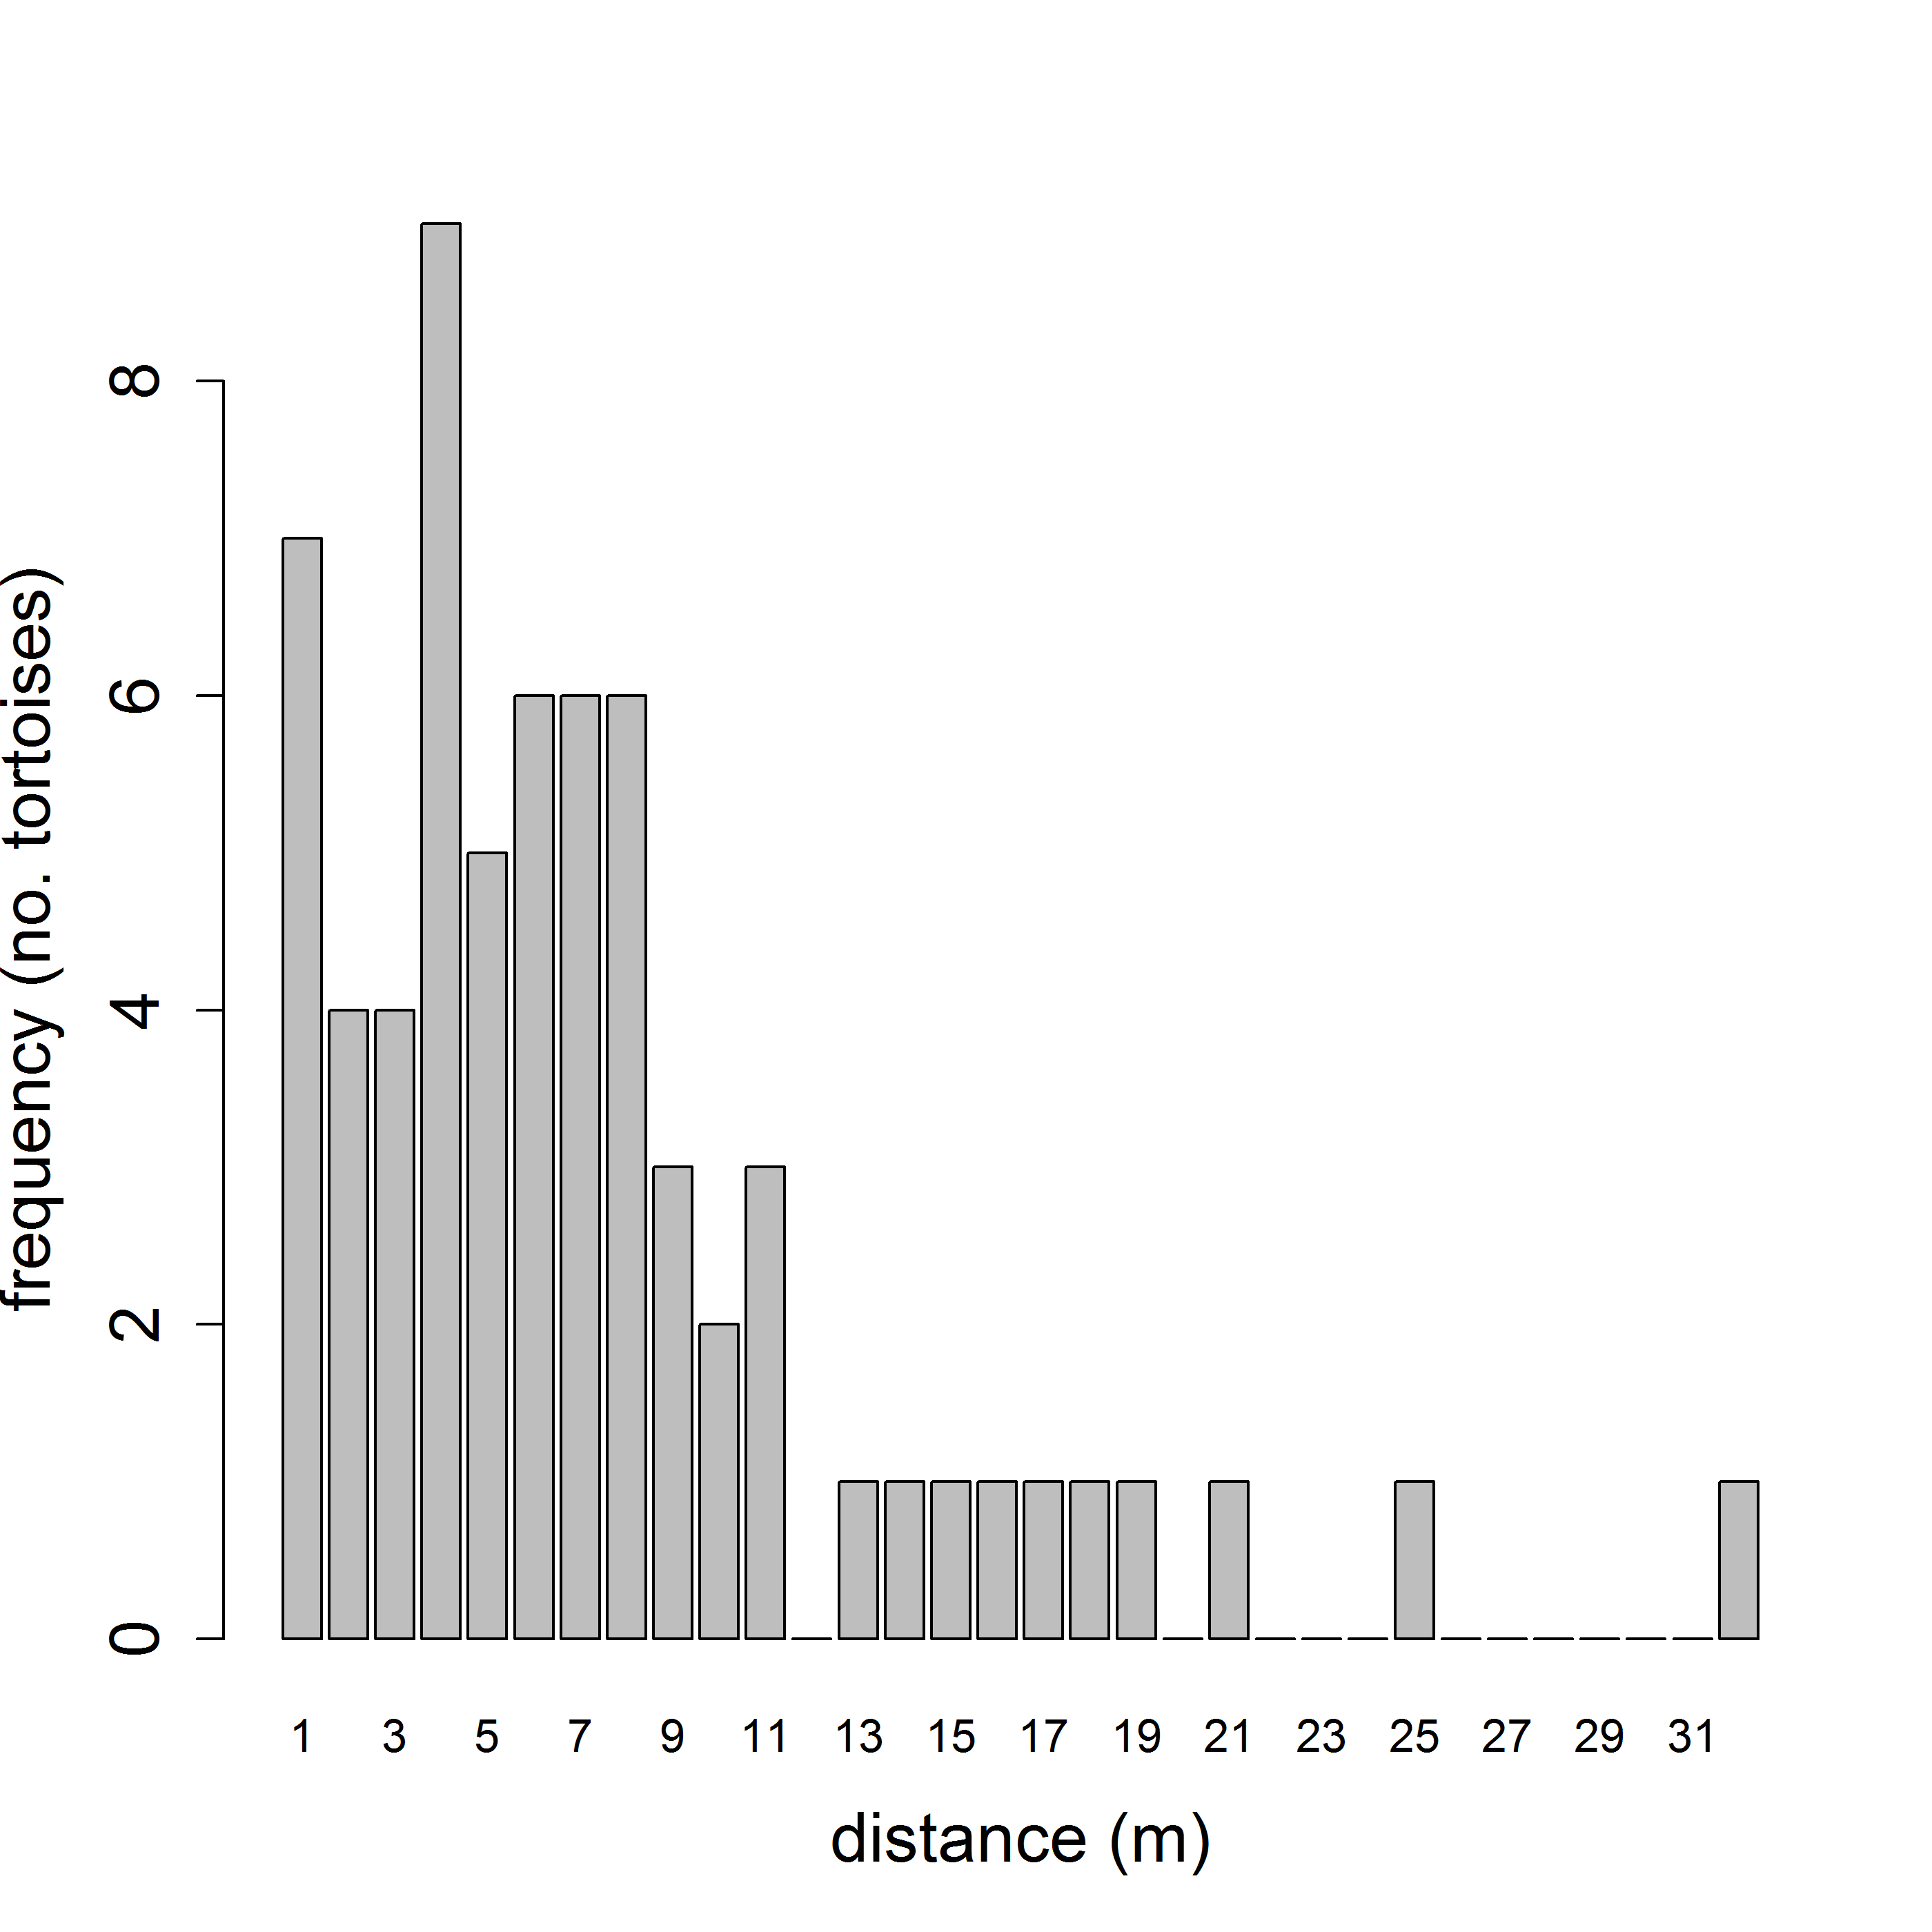
\includegraphics[height=3.0in,width=3.0in]{Ch3-Closed/figs/tortoise.png}
\caption{
Distance histogram of Sonoran desert tortoise detections from 120 km of
survey transect. }
\label{closed.fig.tortoisehist}
\end{figure}

Commands for reading in and organizing the data for analysis using {\bf
  WinBUGS}, followed by writing the model to a text file, are given
below. Note that the total sampled area of the transects \mbox{\tt
  striparea} is input as data, and computed as: $120$ (transects)
multiplied by the length ($1000$ m) and width ($B=40$ m), then
multiplied by 2, and then divided by $10000$ to convert to
units of individuals per ha. The full script is provided with the
\mbox{\tt scrbook} {\bf R} package (see \mbox{\tt ?tortoise}), where  we also give some commands for
analyzing the data with \mbox{\tt unmarked}
\citep{fiske_chandler:2011} using hierarchical distance sampling
models \citep{royle_etal:2004}.  
{\small
\begin{verbatim}
data(toroise)
x<-tortoise[,"Dist"]
nind<-sum(!is.na(x))

y<-rep(1,nind)        # create encounter vector
nz<-700               # data augmentation
y<-c(y,rep(0,nz))     # add 0s to the encounter vector
x<-c(x,rep(NA,nz))    # pad distance vector with NA
z<-y                  # starting vals for data augmentation variables

cat("
model{
alpha1~dunif(0,10)
sigma<- sqrt(1/(2*alpha1))
psi~dunif(0,1)

for(i in 1:(nind+nz)){
   z[i]~dbern(psi)      # DA Variables
   x[i]~dunif(0,B)      # B=strip width
   p[i]<-exp(logp[i])   # DETECTION MODEL
   logp[i]<-   -alpha1*(x[i]*x[i])
   mu[i]<-z[i]*p[i]
   y[i]~dbern(mu[i])    # OBSERVATION MODEL
 }

N<-sum(z[1:(nind+nz)])
D<- N/striparea  # area of transects
}
",file="dsamp.txt")
\end{verbatim}
}
After creating the model file, next 
we bundle the data,
provide initial values, indicate which parameters to monitor, and then
pass those things to {\bf WinBUGS}:
{\small
\begin{verbatim}
library(R2WinBUGS)

# density to be reported in units of ind/ha
data<-list(y=y,x=x,nz=nz,nind=nind,B=40,striparea=(120*1000*40*2/10000))
params<-list('alpha1','sigma','N','D','psi')
inits =  function() {list(z=z, psi=runif(1), alpha1=runif(1,0,.02) )}
fit = bugs(data, inits, params, model.file="dsamp.txt",working.directory=getwd(),
       debug=FALSE, n.chains=3, n.iter=3000, n.burnin=1000, n.thin=2)
\end{verbatim}
}
Posterior summaries for the tortoise data are given in Tab. \ref{closed.tab.dsamp}.
Estimated density (posterior mean) is $0.54$ individuals 
  per ha and the estimated scale parameter of the distance function
(posterior mean) is $\sigma=9.12$ meters.  The Rhat statistics of
around $1.02$ suggest that slightly longer MCMC simulations might be
useful. The posterior mass of the data augmentation parameter $\psi$
is located away from the upper-bound $\psi=1$ and so the degree of
data augmentation appears sufficient.

\begin{table}[ht]
  \caption{
    Posterior summaries from the tortoise distance sampling data. Results
    were obtained using {\bf WinBUGS}
    running
    3 chains, each with 3000 iterations and the first 1000 discarded,
    thinning by 2.
  }
\begin{tabular}{crrrrrrr} \hline \hline
 parameter &mean &   sd  & 2.5\%   &  50 \%  &   97.5\% &Rhat& n.eff
 \\ \hline
$\alpha_1$ &  0.01&  0.00 &   0.00 &  0.01   &   0.01 &1.02&   130   \\
$\sigma$  &   9.12&  0.77 &   7.77 &   9.07  &  10.77& 1.02&   130  \\
$N$       & 516.67& 54.71 & 415.00 & 516.00  & 632.00& 1.02&   100  \\
$D$       &   0.54&  0.06 &  0.43  & 0.54    &   0.66 &1.02&   100 \\
$\psi$    &   0.61&  0.07 &  0.49  & 0.61    &   0.75 &1.02&    96  \\ \hline
\end{tabular}
\label{closed.tab.dsamp}
\end{table}


\section{Summary and Outlook}

Traditional closed population capture-recapture models are closely
related to binomial generalized linear models.  Indeed, the only real
distinction is that in capture-recapture models, the population size
parameter $N$ (corresponding also to the size of a hypothetical
``complete'' data set) is unknown.  This requires special
consideration in the analysis of capture-recapture models. The
classical approach to inference recognizes that the observations don't
have a standard binomial distribution but, rather, a truncated
binomial (from which which the so-called {\it conditional likelihood}
derives) since we only have encounter frequency data on observed
individuals. If instead we analyze the models using data augmentation,
which arises under a $\mbox{Uniform}(0,M)$ prior for $N$, 
the observations can be modeled using a zero-inflated binomial
distribution. When we deal with the unknown-$N$ problem using
data augmentation then we are left with zero-inflated GLM and GLMMs
instead of ordinary GLM or GLMMs. The analysis of such zero-inflated
models is practically convenient, especially using the 
{\bf BUGS} variants.

Spatial capture-recapture models that we will consider in the rest of
the chapters of this book are closely related to 
individual covariate models. Heuristically, spatial capture-recapture
models arise by defining individual covariates based on observed
locations of individuals---we can think of using some function of
mean encounter location as an individual covariate. We did this in a
novel way, by using distance to the centroid of the trapping array as
a covariate. We analyzed the {\it full likelihood} using data
augmentation, and placed a prior distribution on the individual
covariate which was derived from an assumption that individual
locations are, a priori, uniformly distributed in space. This
assumption provides for invariance of the density estimator to the
choice of population size area (induced by maximum distance from the
centroid of the trap array). The model addressed some important problems in the
use of closed population models: it allows for heterogeneity in
encounter probability due to the spatial context of the problem and it
also provides a direct estimate of density because area is a feature
of the model (via the prior on the individual covariate). The model is
still not completely general because it does not make use of
the fully spatial encounter histories, which provide direct
information about the locations and density of individuals.  A
specific individual covariate model that is in widespread use is
classical distance sampling. The model underlying distance
sampling is precisely a special kind of SCR model---but one without
replicate samples. Understanding distance sampling and individual
covariate models more broadly provides a solid basis for understanding
and analyzing spatial capture-recapture models.


%\chapter{Closed population models}
%\label{chapt.closed}

\begin{comment}
\chapter{Fully Spatial Capture-Recapture Models}
\label{chapt.scr0}

%%%% TO DO  as of 12/29/11

 %%% Spell check document
 %%% ?all-zero? should be all-zero and not all zero ?all zero? ?all 0? etc..
 %%% Fix up R scripts and consolidate for R package
 %%% R commands to process wolverine data need included in that section

 %%% Run Wolverine 2k 4k and 8k grids in JAGS compare to WinBUGS
 %%%     insert those results in text

 %%%  For discrete state-space stuff, convert BUGS output to JAGS and
 %%%  figure out MC errors
 %%% Finish Table that has those results in it



\chapter{Fully Spatial Capture-Recapture Models}
\markboth{Chapter 4 }{}
\label{chapt.scr0}

\vspace{.3in}

In previous sections we discussed models that could be
viewed as primitive spatial capture-recapture models. We looked at a
basic distance sampling model and we also considered a classical
individual covariate modeling approach in which we defined a covariate
to be the distance from the (estimated) home range center to the center of
the trap array. These were spatial in the sense that they included
some characterization of where individuals live but, on the other
hand, only a primitive or no characterization of trap location.  That
said, there is only a small step from these two models to spatial
capture-recapture models that we consider in this chapter, which fully
recognize the spatial attribution of both individual animals {\it and}
the locations of encounter devices.

Fully spatial capture-recapture models must accommodate the spatial
organization of individuals and the encounter devices because the
encounter process occurs at the level of individual traps.  Failure to
consider the trap-specific data is the key deficiency
with classical ad-hoc approaches which aggregate encounter information
to the resolution of the entire trap array. We have  previously
addressed some problems that this induces including induced
heterogeneity in encounter probability, imprecise notation of ``sample
area'' and not being able to accommodate trap-specific
effects or trap-specific missing values.
In this chapter we resolve these issues by developing 
our first fully spatial capture-recapture
model which turns out to be precisely the model considered in sec. \ref{closed.sec.indcov},
 but instead of defining the individual covariate to be distance
to the centroid of the array we define $J$ individual covariates - the
distance to {\it each} trap. And, instead of using estimates of
individual locations ${\bf s}$, we consider a fully hierarchical model in
which we regard ${\bf s}$ as a latent variable and impose a prior
distribution on it.  We can think of having $J$ independent
capture-recapture studies generating one data set for each trap, and
applying the individual covariate model with random activity centers,
and that is all the basic SCR model is.

In the following sections of this chapter we investigate the basic
spatial capture-recapture model, which we refer to as ``model SCR0'',  and address some important
considerations related to its analysis in {\bf WinBUGS}. We also demonstrate
how to summarize posterior output for the purposes of producing
density maps or spatial predictions of density.

\section{Sampling Design and Data Structure}

In our development here, we will assume a standard sampling design in
which an array of $J$ traps is operated for $K$ time periods (say,
nights) producing encounters of $n$ individuals.  Because sampling
occurs by traps and also over time, the most general data structure
yields encounter histories for {\it each individual} that are
temporally {\it and} spatially indexed. Thus a typical data set will
include an encounter history {\it matrix} for each individual.  For
the most basic model, there are no time-varying covariates that
influence encounter, there are no explicit individual-specific
covariates, and there are no covariates that influence density. Hence, we will
develop models in this chapter for encounter data that are aggregated
over the temporal replicates. For example, suppose we observe 6
individuals in sampling at 4 traps over 3 nights of sampling then a
plausible data set is the $6 \times 4$ matrix of encounters, out of 3,
of the form:
\begin{verbatim}
      trap1 trap2 trap3 trap4
 [1,]     1     0     0     0
 [2,]     0     2     0     0
 [3,]     0     0     0     1
 [4,]     0     1     0     0
 [5,]     0     0     1     1
 [6,]     1     0     1     0
\end{verbatim}

We develop models in this chapter for passive detection 
devices such as ``hair snares''
or other DNA sampling methods \citep{kery_etal:2010,
  gardner_etal:2010jwm} and related types of sampling devices in which
(i) devices (effective ``traps'') may capture any number of individuals (i.e.,
they don't fill up; \begin{comment}
This is referred to as a ``multi-catch'' type of
sampling \citep{efford_etal:2009ecol})\end{comment}; (ii) an individual may be
captured in more than one trap during each occasion but (iii) 
individuals can be encountered at most 1 time by each trap during any
occasion.  Hair snares for sampling DNA from bears and other species
function according to these rules. An individual bear wandering about
its territory might come into contact with  $>1$ devices; A device may
encounter multiple bears; However, generally speaking, it will not be
possible to attribute multiple visits of the same individual to
distinct encounter events.

The statistical assumptions are that individual encounters
within and among traps are independent, and this allows us to regard
individual- and trap-specific encounters as {\it independent} Bernoulli trials
(see next section).  These basic (but admittedly at this point
somewhat imprecise) assumptions define the basic spatial
capture-recapture model, which we will refer to as ``SCR0'' 
so that we may use that model as a point of reference without having
to provide a long-winded enumeration of assumptions and sampling
design each time we do. We will make things more precise as we develop
a formal statistical definition of the model shortly.

While the model is most directly relevant
to hair snares and other DNA sampling methods for which multiple
detections of an individual are not distinguishable,
we will also make use of the model for data that arise from
camera-trapping studies. In practice, with camera trapping,
individuals might be photographed several times in a night but it is
common to 
 distill such data into a single binary encounter event for
reasons discussed later in Chapt. \ref{chapt.poisson-mn}.


\section{The binomial observation model }

If sampling devices are operated over $K$ time periods or sampling
occasions (e.g., in practice,
nights), and we assume that individual encounters are independent
across the $K$ sampling occasions, so that   
 individual and trap-specific encounters, $y_{ij}$,
are mutually independent outcomes of a binomial random variable:
\begin{equation}
	y_{ij} \sim \mbox{Bin}(K, p_{ij})
\label{scr0.eq.bin}
\end{equation}
This is the basic model underlying logistic regression (Chapt. \ref{chapt.glms})
as well as standard closed population models
(Chapt. \ref{chapt.closed}). The key
element of the model is that the encounter probability $p_{ij}$
depends 
on  both individual and trap. In a sense,
then, we can think of each {\it trap} as producing individual level
encounter history data of the classical variety - an $\mbox{\tt nind}
\times \mbox{\tt nreps}$
matrix of 0's and 1's (this is the ``encountered at most 1 time''
assumption).


As we did in sec. \ref{closed.sec.indcov}, we will make explicit the notion that
$p_{ij}$ is defined conditional on {\it where}  individual $i$
lives. Naturally, we think about defining an individual home range and
then relating $p_{ij}$ explicitly to the centroid of the individuals
home range, or its center of activity \citep{efford:2004,
  borchers_efford:2008, royle_young:2008}.  Therefore, define ${\bf
  s}_{i}$, a two-dimensional spatial coordinate, to be the activity
center for individual $i$. Then, the SCR model postulates that
encounter probability, $p_{ij}$, is a decreasing function
of distance between ${\bf s}_{i}$ and the location of trap $j$, ${\bf x}_{j}$.
 Naturally, if we think of modeling binomial counts using
logistic regression, we think about specifying the model according to:
\begin{equation}
	\mbox{logit}(p_{ij}) = \alpha_{0} + \alpha_1 ||{\bf s}_{i}-{\bf x}_{j} ||
\label{scr0.eq.logit}
\end{equation}
where, here, $||{\bf s}_{i}-{\bf x}_{j}||$ is the distance between
${\bf s}_{i}$ and ${\bf x}_{j}$. We sometimes write $||{\bf
  s}_{i}-{\bf x}_{j}|| = dist({\bf s}_{i},{\bf x}_{j}) =
d_{ij}$. Alternatively, if we think about distance sampling then we
might use the a model of the form:
\[
p_{ij} = p_{0}*\exp(-\alpha_{1} *||{\bf s}_{i}-{\bf x}_{j}||^2)
\]
which is usually referred to as the ``half-normal'' model in distance
sampling literature. Because it is the kernel of a bivariate normal or
Gaussian probability
density function we will refer to it as the ``(bivariate) normal'' or
``Gaussian'' model. 
There are a large number of standard detection models 
commonly used, and we consider these in
Chapt. \ref{chapt.covariates}).
Note that the bivariate normal model is equivalently represented as 
\begin{equation}
\log(p_{ij})  = \log(p_{0}) - \alpha_{1} *||{\bf s}_{i}-{\bf x}_{j}||^2
\label{scr0.eq.norm}
\end{equation}
which we make use of sometimes in specifying the model in the \bugs language. 
%We would always like to be clear that encounter probability depends on individual activity
%centers {\it and} trap locations {\it and} parameter(s) $\theta$, and
%so it would be ideal to write $p({\bf s}_{i},{\bf x}_{j}; \theta)$ or
%something similar. However, this can be extremely unwieldy and
%clutter up what are otherwise extremely simple mathematical
%expressions and formulae. As such, we will usually abbreviate these
%various dependencies by writing $p_{ij}$ or sometimes $p_{\theta,ij}$,
%understanding that $p_{ij}$ is actually a function of the various important
%quantities.
We probably expect that the parameter $\alpha_{1}$ in
Eq. \ref{scr0.eq.logit} or \ref{scr0.eq.norm} should be negative, so
that the probability of encounter decreases with distance between the
trap and individual home range center.  
Whatever model we choose for encounter probability, we should always keep
in mind that the model is described conditional on ${\bf s}_{i}$,
which is an unobserved random variable.  Thus, to be precise about
this, we should write the observation model as
\[
y_{ij}|{\bf s}_{i} \sim \mbox{Bin}(K, p({\bf s}_{ij};\alpha_{1}))
\]


The joint likelihood for the
data, conditional on the collection of individual activity centers,
can therefore be expressed as
\[
{\cal L}(\alpha_{1} | \{ {\bf y}_{i},{\bf s}_{i} \}_{i=1}^{N})
 =  \prod_{i} \prod_{j} \mbox{Bin}(y_{ij}|p_{ij}(\alpha_{1}))
\]
If we switch the indices on the product operators, we recognize that SCR likelihood (conditional on ${\bf s}$) is the product of $J$
{\it independent} capture-recapture likelihoods - one for each trap.
However, the data have a distinct ``repeated measures'' type of structure, with
each of the $j$ likelihood contributions for each individual being
grouped by individual. Thus, we cannot analyze the model
meaningfully by $J$ trap-specific models. In classical repeated measures
types of models, we accommodate the group structure of the data using
random effects (random individual or group level variables). For SCR
models we take the same basic approach, which we develop subsequently.

\subsection{Distance as a latent variable}

If we knew precisely every ${\bf s}_{i}$ in the population (and population size $N$), then the model specified by eqs. \ref{scr0.eq.bin} and
\ref{scr0.eq.logit} would be just an ordinary logistic
regression-type of a model which we learned how to fit using
\winbugs
 previously (Chapt. \ref{chapt.glms}), with a covariate $d_{ij}$. However,
the activity centers are unobservable even in the best possible
circumstances. In that case, $d_{ij}$ is an unobserved variable,
as in classical random effects models. We need to therefore
extend the model to accommodate these random variables with an
additional model component. A standard, and perhaps not unreasonable,
assumption is the so-called ``uniformity assumption'' which is to say
that the ${\bf s}_{i}$ are uniformly distributed over space (the
obvious next question ``which space?'' is addressed below).  This
uniformity assumption amounts to a uniform prior distribution on ${\bf
  s}_{i}$, i.e., the pdf of ${\bf s}_{i}$ is constant, which we may
express
\begin{equation}
	\Pr({\bf s}_{i}) \propto \mbox{\tt const}
\label{scr0.eq.sprior}
\end{equation}
 As it turns out, this assumption is usually not precise
enough to fit SCR models in practice for reasons we discuss in the
following section.  We will give another way to represent this prior
distribution that is more concrete, but depends on specifying the
``state-space'' of the random variable ${\bf s}_{i}$. The term
state-space is a technical way of saying ``the space of all possible outcomes''.

To summarize the preceeding model developing, a basic SCR model is
defined by 3 essential components:
\begin{itemize}
\item[(1)] Observation model: $y_{ij}|{\bf s}_{i} \sim \mbox{Bin}(K, p_{ij})$
\item[(2)] Encounter probability model: $\mbox{logit}(p_{ij}) = \alpha_{0} +
  \alpha_{1}*||{\bf s}_{i}-{\bf x}_{j}||$
\item[(3)] Point process model: $\Pr({\bf s}_{i} ) \propto \mbox{\tt const}$
\end{itemize}
Therefore, the SCR model is little more than an ordinary
capture-recapture model for closed populations. It is such a model,
but augmented with a set of ``individual effects'', ${\bf s}_{i}$,
which relate some sense of individual location to encounter
probability. 

\section{ The Binomial Point-process Model}

The collection of individual activity centers ${\bf s}_{1},\ldots,
{\bf s}_{N}$ represents a realization of a {\it binomial point process}
\citep[][p. xyz]{illian_etal:2008}.  The binomial point process (BPP)
is analogous to a Poisson point process in the sense that it
represents a ``random scatter'' of points in space - except that the
total number of points is {\it fixed}, whereas, in a Poisson point
process, it is random (having a Poisson distribution).  As an example,
we show in Fig. \ref{scr0.fig.bpp} locations of 20 individual activity
centers (black dots) in relation to a grid of 25 traps. For a Poisson
point process the number of such points in the prescribed state-space
would be random whereas often we will simulate fixed numbers of
points, e.g., for evaluating the performance of procedures such as how
well does our estimator perform of $N=50$?
\begin{figure}
\begin{center}
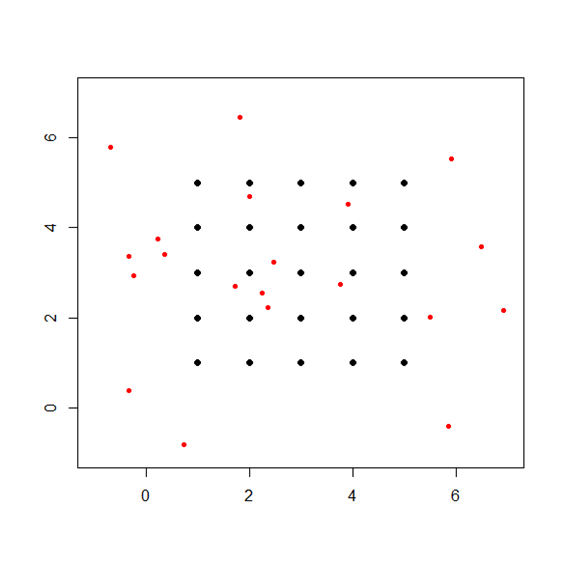
\includegraphics[height=2.5in]{Ch4/figs/binomialpoint}
\end{center}
\caption{Realization (small dots) of a binomial point process with $N=20$. The
  large dots represent trap locations.}
\label{scr0.fig.bpp}
\end{figure}

It is natural to consider a binomial point process in the context of
capture-recapture models because it preserves $N$ in the model and thus
preserves the linkage directly with closed population models. In fact,
under the binomial point process model, model $M_0$ and other closed
models are simple limiting cases of SCR models, i.e., as the
coefficient on distance ($\alpha_1$ above) tends to 0.
In addition, use of
the BPP model allows us to use data augmentation for Bayesian analysis
of the models as in Chapt. \ref{chapt.closed}, thus yielding a methodologically
coherent approach to analyzing the different classes of
models. Despite this, making explicit assumptions about $N$, such as
Poisson, is convenient in some cases (see Chapt. \ref{chapt.hscr}).

One consequence of having fixed $N$, in the BPP model, is that the
model is not strictly a model of ``complete spatial randomness''. This
is because if one forms counts $n(A_{1}),\ldots, n(A_{k})$ in any set
of disjoint regions say $A_{1}, \ldots, A_{k}$, then these counts are
{\it not} independent.  In fact, they have a multinomial distribution
\citep[see][p. 61]{illian_etal:2008}. Thus, the BPP model introduces
a slight bit of dependence in the distribution of points. However, in
most situations this will have no practical effect on any inference or
analysis and, as a practical matter, we will usually regard the BPP
model as one of spatial independence among individual activity centers
because each activity center is distributed independently of each
other activity center. Despite this implicit independence we see in
Fig. \ref{scr0.fig.bpp} that {\it realizations} of randomly distributed
points will typically exhibit distinct non-uniformity. Thus,
independent, uniformly distributed points will almost never appear
regularly, uniformly or systematically distributed. For this reason,
the basic binomial (or Poisson) point process models are enormously
useful in practical settings.  More relevant for SCR models is that we
actually have a little bit of data for some individuals and thus the
resulting posterior point pattern can deviate strongly from
uniformity, a point we come back to repeatedly in this book.
The uniformity hypothesis is only
a {\it prior} distribution which is directly affected by the quantity
and quality of the observed data, to produce a posterior distribution which
may appear distinctly non-uniform.


\subsection{Definition of home range center}

Some will be offended by our use of the concept of ``home range
center'' and question whether such notions as home ranges are useful
for some (or perhaps {\it any}) particular species.  Indeed, the idea
of a home range is a vague and purely phenomenological construct
anyway.  Despite this, it doesn't really matter whether or not a home
range makes sense for a particular species - individuals of any
species inhabit {\it some} region of space and we can define the
``home range center'' to be the center of the space that individual
was occupying (or using) during the period in which traps were
active. Thinking about it in that way, it could even be observable
(almost) as the centroid of a very large number of radio fixes over
the course of a survey period or a season.  Thus, this practical
version of a home range center in terms of space usage is a
well-defined construct regardless of whether one thinks the home range
itself is a meaningful concept, even if individuals are not
particularly territorial.  This is why we usually use the term
``activity center'' and we recognize that this is a transient thing
which applies only to a well-defined period of study.
%See sec. \ref{sec.scr0.implied} for more discussion of how to 
%interpret ${\bf s}$ in the context of the detection probability
%model. 


\subsection{The state-space of the point process}

Shortly we will focus on Bayesian analysis of this model with $N$
known so that we can directly apply to this situation what we learned
in Chapt. \ref{chapt.glms}. To do this, we note that the individual
effects ${\bf s}_{i},\ldots, {\bf s}_{N}$ are unknown quantities and
we will need to be able to simulate each ${\bf s}_{i}$ in the
population from the posterior distribution.  It should be self-evident
that we cannot simulate the ${\bf s}_{i}$ unless we describe precisely
the region over which they are uniformly distributed. This is the
quantity referred to above as the state-space, denoted henceforth by
${\cal S}$, which is a region or a set of points comprising the
potential values of ${\bf s}_{i}$. Thus, an equivalent explicit
statement of the ``uniformity assumption'' is
\[
{\bf s}_{i} \sim \mbox{Unif}({\cal S})
\]
where ${\cal S}$ is a precisely defined region. e.g., in Fig. 
\ref{scr0.fig.bpp}, ${\cal S}$ is the square defined by $[-1,7] \times
[-1, 7]$. Thus each of the $N=20$ points were generated by randomly
selecting each coordinate on the line $[-1, 7]$. 


\subsubsection{Prescribing the state-space}

Evidently, we need to define the state-space, ${\cal S}$. How can we
possibly do this objectively? Prescribing any particular ${\cal S}$
seems like the equivalent of specifying a ``buffer'' which we
criticized previously as being ad hoc. How is it, then, that the choice of a
state-space is {\it not} ad hoc? As a practical matter, it turns out
that estimates of density are insensitive to choice of the
state-space. As we observed in Chapt. \ref{chapt.closed}, it is true that $N$ increases
with ${\cal S}$, but only at the same rate as the area of ${\cal S}$
increases under the
prior assumption of constant density. As a result, we say that density
is invariant to ${\cal S}$ as long as ${\cal S}$ is sufficiently
large. Thus, while choice of ${\cal S}$ is (or can be) essentially
arbitrary, once ${\cal S}$ is chosen, it defines the population being
exposed to sampling, which scales appropriately with the size of the
state-space.

For our simulated system developed previously in this chapter, we
defined the state-space to be a square within which our trap array was
centered. For many practical situations this might be an
acceptable approach to defining the state-space. We provide an example
of this in sec. \ref{scr0.sec.wolverine} below in which the trap array is
irregular and also situated within a realistic landscape that is
distinctly irregular.  In general, it is most practical to define the
state-space as a regular polygon (e.g., rectangle) containing the trap
array without differentiating unsuitable habitat. Although defining
the state-space to be a regular polygon has computational advantages
(e.g., we can implement this more efficiently in {\bf WinBUGS} and
cannot for irregular polygons), a regular polygon induces an apparent
problem of admitting into the state-space regions that are distinctly
non-habitat (e.g., oceans, large lakes, ice fields, etc.).  It is
difficult to describe complex sets in mathematical terms that can be
used in {\bf BUGS}. As an alternative, we can provide a
representation of the state-space as a discrete set of points (sec.
\ref{scr0.sec.discrete}), that will allow specific points to be deleted
or not depending on whether they represent habitat, or we can define
the state-space as an arbitrary  collection of polygons stored as a GIS
shapefile
which can be analyzed easily using MCMC
(see sec. \ref{mcmc.sec.state-space}), but not so easily in the {\bf
  BUGS} variants.  In what follows below we provide an
analysis of the camera data defining the state-space to be a regular
continuous polygon (a rectangle).


\subsection{Invariance and the state-space as a model assumption}
\label{scr0.sec.invariance}

We will assert for all models we consider in this book that density is
invariant to the size and extent of ${\cal S}$, if ${\cal S}$ is
sufficiently large, and as long 
as our model relating $p_{ij}$ to ${\bf  s}_{i}$ is a decreasing
function of distance.  
We can prove this easily by drawing an analogy with a 1-d case
involving 
 distance sampling.  Let $y_{j}$ be the number of individuals
captured in some interval $[d_{j-1},d_{j})$, and define $d_{J} = B$
for some large value of $B$.  
The observations from a survey are $y_{1},\ldots,y_J$ and the
likelihood is a multinomial likelihood, so the log-likelihood is of
the form
\[
logL(\{ y_{j} \}) = \sum_{j} y_{j=1}^{J} \pi_{j}
\]
where $\pi_{j}$ is the probability of detecting an individual in
distance class $j$, which depends on parameters of the detection
function (the manner of which is not relevant for the present
discussion).  For $B$ sufficiently large, we guarantee that $E[y_{J}]
= 0$ and therefore the observed frequency in the ``last cell''
contributes nothing to the likelihood, in regular situations in which
the detection function decays monotonically with distance and prior
density is constant.


Sometimes
our estimate of density can be affected by choosing ${\cal S}$ too
small. However, 
this might be sensible if ${\cal S}$ is naturally well-defined. As we discussed
in Chapt. \ref{chapt.intro}, {\bf choice of ${\cal S}$ is part of the
  model}, and thus it is sensible 
that estimates of density might be sensitive to its definition
  in problems where it is natural to restrict ${\cal S}$.
One could imagine,
however, that in specific cases where you're studying a small
population with well-defined habitat preferences, that a problem could
arise because changing the state-space around based on differing
opinions and GIS layers might have substantial changes on the density
estimates and hence those of 
population size. But this is a real biological problem and a natural
consequence of the spatial formalization of capture-recapture models -
a feature, not a bug or some statistical artifact - and it should be
resolved with better information, research, and thinking.
 For situations where there is not a natural
choice of ${\cal S}$, we should default to choosing ${\cal S}$ to be very large in order
to achieve invariance or, otherwise, evaluate sensitivity of density
estimates by trying a couple of different choices of ${\cal S}$. This is a
standard ``sensitivity to prior'' argument that Bayesians always have
to be conscious of.  We demonstrate this in our analysis of section
\ref{scr0.sec.wolverine}
below. As an additional practical 
consideration, we note that $area({\cal S})$ affects data augmentation. If you
increase $area({\cal S})$ then there are more individuals to account for and
therefore the size of the augmented data set $M$ must increase.

We have been told that one can carry-out non-Bayesian analyses of SCR
models without having to specify the state-space of the point process
or perhaps while only specifying it imprecisely.  This assertion is
incorrect. We assume people are thinking this because {\it they} don't
have to specify it explicitly because someone else has done it for
them in a package that does integrated likelihood. Even to do
integrated likelihood (see Chapt. \ref{chapt.mle}) we have to integrate the
conditional-on-${\bf s}$ likelihood over some 2-dimensional space.  It might
work that the integration can be done from $-\infty$ to $+\infty$ but
that is a mathematical artifact of specific detection functions, and
an implicit definition of a state-space that doesn't make biological
sense in any real context. %%%, even though it may in fact be innocuous.


\subsection{Connection to Model  $M_h$}  \label{scr0.sec.scrmh}

SCR models are closely related to heterogeneity models. In SCR models,
heterogeneity in encounter probability is induced by both the effect
of distance in the model for detection probability and also from
specification of the state-space. Hence, the state-space  is an
explicit element of the model. 
To understand this, suppose we have a random
effect with some prior distribution:
\[
{\bf s} \sim \mbox{Unif}({\cal S})
\]
and encounter probability is a function of ${\bf s}$, denoted by 
 $p({\bf s}) = p(y=1|{\bf s})$. 
For example, under Eq. \ref{scr0.eq.logit}
we have that 
\[
p({\bf s}) = logit^{-1} ( \alpha_{0} + \alpha_1 ||{\bf
  s}_{i}-{\bf x}_{j} || )
\]
and we can work out, either analytically or empirically, what is the
implied distribution of $p$ for a population of individuals.  We show
an illustration in Fig. \ref{scr0.fig.buffereffect} which shows a
histogram of $p$ for a hypothetical population of 100000 individuals
on a state-space enclosing our $5 \times 5$ trap array above, under
the logistic model for distance given by Eq. \ref{scr0.eq.logit}. {\bf
  R} code is provided in the {\bf R} package \mbox{\tt scrbook} to
produce this analysis for the logistic and half-normal models. The
histogram shows the encounter probability under buffers of 0.2, 0.5
and 1.0. We see the mass shifts to the left as the buffer increases,
implying more individuals with lower encounter probabilities, as their
home range centers increase in distance from the trap array.


\begin{figure}
\begin{center}
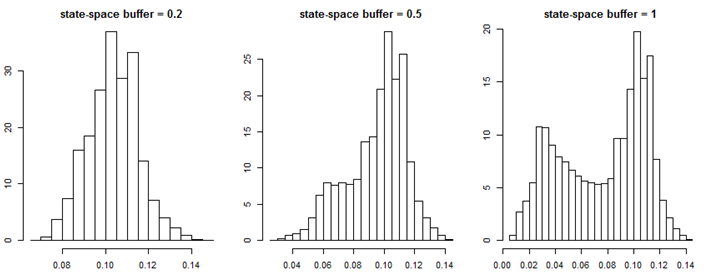
\includegraphics[width=5in]{Ch4/figs/buffereffect}
\end{center}
\caption{Implied population distribution of $p_{i}$ for a population
  of individuals as a function of the size of the state-space buffer
  around a trap array. The trap array is fixed and centered within a
  square state-space.}
xxxxxxxxxxxxxxx
$The main titles of the three panel plots are too small. I would rather call them (a), (b) and (c) and then give their associated information in the figure legend. Also, numbers on axes are very small for the sight of men in our age$ xxxxxxxxxxxxxxxxxxxx
\label{scr0.fig.buffereffect}
\end{figure}

Another way to understand this is by representing ${\cal S}$ as a set
of discrete points on a grid. In the coarsest possible case where
${\cal S}$ is a single arbitrary point, then every individual has
exactly the same $p$. As we increase the number of points in ${\cal
  S}$,  more distinct values of $p$ are possible. As such, when
${\cal S}$ is characterized by discrete points then SCR models are
precisely a type of finite-mixture model \citep{norris_pollock:1996,
  pledger:2000}, except, in the case of SCR models, we have some information about which
group an individual belong (i.e., where their activity center is), as
a result of their captures in traps.

This context suggests the problem raised by \citet{link:2003}. He
showed that in most practical situations $N$ may not be identifiable
across classes of mixture distributions which in the context of SCR
models is the pair $(g, {\cal S})$.  The difference, however, is that
we do obtain some direct information about ${\bf s}$ in SCR models and
therefore it may be reasonable to expect that
$N$ is identifiable across models characterized by $(g,{\cal
  S})$.

\subsection{Connection to Distance Sampling}

It is worth re-emphasizing that the basic SCR model is a binomial
encounter model in which distance is a covariate. As such, it is
strikingly similar to a classical distance sampling model \citep{buckland_etal:2002}. Both have
distance as a covariate but in classical distance sampling problems
the focus is on the distance between the observer and the animal at an
instant in time, not the distance between a trap and an animal's home
range center. As a practical matter, in distance sampling, ``distance'' is {\it
  observed} for those individuals that appear in the
sample. Conversely, in SCR problems, it is only imperfectly observed
(we have partial information in the form of trap observations).
Clearly, it is preferable to observe distance if possible, but 
distance sampling requires field methods that
are often not practical in many situations, e.g. when studying
carnivores such as bears or large cats. Furthermore, SCR models allow us to relax many of the
assumptions made in classical distance sampling, such as perfect detection at distance zero, and SCR models allow
for estimates of quantities other than density, such as home range
size, and space usage (see Chapts. XXXXX And \ref{chapt.ecoldist}).


\section{Simulating SCR Data}

It is always useful to simulate data because it allows you to
understand the system that you're modeling and also calibrate your
understanding with the parameter values of the model. That is, you can
simulate data using different parameter values until you obtain data
that ``look right'' based on your knowledge of the specific situation
that you're interested in. Here we provide a simple script to
illustrate how to simulate spatial encounter history data. In this
exercise we simulate data for 100 individuals and a 25 trap array laid
out in a $5 \times 5$ grid of unit spacing.  The specific encounter model is
the half-normal model given above and we used this code to simulate
data used in subsequent analyses.  The 100 activity centers were
simulated on a state-space defined by a $8 \times 8$ square within which the
trap array was centered (thus the trap array is buffered by 2
units). Therefore, the density of individuals in this system is fixed
at $100/64$.

{\small
xxxxxx$This is an example of a panel I like: The code is nicely laid out and well explained$xxxxxx
\begin{verbatim}
	set.seed(2013)
# create 5 x 5 grid of trap locations with unit spacing
traplocs<- cbind(sort(rep(1:5,5)),rep(1:5,5))
Dmat<-e2dist(traplocs,traplocs) 
ntraps<-nrow(traplocs)

# define state-space of point process. (i.e., where animals live).
# "delta" just adds a fixed buffer to the outer extent of the traps.
delta<-2
Xl<-min(traplocs[,1] - delta)
Xu<-max(traplocs[,1] + delta)
Yl<-min(traplocs[,2] - delta)
Yu<-max(traplocs[,2] + delta)

N<-100   # population size
K<- 20    # number nights of effort

sx<-runif(N,Xl,Xu)    # simulate activity centers
sy<-runif(N,Yl,Yu)
S<-cbind(sx,sy)
D<- e2dist(S,traplocs)  # distance of each individual from each trap

alpha0<- -2.5      # define parameters of encounter probability
sigma<- 0.5        #
alpha1<- 1/(2*sigma*sigma)
probcap<- plogis(-2.5)*exp( - alpha1*D*D)    # probability of encounter 
# now generate the encounters of every individual in every trap
Y<-matrix(NA,nrow=N,ncol=ntraps)
for(i in 1:nrow(Y)){
   Y[i,]<-rbinom(ntraps,K,probcap[i,])
}
\end{verbatim}
}

We remind the reader that, in presenting \R or other code snippets
throughout the book, we will deviate from our standard variable
expressions for some quantities. 
In particular, we sometimes 
substitute words for integer variable designations:
\mbox{\tt nind} (for $n$), \mbox{\tt ntraps} (for $J$), and \mbox{\tt
 nperiods} (for $K$). In our opinion this leaves less to be infereed
 in a \bugs model definition.

Subsequently we will generate data using this code packaged in an {\bf
  R}
function called \mbox{\tt simSCR0.fn} in the package \mbox{\tt
  scrbook} which takes a number of
arguments including \mbox{\tt discard0} which, if \mbox{\tt TRUE}, will return
only the encounter histories for captured individuals.  A second
argument is \mbox{\tt array3d} which, if \mbox{\tt TRUE}, returns the 3-d
encounter history array instead of the aggregated \mbox{\tt nind}
$\times \mbox{\tt ntraps}$ encounter frequencies (see below). Finally
we provide a random number seed, \mbox{\tt sd = 2013} to ensure
repeatability of the analysis here. We obtain a data set as above using the
following command:
\begin{verbatim}
data<-simSCR0.fn(discard0=TRUE,array3d=FALSE,sd=2013)
\end{verbatim}
The {\bf R} object \mbox{\tt data} is a list, so let's take a look at
what's in the list and then harvest some of its elements for further
analysis below.
{\small
\begin{verbatim}
> names(data)
[1] "Y"        "traplocs" "xlim"     "ylim"     "N"        "alpha0"   "beta"
[8] "sigma"    "K"
> Y<-data$Y
> traplocs<-data$traplocs
\end{verbatim}
}

\subsection{Formatting and manipulating real data sets}
\label{scr0.sec.formats}

Conventional capture-recapture data are easily stored and manipulated
as a 2-dimensional array, an $\mbox{\tt nind} \times \mbox{\tt
  nperiod}$ matrix, which is maximally informative for any
conventional capture-recapture model, but not for spatial
capture-recapture models.  For SCR models we must preserve the spatial
information in the encounter history information. We will routinely
analyze data from 3 standard formats:
\begin{itemize}
\item[(1)] The basic 2-dimensional data format, which is an \mbox{\tt
    nind} $\times$ \mbox{\tt ntraps} encounter frequency matrix such
  as that simulated previously. These are the total number of encounters in each
  trap, summed over replicate samples.
\item[(2)] The maximally informative 3-dimensional array, for which we
  establish here the convention that it has dimensions \mbox{\tt nind}
  $\times$ \mbox{\tt nperiods} $\times$ \mbox{\tt ntraps}.\item[(3)] We use a compact format - the ``SCR flat format'' - which
  we describe below in section \ref{scr0.sec.wolverine}.
\end{itemize}
To simulate data in the most informative format - the ``3-d array'' -
we can use the {\bf R} commands given previously but replace the last
4 lines with the following:
{\small
\begin{verbatim}
Y<-array(NA,dim=c(N,K,ntraps))
for(i in 1:nrow(Y)){
for(j in 1:ntraps){
 Y[i,1:K,j]<-rbinom(K,1,probcap[i,j])
}
}
\end{verbatim}
}
We see that a collection of $K$ binary encounter events are generated
for {\it each} individual and for {\it each} trap.  The probabilities
of those Bernoulli trials are computed based on the distance from
each individuals home range center and the trap (see calculation
above), and those are housed in the matrix \mbox{\tt probcap}. Our data simulator
function \mbox{\tt simSRC0.fn} will return the full 3-d array if
\mbox{\tt array3d=TRUE} is specified in the function call.  To recover
the 2-d matrix from the 3-d array, and subset the 3-d array to
individuals that were captured, we do this:
{\small
\begin{verbatim}
Y2d<- apply(Y,c(1,3),sum) # sum over the ``replicates'' dimension (2nd margin of the array)
ncaps<-apply(Y2d,1,sum)   # compute how many times each individual was captured
Y<-Y[ncaps>0,,]           # keep those individuals that were captured
\end{verbatim}
}

\section{Fitting an SCR Model in BUGS}
\label{scr0.sec.winbugs1}

Clearly if we somehow knew the value of $N$ then we could fit this
model directly because, in that case, it is a special kind of logistic
regression model - one with a random effect, but that enters into the
model in a peculiar fashion - and also with a distribution (uniform)
which we don't usually think of as standard for random effects models.
So our aim here is to analyze the known-$N$ problem, using our
simulated data, as an incremental step in our progress toward fitting
more generally useful models.

To begin, we use our simulator to grab a data set and then harvest the
elements of the resulting object for further analysis.
\begin{verbatim}
data<-simSCR0.fn(discard0=FALSE,sd=2013)
y<-data$Y
traplocs<-data$traplocs
nind<-nrow(y)
X<-data$traplocs
J<-nrow(X)
y<-rbind(y,matrix(0,nrow=(100-nrow(y)),ncol=J ) )
Xl<-data$xlim[1]
Yl<-data$ylim[1]
Xu<-data$xlim[2]
Yu<-data$ylim[2]
\end{verbatim}

Note that we specify \mbox{\tt discard0 = FALSE} so that we have a
"complete" data set, i.e., one with the all-zero encounter histories
corresponding to uncaptured individuals. Now, within an {\bf R} session, we
can create the {\bf BUGS} model file and fit the model using the following
commands. 
{\small
\begin{verbatim}
cat("
model {
alpha0~dnorm(0,.1)
logit(p0)<- alpha0
alpha1~dnorm(0,.1)
for(i in 1:N){
   s[i,1]~dunif(Xl,Xu)
   s[i,2]~dunif(Yl,Yu)    
for(j in 1:J){
d[i,j]<- pow(pow(s[i,1]-X[j,1],2) + pow(s[i,2]-X[j,2],2),0.5)
y[i,j] ~ dbin(p[i,j],K)
p[i,j]<- p0*exp(- alpha1*d[i,j]*d[i,j])
}
}

}
",file = "SCR0a.txt")
\end{verbatim}
}
This model describes the half-normal detection model but it
would be trivial to modify that to various others including the
logistic described above. One consequence of using the half-normal is
that we have to constrain the encounter probability to be in $[0,1]$
which we do here by defining \mbox{\tt alpha0} to be the logit of the
intercept parameter \mbox{\tt p0}. Note that the distance covariate is
computed within the {\bf BUGS} model specification given the matrix of trap
locations, \mbox{\tt X}, which is provided to {\bf WinBUGS} as data.

Next we do a number of organizational activities including bundling
the data for {\bf WinBUGS}, defining some initial values, the parameters to
monitor and some basic MCMC settings.  We choose initial values for
the activity centers ${\bf s}$ by generating uniform random numbers in
the state-space but, for the observed individuals, we replace those
values by each individual's mean trap coordinate for all encounters
{\small
\begin{verbatim}
sst<-cbind(runif(nind,Xl,Xu),runif(nind,Yl,Yu))  # starting values for s
for(i in 1:nind){
if(sum(y[i,])==0) next
sst[i,1]<- mean( X[y[i,]>0,1] )
sst[i,2]<- mean( X[y[i,]>0,2] )
}

data <- list (y=y,X=X,K=K,N=nind,J=J,Xl=Xl,Yl=Yl,Xu=Xu,Yu=Yu)
inits <- function(){
  list (alpha0=rnorm(1,-4,.4),alpha1=runif(1,1,2),s=sst)
}

library("R2WinBUGS")
parameters <- c("alpha0","alpha1")
nthin<-1
nc<-3
nb<-1000
ni<-2000
out <- bugs (data, inits, parameters, "SCR0a.txt", n.thin=nthin,
n.chains=nc, n.burnin=nb,n.iter=ni,debug=TRUE,working.dir=getwd())
\end{verbatim}
}
There is little to say about the preceding basic operations other than
to suggest that the interested reader explore the output and
additional analyses by running the script provided in the {\bf R}
package \mbox{\tt scrbook}.
 We ran $1000$ burn-in and $1000$ after burn-in, 3 chains,
to obtain 3000 posterior samples.  Because we know $N$ for this
particular data set we only have 2 parameters of the detection model
to summarize (\mbox{\tt alpha0} and \mbox{\tt alpha1}).  When the
object \mbox{\tt out} is produced we print a summary of the results as
follows:
{\small
\begin{verbatim}
> print(out,digits=3)
Inference for Bugs model at "SCR0a.txt", fit using WinBUGS,
 3 chains, each with 2000 iterations (first 1000 discarded)
 n.sims = 3000 iterations saved
            mean     sd    2.5%     25%    50%     75%   97.5%  Rhat n.eff
alpha0    -2.496  0.224  -2.954  -2.648  -2.48  -2.340  -2.091 1.013   190
alpha1     2.442  0.419   1.638   2.145   2.44   2.721   3.303 1.005   530
deviance 292.803 21.155 255.597 277.500 291.90 306.000 339.302 1.006   380
.
 [some output deleted]
.
\end{verbatim}
}

We know the data were generated with \mbox{\tt alpha0} $= -2.5$ and
\mbox{\tt alpha1 = -2}. The estimates look reasonably close to those
data-generating values and we probably feel pretty good about the
performance of the Bayesian analysis and MCMC algorithm that {\bf WinBUGS}
cooked-up based on our sample size of 1 data set.  It is worth noting
that the Rhat statistics indicate reasonable convergence but, as a
practical matter, we might choose to run the MCMC algorithm for
additional time to bring these closer to 1.0 and to increase the
effective posterior sample size (\mbox{\tt n.eff}). Other summary output includes
``deviance'' and related things including the deviance information
criterion (DIC). We discuss these things in Chapts. \ref{chapt.mcmc}
and \ref{chapt.gof}.



\section{Unknown N}
\label{scr0.sec.unknownN}

In all real applications $N$ is unknown and that fact is kind of an
important feature of the capture-recapture problem!  We handled this
important issue in Chapt. \ref{chapt.closed} using the method of data augmentation
which we apply here to achieve a realistic analysis of model SCR0. As
with the basic closed population models considered previously, we
formulate the problem here by augmenting our observed data set with a
number of ``all-zero'' encounter histories - what we referred to in
Chapt. \ref{chapt.closed} as potential individuals. If $n$ is the number of observed
individuals, then let $M-n$ be the number of potential individuals in
the data set. For the basic $y_{ij}$ data structure (individuals x
traps encounter frequencies) we simply add additional rows of all-zero
observations to that data set. This is because such
``individuals'' are unobserved, and therefore necessarily have
$y_{ij}=0$ for all $j$.  A data set, say with 4 traps and 6 individuals,
augmented with 4 pseudo-individuals therefore might look like this:
{\small
\begin{verbatim}
      trap1 trap2 trap3 trap4
 [1,]     1     0     0     0
 [2,]     0     2     0     0
 [3,]     0     0     0     1
 [4,]     0     1     0     0
 [5,]     0     0     1     1
 [6,]     1     0     1     0
 [7,]     0     0     0     0
 [8,]     0     0     0     0
 [9,]     0     0     0     0
[10,]     0     0     0     0
\end{verbatim}
}
We typically have more than 4 traps and, if we're fortunate, many more
individuals in our data set.

For the augmented data, we introduce a set of binary latent variables
(the data augmentation variables), $z_{i}$, and the model is extended
to describe $\Pr(z_{i} = 1)$ which is, in the context of this problem,
the probability that an individual in the augmented data set is a
member of the population that was sampled. In other words, if $z_{i}=1$
for one of the all-zero encounter histories, this is implied to be
a sampling zero whereas observations for which $z_{i}=0$ are
``structural zeros'' under the model.

How big does the augmented data set have to be? We discussed this
issue in Chapt. \ref{chapt.closed} where we noted that the size of the data set is
equivalent to the upper limit of a uniform prior distribution on $N$.
Practically speaking, it should be sufficiently large so that the
posterior distribution for $N$ is not truncated. On the other hand, if
it is too large then unnecessary calculations are being done. An
approach to choosing $M$ by trial-and-error is indicated. You can take
a ballpark estimate of the probability that an individual is captured
at all during the study, say $\tilde{p}$, which is related to the
``per sample'' encounter probability, $p$, by $\tilde{p} = 1-(1-p)^{K}$, obtain $N$ as $n/\tilde{p}$, and then set $M =
2*N$, as a first guess. Do a short MCMC run and then consider whether
you need to increase $M$. See Chapt. \ref{chapt.mcmc} for an
example of this. \citet[][ch. 6]{kery_schaub:2011}
 provide an assessment of choosing $M$ in closed population models.

Analysis by data augmentation removes $N$ as an explicit parameter of
the model. Instead, $N$ is a derived parameter, computed by $N=
\sum_{i=1}^{M} z_{i}$. Similarly, {\it density}, $D$, is also a
derived parameter computed as $D=N/area({\cal S})$. For our
simulator, we're using an $8 \times 8$ state-space and thus we will
compute $D$ as $D=N/64$.

\subsection{Analysis using data augmentation in WinBUGS}

As before we begin by obtaining a data set using our \mbox{\tt
  simSCR0.fn} routine and then harvesting the required data objects
from the resulting data list.  Note that we use the \mbox{\tt
  discard0=TRUE} option this time so that we get a ``real'' data set
with no all-zero encounter histories. After harvesting the data we
produce the {\bf WinBUGS} model specification which now includes $M$
encounter histories including the augmented potential individuals, the
data augmentation parameters $z_{i}$, and the data augmentation
parameter $\psi$.
{\small
\begin{verbatim}
data<-simSCR0.fn(discard0=TRUE,sd=2013)
y<-data$Y
traplocs<-data$traplocs
nind<-nrow(y)
X<-data$traplocs
J<-nrow(X)
Xl<-data$xlim[1]
Yl<-data$ylim[1]
Xu<-data$xlim[2]
Yu<-data$ylim[2]

cat("
model {
alpha0~dnorm(0,.1)
logit(p0)<- alpha0
alpha1~dnorm(0,.1)
psi~dunif(0,1)

for(i in 1:M){    
   z[i] ~ dbern(psi)
   s[i,1]~dunif(Xl,Xu)
   s[i,2]~dunif(Yl,Yu)
   for(j in 1:J){
      d[i,j]<- pow(pow(s[i,1]-X[j,1],2) + pow(s[i,2]-X[j,2],2),0.5)
      y[i,j] ~ dbin(p[i,j],K)
      p[i,j]<- z[i]*p0*exp(- alpha1*d[i,j]*d[i,j])
   }
}
N<-sum(z[])
D<-N/64
}
",file = "SCR0a.txt")
\end{verbatim}
}

To prepare our data we have to augment the data matrix \mbox{\tt y}
with $M-n$ all-zero encounter histories, we have to create starting
values for the variables $z_{i}$ and also the activity centers ${\bf
  s}_{i}$ of which, for each, we require $M$ values. Otherwise the
remainder of the code for bundling the data, creating initial values
and executing {\bf WinBUGS} looks much the same as before except with more
or differently named arguments.
{\small
\begin{verbatim}
## Data augmentation stuff
M<-200
y<-rbind(y,matrix(0,nrow=M-nind,ncol=ncol(y)))
z<-c(rep(1,nind),rep(0,M-nind))

sst<-cbind(runif(M,Xl,Xu),runif(M,Yl,Yu))  # starting values for s
for(i in 1:nind){
   if(sum(y[i,])==0) next
   sst[i,1]<- mean( X[y[i,]>0,1] )
   sst[i,2]<- mean( X[y[i,]>0,2] )
}
data <- list (y=y,X=X,K=K,M=M,J=J,Xl=Xl,Yl=Yl,Xu=Xu,Yu=Yu)
inits <- function(){
  list (alpha0=rnorm(1,-4,.4),alpha1=runif(1,1,2),s=sst,z=z)
}

library("R2WinBUGS")
parameters <- c("alpha0","alpha1","N")
nthin<-1
nc<-3
nb<-1000
ni<-2000
out <- bugs (data, inits, parameters, "SCR0a.txt", n.thin=nthin,n.chains=nc,
 n.burnin=nb,n.iter=ni,debug=TRUE,working.dir=getwd())
\end{verbatim}
}

{\bf Remarks}:  (1) Note the differences in this new {\bf WinBUGS} model
with that appearing in the known-$N$ version.  (2) Also the input data
has changed - the augmented data set has more rows of
all-zero encounter histories. Previously we knew that $N=100$ but in this analysis we
pretend not to know $N$, but think that $N=200$ is a good upper bound;
(3) Population size $N({\cal S})$ is a derived parameter, being computed by
summing up all of the data augmentation variables $z_{i}$ (as we've
done previously in Chapt. \ref{chapt.closed}); (4) Density, $D\equiv D({\cal S})$, is also a derived
parameter. Summarizing the output from {\bf WinBUGS} produces:
{\small
\begin{verbatim}
> print(out1,digits=2)
Inference for Bugs model at "SCR0a.txt", fit using WinBUGS,
 3 chains, each with 2000 iterations (first 1000 discarded)
 n.sims = 3000 iterations saved
           mean    sd   2.5%    25%    50%    75%  97.5% Rhat n.eff
alpha0    -2.57  0.23  -3.04  -2.72  -2.56  -2.41  -2.15 1.01   320
alpha1     2.46  0.42   1.63   2.16   2.46   2.73   3.33 1.02   120
N        113.62 15.73  86.00 102.00 113.00 124.00 147.00 1.01   260
D          1.78  0.25   1.34   1.59   1.77   1.94   2.30 1.01   260
deviance 302.60 23.67 261.19 285.47 301.50 317.90 354.91 1.00  1400
\end{verbatim}
}
\begin{comment}
The column labeled ``MC error'' (see sec. \ref{glms.sec.convergence})
XXXXX this is only shown in WinBUGS?
own log file, but not in the above table produced by
R2WinBUGS XXXX. Apparently, this is what ?Time-series SE? and ?Naive SE? in
the output from ?rjags? by JAGS means, but I never understood this
before XXXXXX XXXX is this out of place? Where is first occurrence of
WinBUGS output XXXXXXXXX  
is the Monte Carlo error - the error
inherent in the attempt to compute these posterior summaries by
MCMC
(see secs.  for discussion of this quantity
\ref{glms.sec.convergence} \ref{mcmc.sec.mcmcsummary}).
It is desirable to run the Markov chain algorithm long enough so
as to reduce the MC error to a tolerable level. What constitutes
tolerable is up to the investigator. Certainly less than 1\% is called
for. 
\end{comment}
The Rhat statistic (discussed in secs. \ref{glms.sec.convergence} and
\ref{mcmc.sec.mcmcsummary}) for this analysis indicates satisfactory
convergence. 
As a general rule, Rhat gets closer to 1 (and Monte Carlo error decreases)
as the number of iterations increases.  We see that the
estimated parameters ($\alpha_0$ and $\alpha_1$) are comparable to the
previous results obtained for the known-$N$ case, and also not too
different from the data-generating values. The posterior of $N$
overlaps the data-generating value substantially with a mean of
$113.62$.  We note that these results were obtained from a fit of the
actual data-generating model, 
i.e., that based on the half-normal detection model, to a single
simulated data set. Sometimes it is useful to investigate how various
{\it wrong} models perform.
Therefore, for fun and excitement, we fit the
 logistic-linear detection model
(Eq. \ref{scr0.eq.logit}),
to the same  
data set. This is easily achieved by modifying the {\bf WinBUGS} model
specification above, although we provide the {\bf R} script in the
{\bf R} package \mbox{\tt scrbook}.
Those results are given below. We see that the estimate of
$N$, the main parameter of interest, is very similar to that obtained
under the correct model, convergence is worse (as measured by Rhat)
which may not have anything to do with the model being wrong,
and the posterior deviance favors the correct model (it is smaller) while the DIC does not.
We consider 
 the effectiveness of DIC for carrying-out model selection in Chapt. 
\ref{chapt.gof}.
{\small
\begin{verbatim}
> print(out2,digits=2)
Inference for Bugs model at "SCR0a.txt", fit using WinBUGS,
 3 chains, each with 2000 iterations (first 1000 discarded)
 n.sims = 3000 iterations saved
           mean    sd   2.5%    25%    50%    75%  97.5% Rhat n.eff
alpha0    -1.59  0.27  -2.16  -1.77  -1.58  -1.42  -1.07 1.05    60
beta       3.77  0.43   2.92   3.48   3.79   4.05   4.66 1.04    70
N        122.57 18.67  90.00 109.00 122.00 135.00 163.00 1.00  3000
D          1.92  0.29   1.41   1.70   1.91   2.11   2.55 1.00  3000
deviance 312.67 22.43 271.00 297.20 311.50 327.00 359.60 1.02   130

For each parameter, n.eff is a crude measure of effective sample size,
and Rhat is the potential scale reduction factor (at convergence, Rhat=1).

DIC info (using the rule, pD = var(deviance)/2)
pD = 247.5 and DIC = 560.1
DIC is an estimate of expected predictive error (lower deviance is better).
\end{verbatim}
}

\subsection{Use of other BUGS engines: JAGS}

There are two other popular {\bf BUGS} engines in widespread use: {\bf
  OpenBUGS} \citep{thomas_etal:2006} and {\bf JAGS}
\citep{plummer:2003}. Both of these are easily called from {\bf
  R}. {\bf OpenBUGS} can be used instead of {\bf WinBUGS} by changing
the package option in the \mbox{\tt bugs} call to \mbox{\tt
  package=OpenBUGS}.  {\bf JAGS} can be called using the function
\mbox{\tt jags()} in package \mbox{\tt R2JAGS} which has nearly the
same arguments as \mbox{\tt bugs()}.  We prefer to use the {\bf R}
library \mbox{\tt rjags} \citep{plummer:2009} which has a slightly
different implementation that we demonstrate here as we reanalyze the
simulated data set in the previous section (note: the same {\bf R}
commands are used to generate the data and package the data, inits and
parameters to monitor). The function \mbox{\tt jags.model} is used to
initialize the model and run the MCMC algorithm for an adaptive
burn-in period.  Then the Markov chains are updated using \mbox{\tt
  coda.samples()} to obtain posterior samples for analysis, as
follows:
\begin{verbatim}
jm<- jags.model("SCR0a.txt", data=data, inits=inits, n.chains=nc,
                 n.adapt=nb))
jm<- coda.samples(jm, parameters, n.iter=ni-nb, thin=nthin)
\end{verbatim}
We find that {\bf JAGS} seems to be 20-30\% faster for the basic SCR
model which you can evaluate using the function \mbox{\tt
  SCR0bayes} in the {\bf R} package \mbox{\tt scrbook}.



\section{Wolverine Camera Trapping Study}
\label{scr0.sec.wolverine}

We provide an analysis here of A. Magoun's wolverine data
\citep{magoun_etal:2011, royle_etal:2011jwm}. The study took place in SE
Alaska (Fig. \ref{scr0.fig.wolverinelocs}) where 37 cameras were
operational for variable periods of time (min = 5 days, max = 108
days, median = 45 days).  A consequence of this is that the binomial
sample size $K$ (see Eq. \ref{scr0.eq.bin})
 is variable for each camera. Thus, we
must provide a matrix of sample sizes as data to {\bf BUGS} and modify the
model specification in sec. \ref{scr0.sec.unknownN}
accordingly. Our treatment of the
data here is based on the analysis of  \citet{royle_etal:2011jwm}.

\begin{figure}
\begin{center}
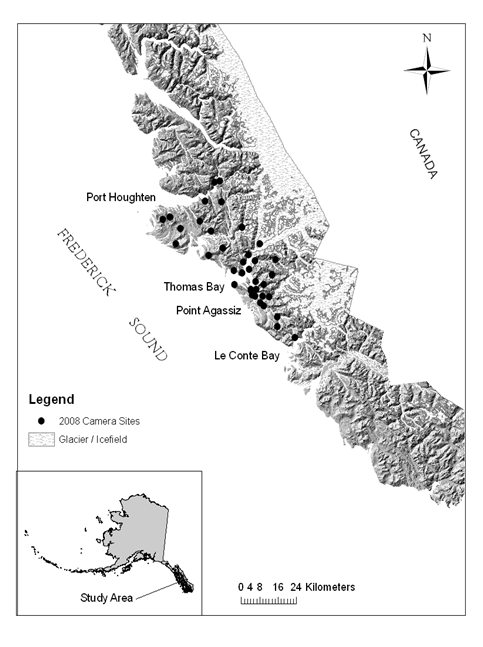
\includegraphics[height=3in]{Ch4/figs/wolverinelocs}
\end{center}
\caption{Wolverine camera trap locations from \citet{magoun_etal:2011}.
XXXXX this figure is way too small. Also, I would take out some of the
legends in the actual figure and put this into the figure legend
(e.g., what the dots mean and the grey area) XXXXXX
}
\label{scr0.fig.wolverinelocs}
\end{figure}

To carry-out an analysis of these data, we require the matrix of trap
coordinates and the encounter history data.  We store data in the
``scr flat format'' (see sec.  \ref{scr0.sec.formats} above), an
efficient file format which is easily manipulated and also used as the
input file format in {\bf SPACECAP} \citep{gopalaswamy_etal:2012} and
in the {\bf R} package \mbox{\tt SCRbayes} \citep{russell_etal:2012}.
To illustrate this format, the wolverine data are available in the
package \mbox{\tt scrbook} by typing:
\begin{verbatim}
data(wolverine)
\end{verbatim}
which contains a list having elements \mbox{\tt wcaps} and
\mbox{\tt wtraps}.
The ``encounter data file''
\mbox{\tt wcaps}  has 3 columns and 115 rows, each representing a
unique encounter event including the trap identity, the individual
identity and the sample occasion index (\mbox{\tt sample}).
The first 10 rows of this matrix are as
follows:
{\small
\begin{verbatim}
> wolverine$wcaps[1:10,]
       trapid individual sample
  [1,]      1          2    127
  [2,]      1          2    128
  [3,]      1          2    129
  [4,]      1         18    130
  [5,]      2          3    106
  [6,]      2         18    104
  [7,]      5          5     73
  [8,]      5          5     89
  [9,]      6         18    117
 [10,]      6         18    118
\end{verbatim}
}
Each row is a unique 
individual/trap encounter, and the 3 variables (columns) are: 
\mbox{\tt trapid} -- an
integer that runs from \mbox{\tt 1:ntraps}, \mbox{\tt individual} runs from
\mbox{\tt 1:nind} and
\mbox{\tt sample} 
runs from \mbox{\tt 1:nperiods}. Often (as the case here) \mbox{\tt
  sample} 
will
correspond to daily sample intervals. The variable \mbox{\tt trapid} will have to
correspond to the row of a matrix containing the trap coordinates - in
this case the file \mbox{\tt wtraps} which we describe further below.

Note that the information provided in this encounter data file
\mbox{\tt wcaps}
does not represent a completely informative summary
of the data. For example, if no individuals were captured in a certain
trap or during a certain period, then this compact data format will
have no record. Thus we will need to know \mbox{\tt ntraps} XXXX? in general, we have multiple definitions of these things and we need to be consistentXXXXXX and \mbox{\tt nperiods} when
reformatting this SCR data format into a 2-d encounter frequency
matrix or 3-d array. In addition, the encounter data file does not
provide information about which periods each trap was operated. This
additional information is also necessary as the trap-specific sample
sizes must be passed to {\bf BUGS} as data. We provide this information in a
2nd data file, along with the trap coordinates, in the 
 ``trap deployment'' file which is described
below.

For our purposes we
need to convert the \mbox{\tt wcaps} file
into the $n \times J$ array of
binomial encounter frequencies, although more general models might
require an encounter-history formulation of the model which requires a
full 3-d array.  To obtain our $n \times J$ encounter frequency
matrix, we do this the hard way by first converting the encounter data
file into a 3-d array and then summarize to trap totals. We have a
handy function \mbox{\tt SCR23darray.fn} which takes the compact
encounter data file with optional arguments  \mbox{\tt ntraps} and \mbox{\tt nperiods}, and
converts it to a 3-d array, and then we use the {\bf R} function
\mbox{\tt apply} to summarize over the ``sample'' period dimension (by
convention here, this is the 2nd dimension). To apply this to the
wolverine
data in order to compute the 3-d array we do this:
{\small
\begin{verbatim}
y3d <-SCR23darray.fn(wolverine$wcaps,wolverine$wtraps)
y <- apply(y3d,c(1,3),sum)
\end{verbatim}
}
See the help file for more information on \mbox{\tt SCR23darray.fn}.
The 3-d array is necessary to fit certain types
of models (e.g., behavioral response) and this is why we sometimes
will require this maximally informative 3-d data format but, here, we
analyze the summarized data.



The other important information needed to fit SCR models is the
``trap deployment'' file
which provides the additional information
not contained in the encounter data file. The traps file has \mbox{\tt
  nperiods} $+ 3$ columns. The first column is assumed to be a trap identifier,
columns 2 and 3 are the easting and northing coordinates (assumed to
be in a Euclidean coordinate system), and columns 4 to (\mbox{\tt nperiods} + 3)
are binary indicators of whether each trap was operational in each
time period. The first 10 rows (out of 37) and 10 columns (out of 167)
of the trap deployment file for the wolverine data are:
{\small
\begin{verbatim}
> wolverine$wtraps[1:10,1:10]

   Easting Northing 1 2 3 4 5 6 7 8 
1   632538  6316012 0 0 0 0 0 0 0 0
2   634822  6316568 1 1 1 1 1 1 1 1
3   638455  6309781 0 0 0 0 0 0 0 0
4   634649  6320016 0 0 0 0 0 0 0 0
5   637738  6313994 0 0 0 0 0 0 0 0
6   625278  6318386 0 0 0 0 0 0 0 0
7   631690  6325157 0 0 0 0 0 0 0 0
8   632631  6316609 0 0 0 0 0 0 0 0
9   631374  6331273 0 0 0 0 0 0 0 0
10  634068  6328575 0 0 0 0 0 0 0 0
\end{verbatim}
}
This tells us that trap 2 was operated in periods (days) 1-7 but the other
traps were not operational during those periods. It is extremely
important to recognize that each trap was operated for a variable
period of time and thus the binomial "sample size" is different for
each, and this needs to be accounted for in the {\bf BUGS} model specification.
To compute the vector of sample sizes $K$, and extract the trap
locations,  we do this:
\begin{verbatim}
traps<- wolverine$wtraps
traplocs<- traps[,1:2]
K<- apply(traps[,3:ncol(traps)],1,sum)
\end{verbatim}
This results in a matrix \mbox{\tt traplocs} which contains the coordinates of
each trap and a vector $K$ containing the number of days that each trap
was operational. We now have all the information required to fit a
basic SCR model in {\bf BUGS}.

Summarizing these data files for the wolverine study, we see that 21
unique individuals were captured a total of 115 times. Most
individuals were captured 1-6 times, with 4, 1, 4, 3, 1, and 2
individuals captured 1-6 times, respectively.  In addition, 1
individual was captured each 8 and 14 times and 2 individuals each
were captured 10 and 13 times.  The number of unique traps that
captured a particular individual ranged from 1-6, with 5, 10, 3, 1, 1,
and 1 individual captured in each of 1-6 traps, respectively, for a
total of 50 unique wolverine-trap encounters.  These numbers might be
hard to get your mind around whereas some tabular summary is often
more convenient. For that it seems natural to tabulate individuals by
trap and total encounter frequencies. The spatial information in SCR
data is based on multi-trap captures\footnote{I will add more 
context here on revision about spatial recaptures, lost recaptures,
ordinary recaptures. Function \mbox{\tt SCRsmy} in \mbox{\tt
  scrbook}}, 
and so, it is informative to
understand how many unique traps each individual is captured in. At
the same time, it is useful to understand how many total captures we have
of each individual because this is, in an intuitive sense, the
effective sample size.  So, we reproduce Table 1 from
\citet{royle_etal:2011jwm} which shows the trap and total encounter
frequencies:

\begin{table} [htp]
  \caption{Individual frequencies of capture for wolverines captured
    in camera traps in Southeast Alaska in 2008. Rows index unique
    trap frequenciesxxxxx $traps or trap frequencies ???$ xxxxxand columns represent total number of captures
    (e.g., we captured 4 individuals 1 time, necessarily in only 1
    trap; we captured 3 individuals 3 times but in 2 different traps).
%% This differs by 1 from Royle et al. 2011 table.
}
\centering
\begin{tabular}{c c c c c c c c c c c}
\hline
 & & & & & & & &  No.&of&captures \\
\hline
No. of traps & 1 & 2 & 3 & 4 & 5 & 6 & 8 & 10 &13 &14 \\
\hline
1 & 4 & 1 & 0 & 0 & 0 & 0 & 0 & 0 & 0 & 0 \\
2 & 0 & 0 & 3 & 2 & 0 & 2 & 1 & 2 & 0 & 0 \\
3 & 0 & 0 & 1 & 1 & 0 & 0 & 0 & 0 & 0 & 1 \\
4 & 0 & 0 & 0 & 0 & 0 & 0 & 0 & 0 & 1 & 0 \\
5 & 0 & 0 & 0 & 0 & 1 & 0 & 0 & 0 & 0 & 0 \\
6 & 0 & 0 & 0 & 0 & 0 & 0 & 0 & 0 & 1 & 0 \\
\hline
\end{tabular}
\end{table}


\subsection{Fitting the model in WinBUGS}

For illustrative purposes here we fit the simplest SCR model with the
half-normal distance function although we revisit these data with more
complex models in later chapters. The model is summarized by the
following 3 components:
\begin{itemize}
\item[(1)] $y_{ij}|{\bf s}_{i} \sim \mbox{Bin}(K, z_{i}\; p_{ij})$
\item[(2)] $p_{ij} = p_{0} \exp(-\alpha1 \; ||{\bf s}_{i}-x_{j}||^2)$
\item[(3)] $ {\bf s}_{i} \sim \mbox{Unif}({\cal S})$
\item[(4)] $ z_{i} \sim \mbox{Bern}(\psi)$
\end{itemize}
We assume customary flat priors on the structural (hyper-) parameters
of the model, $\alpha_{0} = \mbox{logit}(p_{0})$, $\alpha1$ and $\psi$.  It remains to define the
state-space ${\cal S}$. For this, we nested the trap array (Fig.
\ref{scr0.fig.wolverinelocs}) in a
 rectangular state-space extending $20$ km beyond the traps in each cardinal
direction.  We also considered larger state-spaces up to 50 km to
evaluate that choice.  The buffer of the state space should be large
enough so that individuals beyond the state-space boundary are not
likely to be encountered. Thus some knowledge of typical space usage
patterns of the species is useful.  For the analysis, 
we scaled the coordinate system 
so that a unit distance was equal to $10$ km, producing a rectangular
state-space of dimension $9.88 \times 10.5$ units ($area = 10374$ km$^2$)
within which the trap array was nested. As a general rule, we
recommend scaling the state-space so that it is defined near the
origin $(x,y)=(0,0)$. While the scaling of the coordinate system is
theoretically irrelevant, a poorly scaled coordinate system can
produce Markov chains that mix poorly.  For the scaled coordinate
system we fit models for various choices of a rectangular state-space
based on 
buffers from 1.0 to 5.0 units on the scaled coordinate system (10 km to
50 km). In the {\bf R} package \mbox{\tt scrbook} we provide a
function
\mbox{\tt wolvSCR0.fn} which will fit the basic SCR model. For
example, to fit the model in 
{\bf WinBUGS} using data augmentation with $M=300$ potential individuals,
using 3 Markov chains each of 12000 total iterations, discarding the
first 2000 as burn-in, we execute the following {\bf R} commands:
{\small
\begin{verbatim}
library("scrbook")
data(wolverine)
traps<-wolverine$wtraps
y3d <-SCR23darray.fn(wolverine$wcaps,wolverine$wtraps)
toad<-wolvSCR0.fn(y3d,traps,nb=12000,ni=2000,delta=1,M=300)
\end{verbatim}
}
The argument \mbox{\tt delta} determines the buffer size of the state-space.
Note that this analysis takes 
between 1-2 hours on many machines so we recommend trying it out with
lower values of $M$ and fewer iterations.
The output
follows (note, we have a parameter ``sigma'' which we discuss
shortly)\footnote{Final as of 1/11/2012. 
output saved in \mbox{\tt wolv-buffer-study.txt}}:

{\small
\begin{verbatim}
All based on 3 chains, 12k iters, 2k burn, 30k total
Buffer = 10 km
           mean    sd   2.5%    25%    50%    75%  97.5% Rhat n.eff
psi        0.13  0.03   0.08   0.11   0.13   0.15   0.20    1 10000
sigma      0.65  0.06   0.55   0.61   0.64   0.68   0.76    1  1800
p0         0.06  0.01   0.04   0.05   0.06   0.06   0.08    1 20000
N         39.63  6.70  29.00  35.00  39.00  44.00  54.00    1  7100
D          5.92  1.00   4.33   5.22   5.82   6.57   8.06    1  7100
beta       1.23  0.21   0.85   1.08   1.22   1.36   1.66    1  1800
deviance 410.05 12.06 388.70 401.50 409.20 417.80 435.60    1 22000

Buffer = 15 km
 n.sims = 30000 iterations saved
           mean    sd   2.5%    25%    50%    75%  97.5% Rhat n.eff
psi        0.16  0.04   0.10   0.14   0.16   0.19   0.25    1  3800
sigma      0.64  0.06   0.54   0.60   0.64   0.67   0.76    1   510
p0         0.06  0.01   0.04   0.05   0.06   0.06   0.08    1 17000
N         48.77  9.19  34.00  42.00  48.00  54.00  69.00    1  3300
D          5.78  1.09   4.03   4.98   5.69   6.40   8.18    1  3300
beta       1.25  0.21   0.86   1.10   1.24   1.39   1.70    1   510
deviance 411.00 12.16 389.50 402.40 410.30 418.70 437.00    1  5400

Buffer = 20 km
           mean    sd   2.5%    25%    50%    75%  97.5% Rhat n.eff
psi        0.20  0.05   0.12   0.17   0.20   0.23   0.30    1 16000
sigma      0.64  0.06   0.54   0.60   0.63   0.67   0.76    1  1200
p0         0.06  0.01   0.04   0.05   0.06   0.06   0.08    1  1900
N         59.84 11.89  40.00  51.00  59.00  67.00  86.00    1 20000
D          5.77  1.15   3.86   4.92   5.69   6.46   8.29    1 20000
beta       1.26  0.21   0.87   1.11   1.25   1.40   1.71    1  1200
deviance 411.01 12.36 389.10 402.30 410.20 418.80 437.50    1  1500

Buffer = 25 km
           mean    sd   2.5%    25%    50%    75%  97.5% Rhat n.eff
psi        0.24  0.05   0.15   0.20   0.24   0.28   0.36    1  3400
sigma      0.64  0.05   0.54   0.60   0.63   0.67   0.75    1  3600
p0         0.06  0.01   0.04   0.05   0.06   0.06   0.08    1  5000
N         72.40 14.72  47.00  62.00  71.00  81.00 105.00    1  2700
D          5.79  1.18   3.76   4.96   5.67   6.47   8.39    1  2700
beta       1.26  0.21   0.88   1.12   1.25   1.40   1.71    1  3600
deviance 411.35 12.23 389.70 402.70 410.55 419.20 437.20    1 30000

Buffer = 30 km
           mean    sd   2.5%    25%    50%    75%  97.5% Rhat n.eff
psi        0.29  0.06   0.18   0.24   0.28   0.33   0.43    1  3100
sigma      0.63  0.05   0.54   0.60   0.63   0.67   0.75    1  5600
p0         0.06  0.01   0.04   0.05   0.06   0.06   0.08    1 11000
N         86.42 17.98  56.00  74.00  85.00  97.00 126.02    1  3900
D          5.82  1.21   3.77   4.98   5.72   6.53   8.49    1  3900
beta       1.27  0.21   0.88   1.12   1.26   1.41   1.71    1  5600
deviance 411.06 12.37 389.20 402.50 410.20 418.90 437.60    1 10000

Buffer = 35 km
           mean    sd   2.5%    25%    50%    75%  97.5% Rhat n.eff
psi        0.34  0.08   0.21   0.29   0.34   0.39   0.50    1 30000
sigma      0.63  0.05   0.54   0.60   0.63   0.67   0.75    1  4500
p0         0.06  0.01   0.04   0.05   0.06   0.06   0.08    1 24000
N        101.79 21.54  65.00  87.00 100.00 115.00 148.00    1 30000
D          5.85  1.24   3.74   5.00   5.75   6.61   8.51    1 30000
beta       1.27  0.21   0.89   1.12   1.25   1.40   1.70    1  4500
deviance 411.10 12.20 389.50 402.40 410.30 418.90 437.20    1 22000

Buffer = 40 km
           mean    sd   2.5%    25%    50%    75%  97.5% Rhat n.eff
psi        0.39  0.09   0.24   0.33   0.39   0.45   0.60 1.01   480
sigma      0.64  0.05   0.54   0.60   0.63   0.67   0.75 1.01   410
p0         0.06  0.01   0.04   0.05   0.06   0.06   0.08 1.00 21000
N        118.05 26.14  75.00 100.00 116.00 133.00 178.00 1.01   450
D          5.87  1.30   3.73   4.97   5.76   6.61   8.84 1.01   450
beta       1.27  0.21   0.89   1.12   1.25   1.40   1.72 1.01   410
deviance 411.37 12.35 389.30 402.60 410.60 419.30 437.50 1.00  9700

Buffer = 45 km
           mean    sd   2.5%    25%    50%    75%  97.5% Rhat n.eff
psi        0.45  0.10   0.28   0.38   0.44   0.51   0.66    1  3600
sigma      0.64  0.05   0.54   0.60   0.63   0.67   0.75    1 10000
p0         0.06  0.01   0.04   0.05   0.06   0.06   0.08    1  8100
N        134.43 28.68  85.00 114.00 132.00 153.00 196.00    1  3300
D          5.83  1.24   3.68   4.94   5.72   6.63   8.50    1  3300
beta       1.26  0.21   0.88   1.11   1.24   1.39   1.69    1 10000
deviance 411.36 12.19 389.60 402.70 410.60 419.10 437.30    1  9400

Buffer = 50 km
           mean    sd   2.5%    25%    50%    75%  97.5% Rhat n.eff
psi        0.51  0.11   0.31   0.43   0.50   0.57   0.74    1  3200
sigma      0.63  0.05   0.54   0.60   0.63   0.67   0.75    1  4700
p0         0.06  0.01   0.04   0.05   0.06   0.06   0.08    1  3300
N        151.61 31.65  96.00 129.00 149.00 172.00 221.00    1  3400
D          5.79  1.21   3.66   4.92   5.69   6.56   8.43    1  3400
beta       1.27  0.21   0.89   1.12   1.25   1.40   1.70    1  4700
deviance 410.81 12.18 389.20 402.30 410.10 418.50 436.70    1 30000

Buffer = 55 km 
           mean    sd   2.5%    25%    50%    75%  97.5% Rhat n.eff
psi        0.56  0.12   0.35   0.48   0.55   0.64   0.82 1.01   260
sigma      0.64  0.05   0.54   0.60   0.63   0.67   0.76 1.00  1600
p0         0.06  0.01   0.04   0.05   0.06   0.06   0.08 1.00 30000
N        169.28 35.81 108.00 143.00 166.00 192.00 247.00 1.01   260
D          5.73  1.21   3.66   4.84   5.62   6.50   8.36 1.01   260
beta       1.25  0.21   0.88   1.11   1.24   1.39   1.69 1.00  1600
deviance 411.28 12.38 389.40 402.60 410.50 419.10 437.50 1.00 26000
\end{verbatim}
}

We see that the estimated density is roughly consistent as we increase
the state-space buffer from $15$ to $50$ $km$. We do note that the data
augmentation parameter $\psi$ (and, correspondingly, $N$) increase with
the size of the state space in accordance with the deterministic
relationship $N= D*A$. However, density is more or less constant as we
increase the size of the state-space beyond a certain point.  For the
10 $km$ state-space buffer, we see a slight effect on the posterior
distribution of $D$. This is not a bug but rather a feature. As we noted
above, the state-space is part of the model.


\subsection{Thoughts on the Wolverine Analysis}

Our point estimate of wolverine density from this study, using the
posterior mean from the state-space based on the 20
$km$ buffer, is 
approximately $5.77$ individuals/1000 $km^2$ with  a 95\% posterior
interval of $[3.86, 8.29]$. Density is estimated imprecisely
which might not be surprising given the low sample size ($n=21$
individuals!). This seems to be a basic feature of carnivore studies
although it should not (in our view) preclude the study of their
populations nor attempts to estimate density or vital rates.

One thing we haven't talked about yet is that we can calibrate the
desired size of the state-space by looking at the estimated home range
radius of the species. For some models it is possible to convert the
parameter $\alpha1$ directly into the home range radius (sec. 
XXX MISSING XYZ). For the half-normal model we interpret the half-normal scale
parameter $\sigma$, which is related to $\alpha1$ by $\alpha1 =
1/(2\sigma^2)$, as the radius of a bivariate normal movement model. 
In this case $\sigma = 1.82$ standardized units, which corresponds to 18.2 $km$ and translates into a home range area of XXXX MISSING XXXXX. 

It is worth thinking about this model, and these estimates, computed
under a rectangular state space roughly centered over the trapping
array (Fig. \ref{scr0.fig.wolverinelocs}).
Does it make sense to define the state-space to
include, for example, ocean? What are the possible consequences of
this? What can we do about it?  There's no reason at all that the
state space has to be a regular polygon -- we defined it as such here
strictly for convenience and for ease of implementation in {\bf WinBUGS}
where it enables us to specify the prior for the activity centers as
uniform priors for each coordinate.  While it would be possible to
define a more realistic state-space using some general polygon GIS coverage, it
might take some effort to implement that in the {\bf BUGS} language
but it is not difficult to devise custom MCMC algorithms to do that
(see Chapt. \ref{chapt.mcmc}).
Alternatively, we recommend
using a discrete representation of the state-space -- i.e., approximate
${\cal S}$ by a grid of $G$ points. We discuss this in sec. 
\ref{scr0.sec.discrete}.

\section{The Implied Model of Space Usage:
Implied resource selection model? 
Implied home range model?
}
\label{sec.scr0.implied}

We have implied a few times that the model for detection probability
is somehow related to animal ``home range'' somehow. Here 
we explore the nature of that relationship.  While we have used the
term ``home range'' and other jargon (territory, activity center,
etc..) almost interchangeably, what we really mean to imply is
something that would be more more clearly identified as ``space
usage'' which we view in a manner equivalent to what is normally
called resource selection. If the resource is only space, i.e., with
no explicit covariates, then space usage is a more descriptive term
but, otherwise (Chapt. XXXX) we take the term as being analogous to
 ``resource selection''.

We believe that thinking about detection models as models of
space usage of animals is more sensible and interpretable in the manner
that we describe here.  A given detection model will imply a a model
of space usage -- amount and extent of area used some prescribed
percentage of the time -- i.e., 95\% of animal movements are within
some distance from an individual's activity center. 
In that sense, i.e., if we equate that area to ``home
range'', then the detection model implies a model of home range. In
other words, there is an implicit home range model underlying a given
detection probability model. 

i.e., ``how much space encompases 95\% of the movement outcomes of an
individual -- or the space used.''

Intuitively, the detection function of SCR models is related to home
range area or space usage of individuals.  This is because we
interpret the detection model as the composite of two processes -
movement about the home range i.e., space usage, and detection {\it conditional on use} (see
chapter 1.XYZ). Formally we decompose encounter probability according
to (all things conditional on ${\bf s}$ here):
\[
 \Pr(encounter at x|s) = \Pr(encounter | usage of x, s) \Pr(usage of x|s).
\]


How do we chararacterize $Pr(usage)$?  First of all we note that it is
not a proability distribution on $x$ like a classical RSF. Instead,
think of an animal using space for some period of time and accuulating
a history of space usage (being a bunch of values of $x$) and we
random sample a single value. Define $\pi(x|s)$ to be a probability
distribution of that value, i.e., $\pi(x|s)$ {\it is} a probability
distribution of $x$. following standard notions of this stuff we
use this function here:
\[
\pi(x|s) =  \frac{ exp(  -d(s,x)^{2}/(2\sigma^{2})) }
{ \sum_{x} exp(  -d(s,x)^{2}/(2\sigma^{2})) }
\]
therefore clearly the space used by an individual will be proportional
to whatever kernel we stick in for the numerator. The customary
choice, in RSF literature, is to use the negative exponential function
but here we have the Gaussian kernel because we like that.

This is a pdf of $x$ and in sampling a populationi of individuals
using traps or other devices we set them out and they accumulate
potential detections over a period of time. Thus whether or not a
point $x$ is {\it used} (at all) depends on some unknown rate of use
by the individual over whatever period of time the devices are
active. This is something we can't hope to estimate or model in most
cases but we imagine that over a period of time usage is characterized
by a rate of usage $\lambda_{0}$ so that amount of usage of $x$ is
\[
m(x,s) = Poisson(\lambda_{0} \pi(x|s) ) 
\]
which isn't really an important assumption because note that by
conditioning on the total again it retains the (natural) multionomial
distribution. So we ask ``if a guy uses space 100 times, where is that
space being used?'' and the histogram of usage is proportional to
$\pi(x|s)$. But over time timee intrval we expect this amount to be
random and then whether we detect a guy or not at $x$ occurs if
$m(x|s)>0$. That is
\[
Pr(y=1) = 1-exp(-\lambda_{0} \pi(x|s))
\]
Some call this a ``hazard model.''  This is why we like the cloglog
link function in XXXXX (royle et al. 2009ecol).
So this all comes about by introducing a latent process of ``usage''
accumulating over time.    
We could just as well say $Pr(y=1) \propto \pi(x|s)$ which is the
half-normal model. 


Ok back to this thing: 
\[
 \Pr(encounter at x|s) = Pr(encounter | usge of x,s) Pr(usage of x|s).
\]
Therefore, if we imagine that encounter probability was perfect,
everywhere, and animals moved around according to some bivariate
distribution $\Pr(movement to x | s) = g(x,s)$ then a sensible summary
of home range (or space usage) is the area that contains 95\% of the
mass of $g(x,s)$. i.e., 95\% of all animal locations.  In SCR models it
is not always so clear how to compute this because (1) most detection
functions do not correspond to a specific bivariate movement
distribution g(x,s) and (2) we only get to observe ``movement outcomes''
where we happen to have traps, and even then we don't observe those
perfectly (just when the movement outcome is near a trap).


\subsection{Bivariate normal case}  

There is (at least) one detection model that allows a direct
conversion to a home range model based on space usage. This is the
model that arises under a bivariate normal movement model.  In fact there are two representations for this detection model. The obvious one is:
\[
p(x,s) = \lambda_{0} \exp(-\theta*||{\bf x}-{\bf s}||^2)         
\]
Thinking about this under our decomposition mentioned above, i.e., 
\[
Pr(detection at x | s) = Pr(detection | x used)Pr(x used | s)
\]
It seems reasonable to imagine that the conditional probability of
detection is constant or at least not dependent on ${\bf s}$ (but it
might depend on ${\bf x}$, the trap location, and that would be ok,
see chapt. XXXXX) and we therefore recognize the 2nd part is the
kernel of a bivariate probability distribution which is an explicit
movement model that is widely used.  For the bivariate normal case
then:
\[
\Pr(detection at x | s) = lam0*const*exp(- (1/(2*sigma*sigma))*dist(x,s)^2)
		            =  p0*exp(- (1/(2*sigma*sigma))*dist(x,s)^2)
\]
Here ``const'' is the part of the bivariate normal density that allows
it to integrate to 1. Therefore the effective local encounter rate is
the product of the conditional probability of detection lam0 and this
normalizing constant.

Under this model we can compute precisely the effectively home range
area. In particular, imagining that movement outcomes are bivariate
normal then $||{\bf x}-{\bf s}||^2$ has a chi-square distribution with
2 d.f. and so we need to find the constant $B(\alpha)$ such that
$\Pr(d\le B(\alpha)) = 1-\alpha$, i.e, the constant $B(\alpha)$ that
encloses 95\% of all realized distances. The constant $B(\alpha) =
\sigma*\sqrt{q(2,\alpha)}$. For $\alpha=.05$, $q(2,\alpha) = 5.99$ so
as an example for $\sigma=1$, $B(\alpha) = 1*\sqrt{5.99} = 2.447$ and
therefore 95\% of the movement outcomes will be within 2.447 units of
the home range center. So the basic idea is that we can estimate
``sigma'' by fitting the detection model above (either form) and
plugging it into this expression for $B(\alpha)$ to obtain the home
range radius that contains 95\% of movement outcomes.

\subsection{Hazard formulation}

An alternative bivariate normal model is based on a bivariate normal hazard rate:
\[
p(x,s) = 1-exp(-lam0*exp(-beta*||x-s||^2))
\]
It is perhaps not immediately clear why or even whether these should
produce the same home range area for a given beta, but it turns out
they do!  Its not obvious to me why, so a little bit of analysis is in
order for sure.

\subsection{Empirical analysis}

For many detection models we can compute the 95\% area empirically
by taking a fine grid of points and 
either simulating movement outcomes with probabilities proportional to
$p(x,s)$ and accumulating area around ${\bf s}$ or else we can do this precisely
by finding the distance $||x-s||$ within which 95\% of all movements are
concentrated. 

Under any detection model, movement outcomes will occur
in proportion to $p(x,s)$ and so we can define probabilities according
to:
\[
 \pi(x|s) =\frac{p(x,s)}{\sum_{x} p(x,s) }
\]
i.e., under the 2-part decomposition noted above, the use 
distribution has to have probabilities $\pi({\bf x}|{\bf s})$. In
other words, $\pi({\bf x}|{\bf s})$ is a discrete representation of
this movement distribution.  Given the probabilities $\pi({\bf
  x},{\bf s})$ for all ${\bf x}$ we can find the value of ${\bf x}_{0}$ such that
$\sum_{{\bf x}_0 s.t. ||x0-s||} \pi({\bf x},{\bf s}) \le 0.95$.
Here is an algorithm for doing that (below). But first we simulate some data.

{\small
\begin{verbatim}
# source SCR utility functions
source("utilities.R")

# individual centered at (3,3) with 10000 "potential trap" locations
s<-c(3,3)
x1<- rep(seq(0,6,,100),100)
x2<- sort(rep(seq(0,6,,100),100))
delta<- min(diff(x1[1:10]))
area<- ( (6+delta/2)^2)/10000

# plot those trap locations
X<-cbind(x1,x2)
plot(X,pch=".")

# compute distances and encounter probabilities under some model
D<-sqrt(  ( s[1]-x1)^2  + (s[2]-x2)^2)
sigma<- .396
lp<-  -2.72 -(1/(2*sigma*sigma))*D*D
p<- 1-exp(-exp(lp))
# 2 alternative link functions
#p<-  exp(lp)
#p<- expit(lp)

# plot this surface
spatial.plot(X,p)

# use these probabilities to simulate movement outcomes
pi.probs <- p/sum(p)
\end{verbatim}
}

Next we find the value of ${\bf x}_0$ such that $\sum_{x<=x0}
\pi({\bf x}|{\bf s}) = 0.95$. We do this by starting at some small
value of ${\bf x}_0$ and then summing the appropriate values of
$\pi$. If the total is $< 0.95$ then we increase ${\bf x}_0$ by a
little bit (1\% below), otherwise if the total area $\ge 0.95$ then we
break out of the loop. Here a crude root-finding algorithm:

\begin{verbatim}
# find area that contains 95% of movements
x0<-.2
repeat{
in.hr<- D<=x0
total<- sum(pi.probs[in.hr])  
cat("Total area: ",total,fill=TRUE)
if(total>=.95) {
print(x0)    # if condition is met, break
break
}
x0<-x0*1.01  # otherwise increase x0
}
\end{verbatim}

If we execute this root-finding code for the simulated data above we
have the following, where the number output is the desired ${\bf x}_0$:
\begin{verbatim}
Total area:  0.9484948
Total area:  0.9500548
[1] 0.973035
\end{verbatim}

What this means is that ${\bf x}_0 = 0.973$ is the radius that
encloses about 95\% of all movements under the model above. Therefore
the area is about $\pi*.973*.973 = 2.97 \approx 3.0$.
You can change the intercept of the model and find that it has no affect. I don't know if that works out across all classes of models or not. Note that the intercept never affects $p$ multiplicatively and so its not obvious (to me) that it shouldn't have an affect (except somewhat intuitively perhaps).

The point of doing this is that we can now apply this process of simulating data to find the 95\% home range area for any detection model with prescribed parameter values.  Similarly, we can also work backwards. That is: For any desired 95\% home range area, we can find the coefficient on distance that produces that home range area (assuming intercept to have no affect). Here is a function for doing that:

First, define an objective function to find the root of. This is a
function of $\sigma$ and also the target home range area (``target'')
which is fixed:
\begin{verbatim}
obj<-function(sigma,target= 3 ){
a<-1/(2*sigma*sigma)
lp<- -2 -a*D*D
p<- 1-exp(-exp(lp))

pi.probs<- p/sum(p)
x0<-.1
repeat{
in.hr<- D<=k
total<- sum(pi.probs[in.hr])  
#cat("Total area: ",total,fill=TRUE)
if(total>=.95) {
print(x0)
break
}
x0<-x0*1.01
}
hr.area<- pi*x0*x0
print(hr.area)
ss<-  (hr.area - target)^2
ss
}
\end{verbatim}


Now we use the {\bf R} function optimize to locate the optimal value
of $\sigma$ - optimal here being the value of $\sigma$  that makes
home range area minus ``target''  equal to 0:
\begin{verbatim}
tmp<-optimize(obj,interval=c(.1,5),target=3)
sigma.best<- tmp$minimum

> sigma.best
[1] 0.3957799
\end{verbatim}

We see this is equal to 0.396 which is the value we simulated data from above - so things seem to be working in an orderly manner. 

\subsection{Why do we care about this stuff?}

One important reason that we need to be able to deduce ``home range
area'' from a detection model is so that we can compare different
models on the same biological footing. 
As we noted somewhere else (XXXX in ch 4) the scale parameter $\sigma$
relateds to 95\% area in a different manner under each detection
function and so we want to be able to convert different models to the
same currency. 


RSF/telemetry data: In chapter XXXX 
we consider the case in which a sample of individuals produces encounter history data suitable for SCR models and, in addition, we have telemetry relocations on a subset of individuals - within the same population or not, it probably doesn't matter.  We assume the telemetry fixes are made sufficiently far apart so that the locations represent independent movement outcomes of individuals within their home range [note: otherwise we need to devise a model for correlated outcomes which is difficult, except in the bivariate normal situation].

Conceptually we regard these two data sets as independent. Let $y[i]$
denote the individual encounter history data for individual i and let
$u[m,t=1,\ldots,T]$ denote the telemetry locations for individual m. If
we have a common model in terms of space usage then we can combine the
two data sources to improve information.  Bivariate normal model is
covered in chapter XXXX but we can also, I think, handle the general
case: Some other detection probability models probably do correspond
to specific bivariate distributions that can be evaluated and
simulated from directly. In general, we can view the telemetry
outcomes u[i,t] as realizations of a point process with intensity
function
\[
\pi(x,s) = p(x,s)/[ \int_{x} p(x,s) ]
\]
Which allows us to analyze models with auxiliary data by MCMC or directly by likelihood.



Modeling space usage. We imagine that each pixel $x$ has a covariate
associated with it and the probability of an individual going there
should be a function of that covariate..... this is different than
Richard's chapter 14 stuff because we are thinking here of modeling
variation {\it within} a home-range. 


\section{Constructing Density Maps}
\label{scr0.sec.mapping}

One of the most useful aspects of SCR models is that they are
parameterized in terms of individual locations - i.e., {\it where}
each individual lives -- and, thus, we can compute many useful or
interesting summaries of the activity centers.  For example, we can
make a spatial density plot by tallying up the number of activity
centers ${\bf s}_{i}$ in pixels  of arbitrary size and then producing a
nice multi-color spatial plot of those which, we find, increases the
acceptance probability of your manuscripts by a substantial amount.
We discussed in Chapt. \ref{chapt.glms} the idea of estimating derived
parameters from MCMC output. In SCR models, there are many derived
parameters that are functions of the latent point locations $({\bf
  s}_{1},\ldots, {\bf s}_{N})$. In the present context, the number of
individuals living in any well-defined polygon is a derived
parameter. Specifically, let $B({\bf x})$ indicate a pixel centered at
${\bf x}$ then
\[
N({\bf x})=\sum_{i} I({\bf s}_{i} \in B({\bf x}))
\]
XXXXXX say that I() is the indicator function XXXX

is the population size of pixel XXX change box to pixel XXXXX $B({\bf x})$, and $D({\bf x}) = N({\bf
  x})/||B({\bf x})||$ is the local density. These are just ``derived
parameters'' (see Chapt.  \ref{chapt.glms}) which are estimated from
MCMC output using the appropriate Monte Carlo average. One thing to be
careful about, in the context of models in which $N$ is unknown, is
that, for each MCMC iteration $m$, we only tabulate those activity
centers which correspond to individuals in the sampled
population, i.e., for which the data augmentation variable $z_{i} =
1$.  In this case, we take all of the output for MCMC iterations
$m=1,2,\ldots,\mbox{\tt niter}$ and compute this summary:
\[
   N({\bf x},m) = \sum_{z_{i,m}=1} I(s_{i,m} \in B({\bf x}))
\]
Thus, $N({\bf x},1),N({\bf x},2),\dots,$ is the Markov chain for
parameter $N({\bf x})$.  In what follows we will provide a set of {\bf
  R} commands for doing this calculation and making a basic image
plot from the MCMC output.

{\flushleft \bf Step 1:} Define the center points of each box, $B({\bf
  x})$, or point at which local density will be estimated:
\begin{verbatim}
xg<-seq(Xl,Xu,,50)
yg<-seq(Yl,Yu,,50)
\end{verbatim}

{\flushleft \bf Step 2:} Extract the MCMC histories for the activity
centers and the data augmentation variables.  Note that these are each
$N \times \mbox{\tt niter}$ matrices:
\begin{verbatim}
Sxout<-out$sims.list$s[,,1]
Syout<-out$sims.list$s[,,2]
z<-out$sims.list$z
\end{verbatim}

{\flushleft \bf Step 3:} We associate each coordinate with the proper
box using the {\bf R} command \mbox{\tt cut()}. Note that we keep only
the activity centers for which $z=1$ (i.e., individuals that belong to
the population of size $N$):
\begin{verbatim}
Sxout<-cut(Sxout[z==1],breaks=xg,include.lowest=TRUE)
Syout<-cut(Syout[z==1],breaks=yg,include.lowest=TRUE)
\end{verbatim}

{\flushleft \bf Step 4:} Use the \mbox{\tt table()} command to tally
up how many activity centers are in each $B(x)$:
\begin{verbatim}

Dn<-table(Sxout,Syout)
\end{verbatim}

{\flushleft \bf Step 5:} Use the \mbox{\tt image()} command to display
the resulting matrix.
\begin{verbatim}
image(xg,yg,Dn/nrow(z),col=terrain.colors(10))
\end{verbatim}
Praise the Lord! This map is somewhat useful or at least it looks
pretty and will facilitate the publication of your papers.

It is worth emphasizing here that density maps will not usually appear
uniform despite that we have assumed that activity centers are
uniformly distributed. This is because the observed encounters of
individuals provide direct information about the location of the
$i=1,2,\ldots,n$ activity centers and thus their ``estimated''
locations will be affected by the observations. In a limiting sense,
were we to sample space intensely enough, every individual would be
captured a number of times and we would have considerable information
about all $N$ point locations. Consequently, the uniform prior would
have almost no influence at all on the estimated density surface in
this limiting situation. Thus, in practice, the influence of the
uniformity assumption decreases as the fraction of the population
encountered increases.

{\bf On the non-intuitiveness of \mbox{\tt image()} } -- the {\bf R}
function \mbox{\tt image()}, invoked for a matrix $M$ by \mbox{\tt image(M)}, might
not be very intuitive to some -- it plots $M[1,1]$ in the lower left
corner. If you want $M[]$ to be plotted ``as
you look at it'' then $M[1,1]$ should be in the upper left corner.  We
have a function \mbox{\tt rot()} which does that. If you do \mbox{\tt image(rot(M))} then it
puts it on the monitor as if it was a map you were looking at.  You
can always specify the $x$ and $y-$ labels explicitly as we did above.

{\bf Spatial dot plots } -- Now here is a cruder version based on the
``spatial dot map'' function \mbox{\tt spatial.plot}, which uses
the function \mbox{\tt image.scale()}.
The \mbox{\tt spatial.plot} function requires arguments of point
locations and the resulting value to be displayed:
\begin{verbatim}
spatial.plot<- function(x,y){
 nc<-as.numeric(cut(y,20))
 plot(x,pch=" ")
 points(x,pch=20,col=topo.colors(20)[nc],cex=2)
 image.scale(y,col=topo.colors(20))
}
# To execute the function do this:
spatial.plot(cbind(xg,yg), Dn/nrow(z))
\end{verbatim}

\subsection{Example: Wolverine density map. }
xxxxx$At places like this, where you revisit an earlier example, I would spend 1-2 sentences to remind the reader of what this is about. E.g., say that this is in SE Alaska in 2007 $xxxxxx
The {\bf R} commands for producing density maps from MCMC output of
spatial capture-recapture models is provided in the {\bf R} function
\mbox{\tt SCRdensity} in the package \mbox{\tt scrbook}. 
We used the posterior output from the wolverine model fitted previously
to compute a relatively coarse version of a density map, using a $10 \times
10$ grid (Fig. \ref{scr0.fig.density10x10}) and using a $30 \times 30$
grid (Fig. \ref{scr0.fig.density20x20}) for a fine-scale map. The {\bf R} commands for
producing such a plot (for short MCMC run) are as follows:
{\small
\begin{verbatim}
library("scrbook")
data(wolverine)
traps<-wolverine$wtraps
y3d <-SCR23darray.fn(wolverine$wcaps,wolverine$wtraps)
# this takes 341 seconds on a standard CPU circa 2011
unix.time(bln<-wolvSCR0.fn(y3d,traps,nb=1000,ni=2000,delta=1,M=100))
Sx<-bln$sims.list$s[,,1]
Sy<-bln$sims.list$s[,,2]
w<- bln$sims.list$w
obj<-list(Sx=Sx,Sy=Sy,w=w)
tmp<-SCRdensity(obj,scalein=100,scaleout=100)
\end{verbatim}
In these figures density is
expressed in units of individuals per $100$ $km^2$, while the area of
the pixels is about 103.7 $km^2$ and 11.5 $km^2$, respectively. That
calculation is based on:
\begin{verbatim}
> total.area<- (Yu-Yl)*(Xu-Xl)*100
> total.area/(10*10)
[1] 103.7427
> total.area/(30*30)
[1] 11.52697
\end{verbatim}

A couple of things are worth noting: First is that as we move away
from ``where the data live'' - away from the trap array - we see that
the density approaches the mean density. This is a property of the
estimator as long as the ``detection function'' decreases sufficiently
rapidly as a function of distance.
Relatedly, it is also a property of statistical smoothers
such as splines, kernel smoothers, and regression smoothers -
predictions tend toward the global mean as the influence of data
diminishes. Another way to think of it is that it is a consequence of
the prior - which imposes uniformity, and as you get far away from the
data, the predictions tend to the prior. xxxxx$is this correct ? I would have thought, they tend to the mean of what the prior AND the data say it should be ?$ xxxxx The other thing to note about
this map is that density is not $0$ over water (although the coastline
is not shown). This might be perplexing
to some who are fairly certain that wolverines do not like
water. However, there is nothing about the model that recognizes water
from non-water and so the model predicts over water {\it as if} it
were habitat similar to that within which the array is nested. But,
all of this is ok as far as estimating density goes and, furthermore,
we can compute valid estimates of $N$ over any well-defined region which
presumably wouldn't include water if we so wished. xxxx$xperhaps might simply say that pixels covered mostly by water could be masked in the plot ?$xxxx

\begin{figure}
\begin{center}
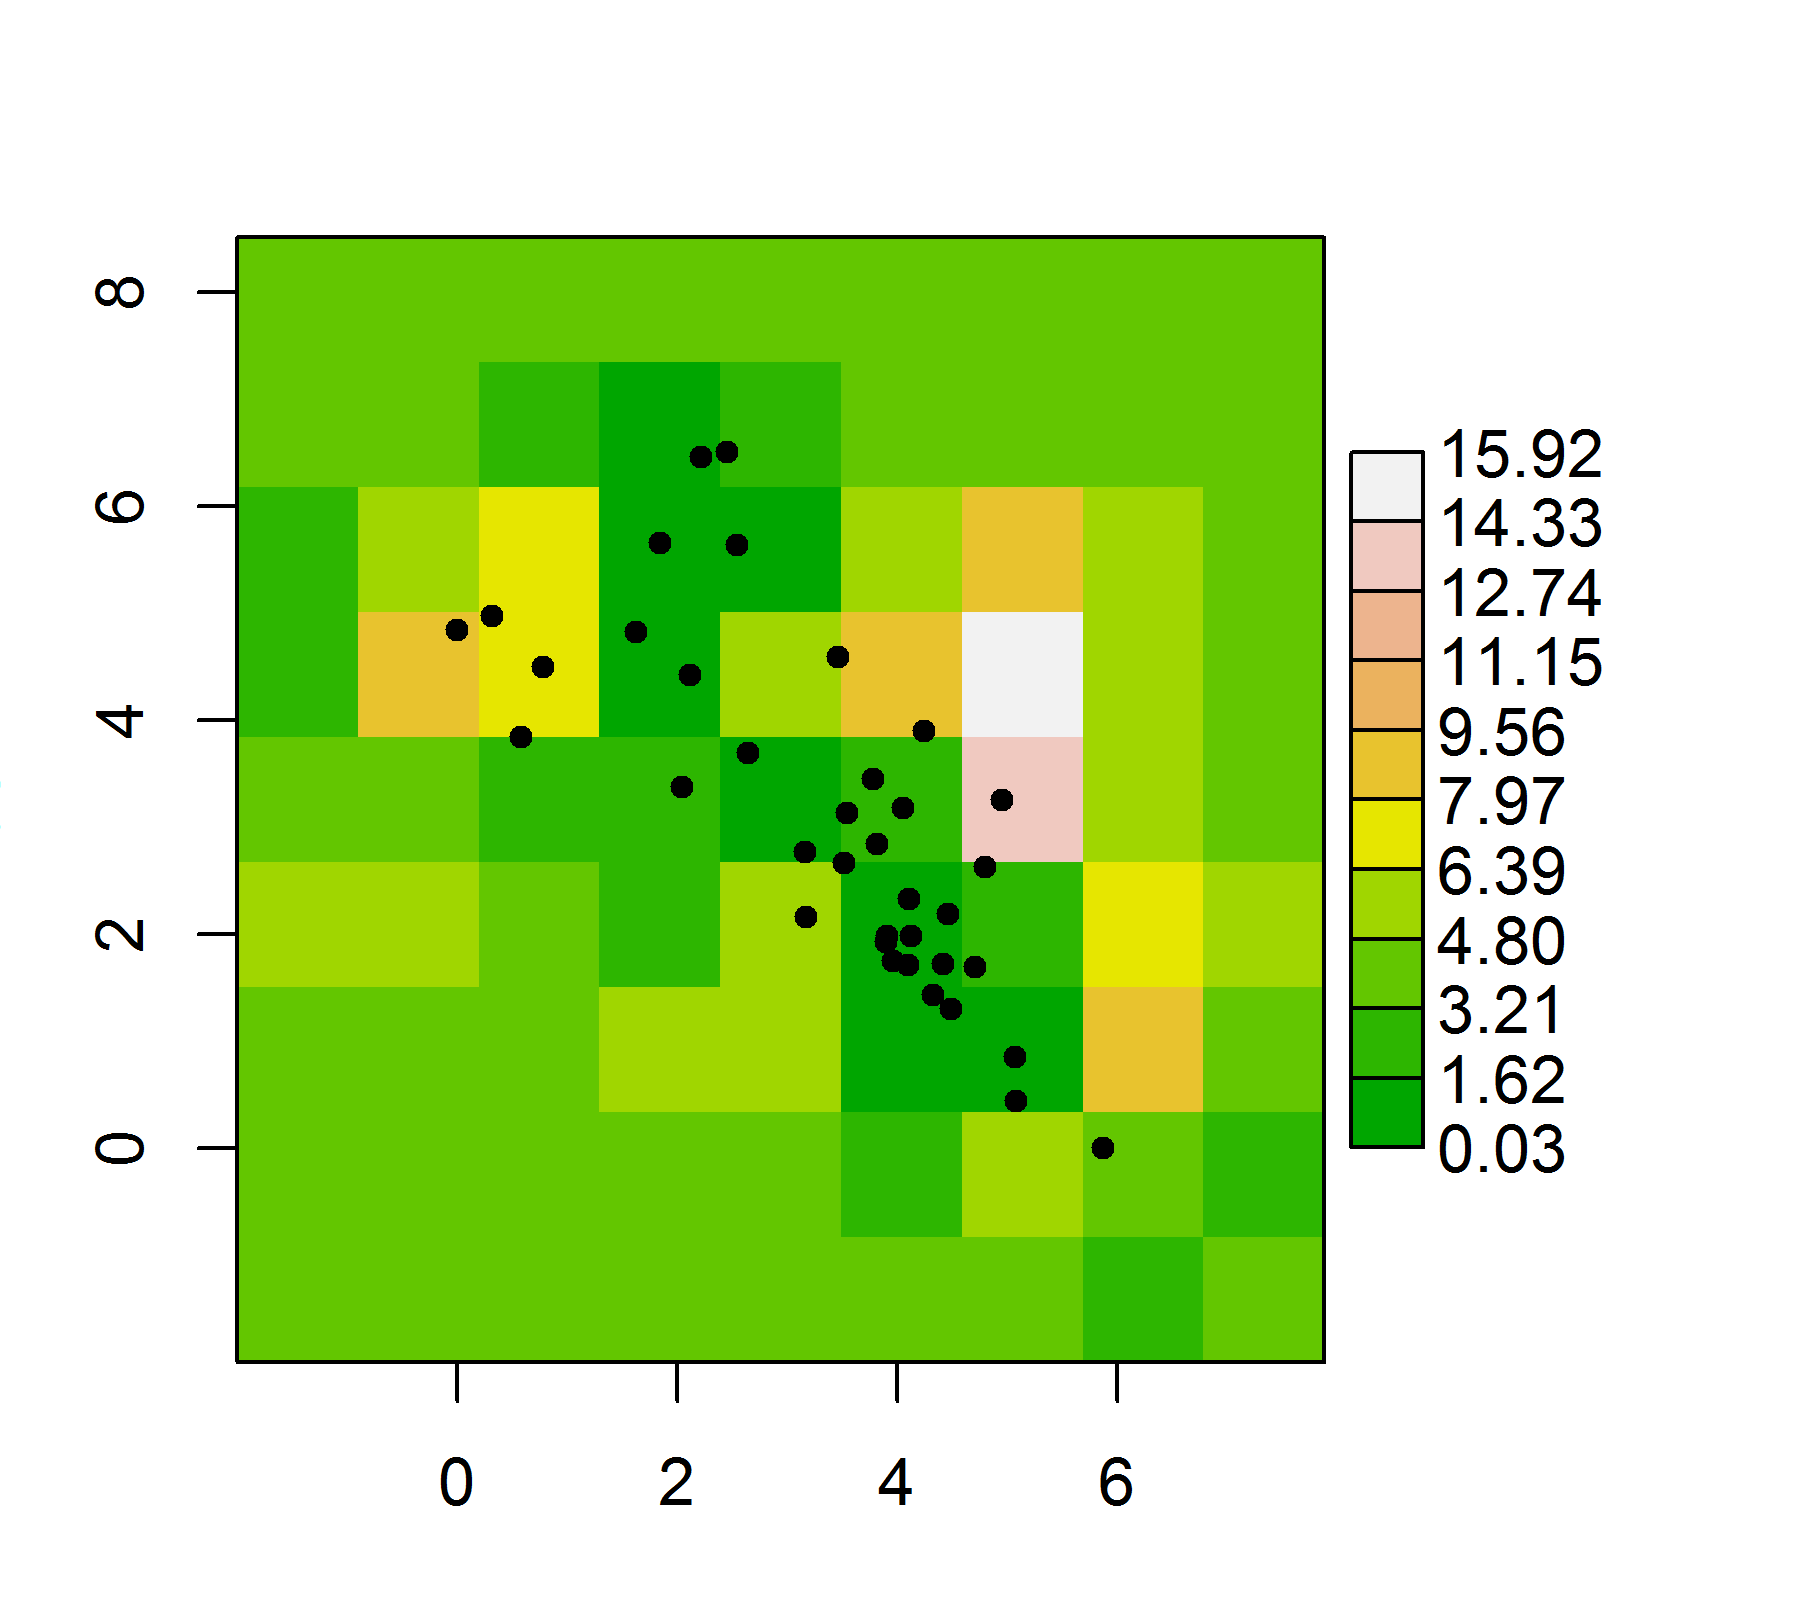
\includegraphics[height=3in,width=3.375in]{Ch4/figs/density10x10}
\end{center}
\caption{Density of wolverines (individuals per 100 $km^2$) in SE Alaska in 2007 based on
  model SCR0. Map grid cells are about 103.7 $km^2$ in area. Dots are the locations of the estimate activity centers of the XXXxxx observed individuals.}
\label{scr0.fig.density10x10}
\end{figure}

\begin{figure}
\begin{center}
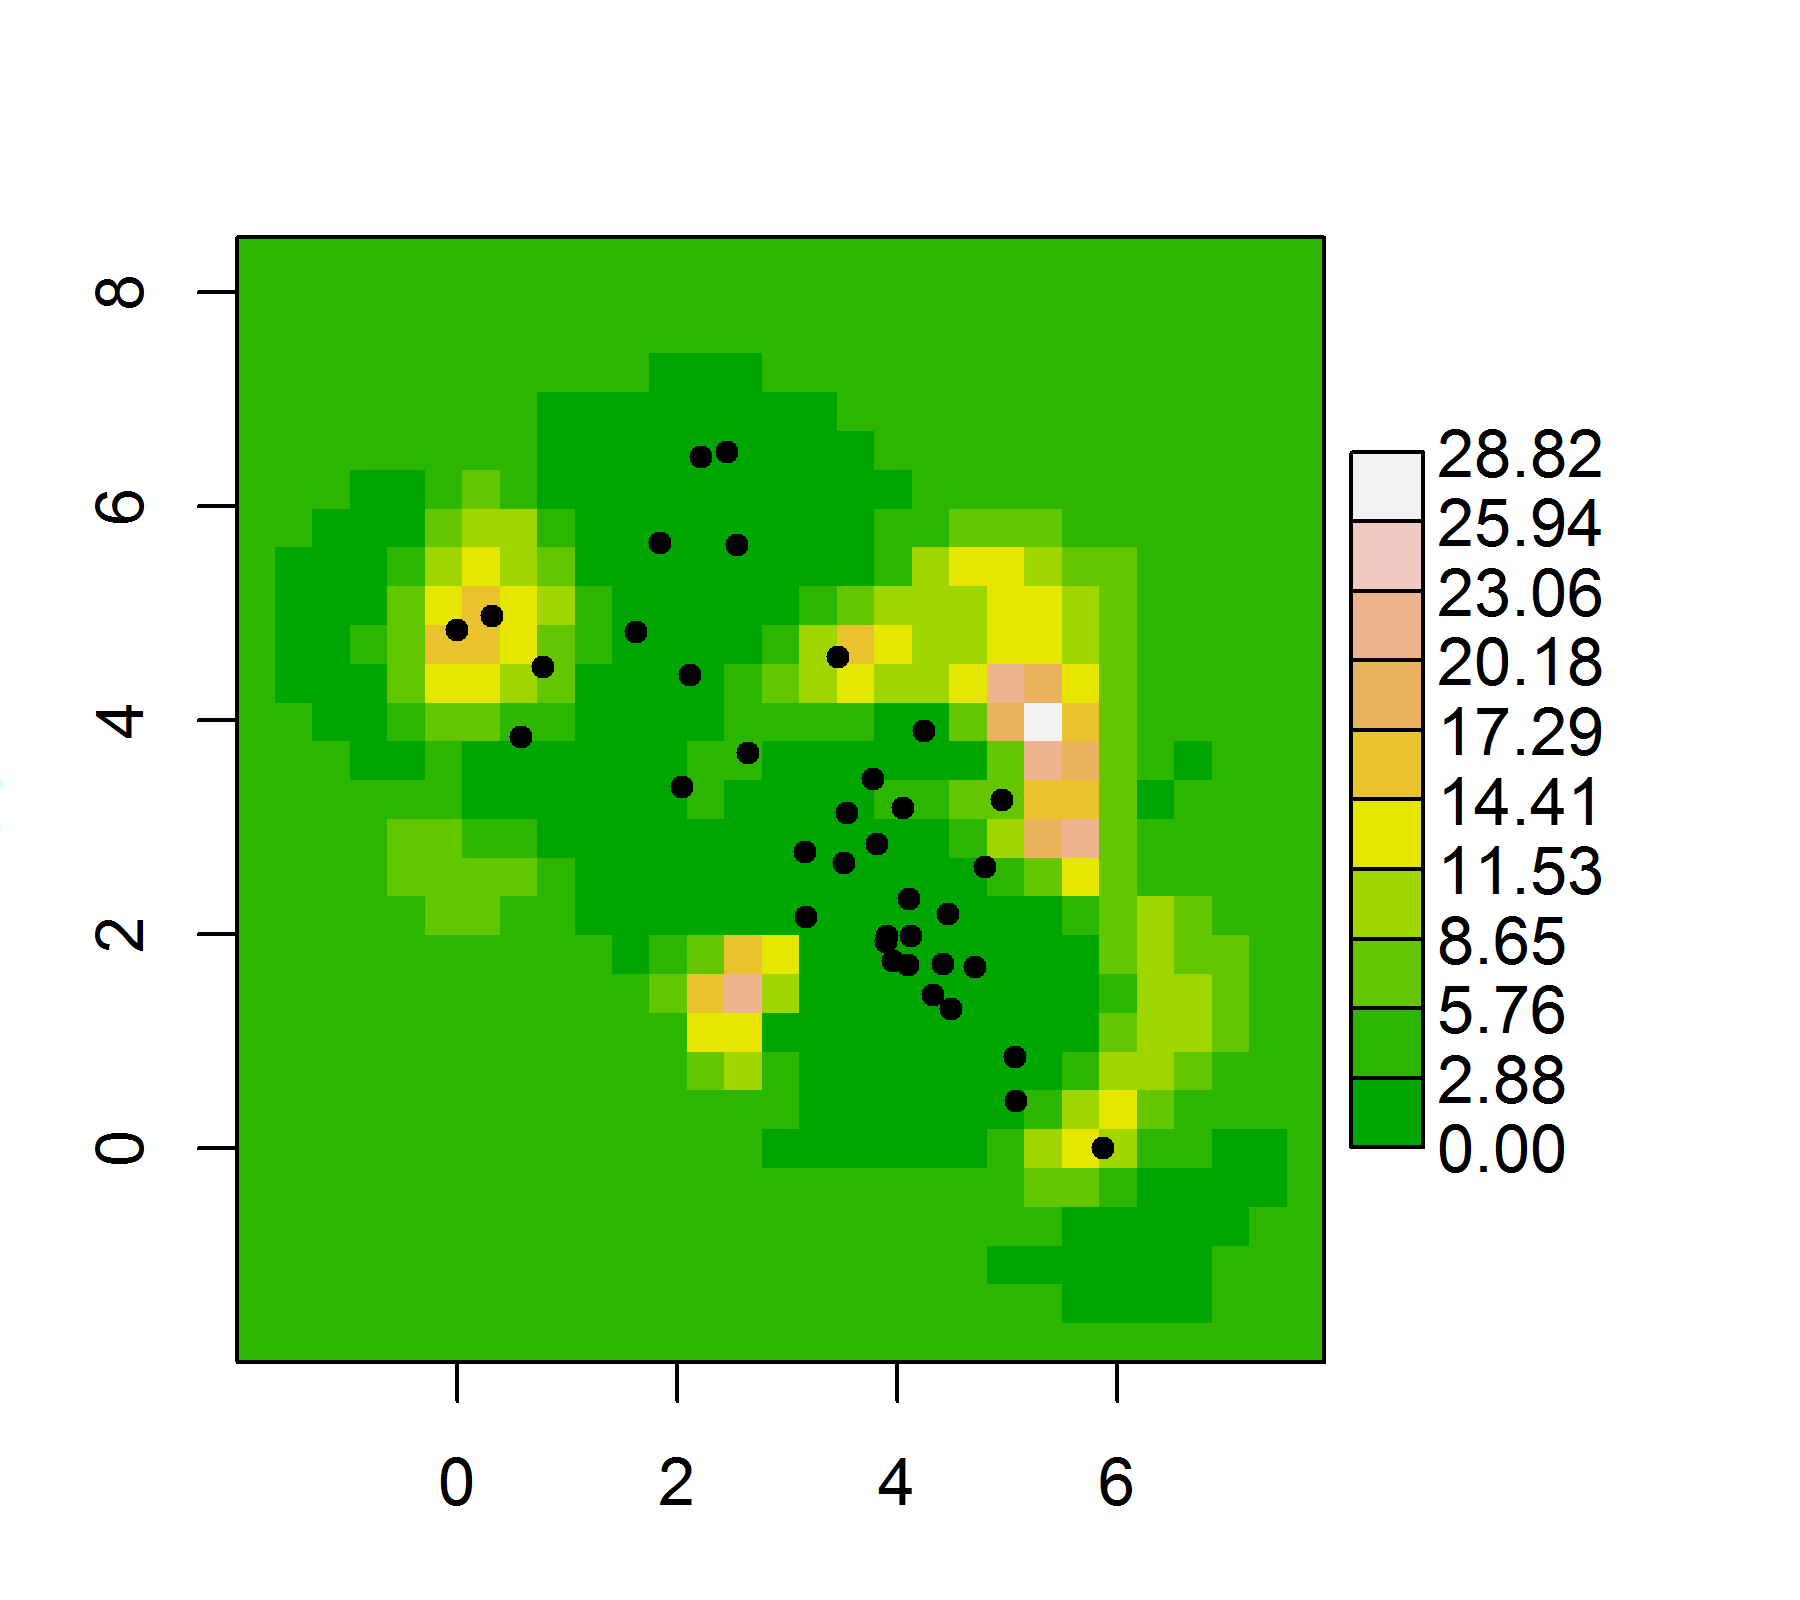
\includegraphics[height=3in,width=3.375in]{Ch4/figs/density30x30}
\end{center}
\caption{Density of wolverines (individuals per 100 $km^2$) based on
  model SCR0. Map grid cells are about 11.5 $km^2$ in area.}
\label{scr0.fig.density20x20}
\end{figure}
xxxxxx
$I would combine Fig. 4.4 and 4.5 in a single two-panel plot and call the plot ?Comparison of the effects of pixel size ...?$
$Then, I would turn color code upside down. I find it more natural to have darker mean a higher value$
$in the scale , one digit is enough$xxxxxxxxxx
xxxxx
$In Fig. 4.5., I find it funny how the estimated high-density areas are mostly away from the HR centers of the observed individuals$xxxxx

\section{Discrete State-Space}
xxxx$more informative title could be ?Allowing for unequal density in discrete state-space?$xxxx
\label{scr0.sec.discrete}

The SCR model developed previously in this chapter assumes that
individual activity centers are distributed uniformly over the
prescribed state-space. Clearly this will not always be a reasonable
assumption. In Chapt. \ref{chapt.state-space} we talk about developing models
that allow explicitly for non-uniformity of the activity centers by
modeling covariate effects on density. A simpler method of affecting
the distribution of activity centers, which we address here, is to
modify the shape and organization of the state-space explicitly. For example, we might
be able to classify the state-space into distinct blocks of habitat
and non-habitat. In that case we can remove the non-habitat from the
state-space and assume uniformity of the activity centers over the
remaining portions judged to be suitable habitat.  There are two ways
to approach this: We can use a regular grid of points to represent the
state-space, i.e., by the set of coordinates ${\bf s}_1, \ldots, {\bf
  s}_{G}$, and assign  equal probabilities to each possible value, or
we can retain the continuous formulation of the state-space but use
basic polygon operations to induce constraints on the state-space. xxxxx$what does this mean ?$xxxxxx We
focus here on the formulation of the basic SCR model in terms of a
discrete state-space but later on (Chapt. \ref{chapt.mcmc} and also
Appendix XYZ) we demonstrate the latter approach based on using
polygon operations to define an irregular state-space.

Use of a discrete state-space can be computationally expensive in {\bf
  WinBUGS}. That said, it isn't too difficult to do the MCMC
calculations in {\bf R} which we discuss briefly in Chapt.
\ref{chapt.mcmc}. The {\bf R} package {\tt SPACECAP}
\citep{gopalaswamy_etal:2011} arose from the {\bf R} implementation of the SCR model  in \citet{royle_etal:2009}.  As we will
see in Chapt. \ref{chapt.mle}, we must prescribe the state-space by a
discrete mesh of points in order to do integrated likelihood and so if
we are using a discrete state-space this can be accommodated directly
in our code for obtaining MLEs.

While clipping out non-habitat seems like a good idea, it?s not obvious
that we accomplish any biologically reasonable objective by doing
so xxxx$why not ?$xxxxx. We might prefer to do it when non-habitat represents a clear-cut
restriction on the state-space such as a reserve boundary or a lake,
ocean or river. But, 
having the capability to do this also causes people to start defining
``habitat'' vs. ``non-habitat'' based on their understanding of the
system whereas it can't be known whether the animal being studied has
the same understanding xxxxxx$I would argue that very often we do have a prett good idea of what is non-habitat$xxxxxx. Moreover, differentiating of the landscape by
habitat or habitat quality probably affects the geometry and
morphology of home ranges much more than the plausible locations of
activity centers. That is, a home range centroid could, in actual
fact, occur in a Walmart parking lot if there is pretty good habitat
around walmart, so there is probably no sense to cut out the Walmart
lot and preclude it as the location for an activity center.  It would
generally be better to include some definition of habitat quality in
the model for the detection probability \citep{royle_etal:2012ecol}
which we address in Chapt. \ref{chapt.ecoldist}.

xxxxxx$This last para doesn?t convince me somehow. I still think that when computing density, you might want to exclude non-habitat. So the guy with its homerange center right on the Walmart parking space should of course count to the estimate of N, but the parking space should be deduced from the state-space. In some way ...$xxxxxx


\subsection{Evaluation of Coarseness of Discrete Approximation}

The coarseness of the state-space should not really have much of an
effect on estimates if the grain is sufficiently fine relative to
typical animal home range sizes.  Why is this?  We have two analogies
that can help us understand this. First is the relationship to model
$M_{h}$.  As noted in sec. \ref{scr0.sec.scrmh} above, we can think
about SCR models as a type of finite mixture
\citep{norris_pollock:1996, pledger:2000} where we are fortunate to be
able to obtain direct information about which group individuals
belong to (group being location of activity center).  In the standard
finite mixture models we typically find that only 1 or a very small
number of groups (e.g., 2 or 3 at the most) can explain really high
levels of heterogeneity and are adequate for most data sets of small
to moderate sample sizes. We therefore expect a similar effect in SCR
models when we discretize the state-space.
We can also
think about discretizing the state-space as being related
to numerical integration where we find (see
Chapt. \ref{chapt.mle}) that we don't need a very fine
grid of support points to evaluate the integral to a reasonable
level of accuracy. We demonstrate this here by reanalyzing simulated
data using a state-space defined by a different numbers of support points.
We provide an {\bf R} script called \mbox{\tt SCR0bayesDss.fn} in the
{\bf R} package \mbox{\tt scrbook}.  We note that for this comparison
we generated the actual activity centers as a continuous random
variable and thus the discrete state-space is, strictly speaking, an
approximation to truth. That said, we regard all state-space
specifications as approximations to truth in the sense that they
represent a component of the SCR model.
Thus the use of any
specific discrete state-space is not intrinsically more ``wrong'' than
any specific continuous representation.

As with our {\bf R} function \mbox{\tt SCR0bayes}, the modification
\mbox{\tt SCR0bayesDss} will use either {\bf WinBUGS} or {\bf
  JAGS}. In addition, it requires a grid resolution argument
(\mbox{\tt ng}) which is the square-root of the number of points in
the state-space grid.
To execute this function we do, for example:
{\small
\begin{verbatim}
library("scrbook")
data<-simSCR0.fn(discard0=TRUE,sd=2013)   # generate data set
out1<-SCR0bayesDss(data,ng=8,M=200,engine="jags",ni=2000,nb=1000) # JAGS
out2<-SCR0bayesDss(data,ng=8,M=200,engine="winbugs",ni=2000,nb=1000) # WinBUGS
\end{verbatim}
}
We fit this model to the same simulated data set for 
$6 \times 6$, $9 \times 9$, $12 \times 12$, $15\times 15$,
$20\times 20$, $25 \times 25$ and $30 \times 30$ state-space grids.
We used 2000 burn, 12000 total iters with 3 chains, yielding a total
of 30000 posterior samples.
For {\bf WinBUGS}, which takes considerably more time (see below),
 we used 3 chains of 5k total with 1k burnin means 12k
total posterior samples.
Summary results for these analyses are shown in
Table XYZ\footnote{To finish later}.

\begin{verbatim}
Table XYZ.Effect of grid coarseness on estimates of N using JAGS and
WinBUGS.

$I would only show results from one engine. COuld simply say in the text that WB was about 5x slower$
JAGS run from rjags
             Mean       SD    NaiveSE  Time-seriesSE  runtime
6    N     109.7717 15.98959 0.0923160    0.377737    1239
9    N     114.4621 16.72025 0.0965344    0.468659    1267
12   N     115.4309 17.12403 0.098866     0.464830    1576
15   N     114.7699 17.0242  0.0982894    0.425238    1638
20   N     116.0370 17.10686 0.0987665    0.486867    1647
25   N     116.3228 16.98323 0.0980527    0.465527    1661
30   N     116.4252 17.4078  0.100504     0.533735    1806
WinBUGS run from R2WinBUGS
             Mean       SD    NaiveSE  Time-seriesSE  runtime
6    N     111.6699 16.61414 0.1516657   0.682008     2274
9    N     114.2294 17.99109 0.1642355   0.833291     4300
12   N     115.9806 17.3843  0.1586964   0.762756     7100
15   N     115.379  17.93721 0.1637436   0.832483    13010

Note: WinBUGS based on fewer samples too!
\end{verbatim}

The results in terms of the posterior summaries are, as we
expect, very similar using {\bf WinBUGS}. However, it was interesting
to note that {\bf WinBUGS} runtime is much worse (note the number of
iterations is lower for {\bf WinBUGS} yet the runtime is much longer)
and, furthermore, it seems to scale with the size of the
discrete state-space grid. While that was expected, it was unexpected
that the runtime of {\bf JAGS} would seem relatively consistent
as we increase the grid size.
We suspect that {\bf WinBUGS} is evaluating the full-conditional for
each activity center at all $G$ possible values whereas it may be that
{\bf JAGS} is evaluating the full-conditional only at a subset of
values or perhaps using previous calculations more effectively.

While this might suggest that one should always use {\bf JAGS} for
this analysis, we found in our analysis of the wolverine (next
section) that {\bf JAGS} could be extremely sensitive to starting
values, producing MCMC algorithms that sometimes simply did not work.

\subsection{Analysis of the wolverine camera trapping data}


We reanalyzed the wolverine data using discrete state-space grids with
points spaced by 2, 4 and 8 km (see in
Fig. \ref{scr0.fig.wolvgrids}). These were constructed from a 40 km
buffered state-space, and deleting the points over water
\citep[see][]{royle_etal:2011jwm}.  Our interest in doing this was to
evaluate the relative influence of grid resolution on estimated
density because the coarser grids will be more efficient from a
computational stand-point and so we would prefer to use them, but
only if there is no strong influence on estimated density.
The density estimates are only slightly different (xxxxsay in which wayxxxxx)is a bit different depending on the grid size. Also the
effectiveness of the MCMC algorithms is pretty remarkably
different. The 2km grid took 6 days to run!

\begin{figure}
\begin{center}
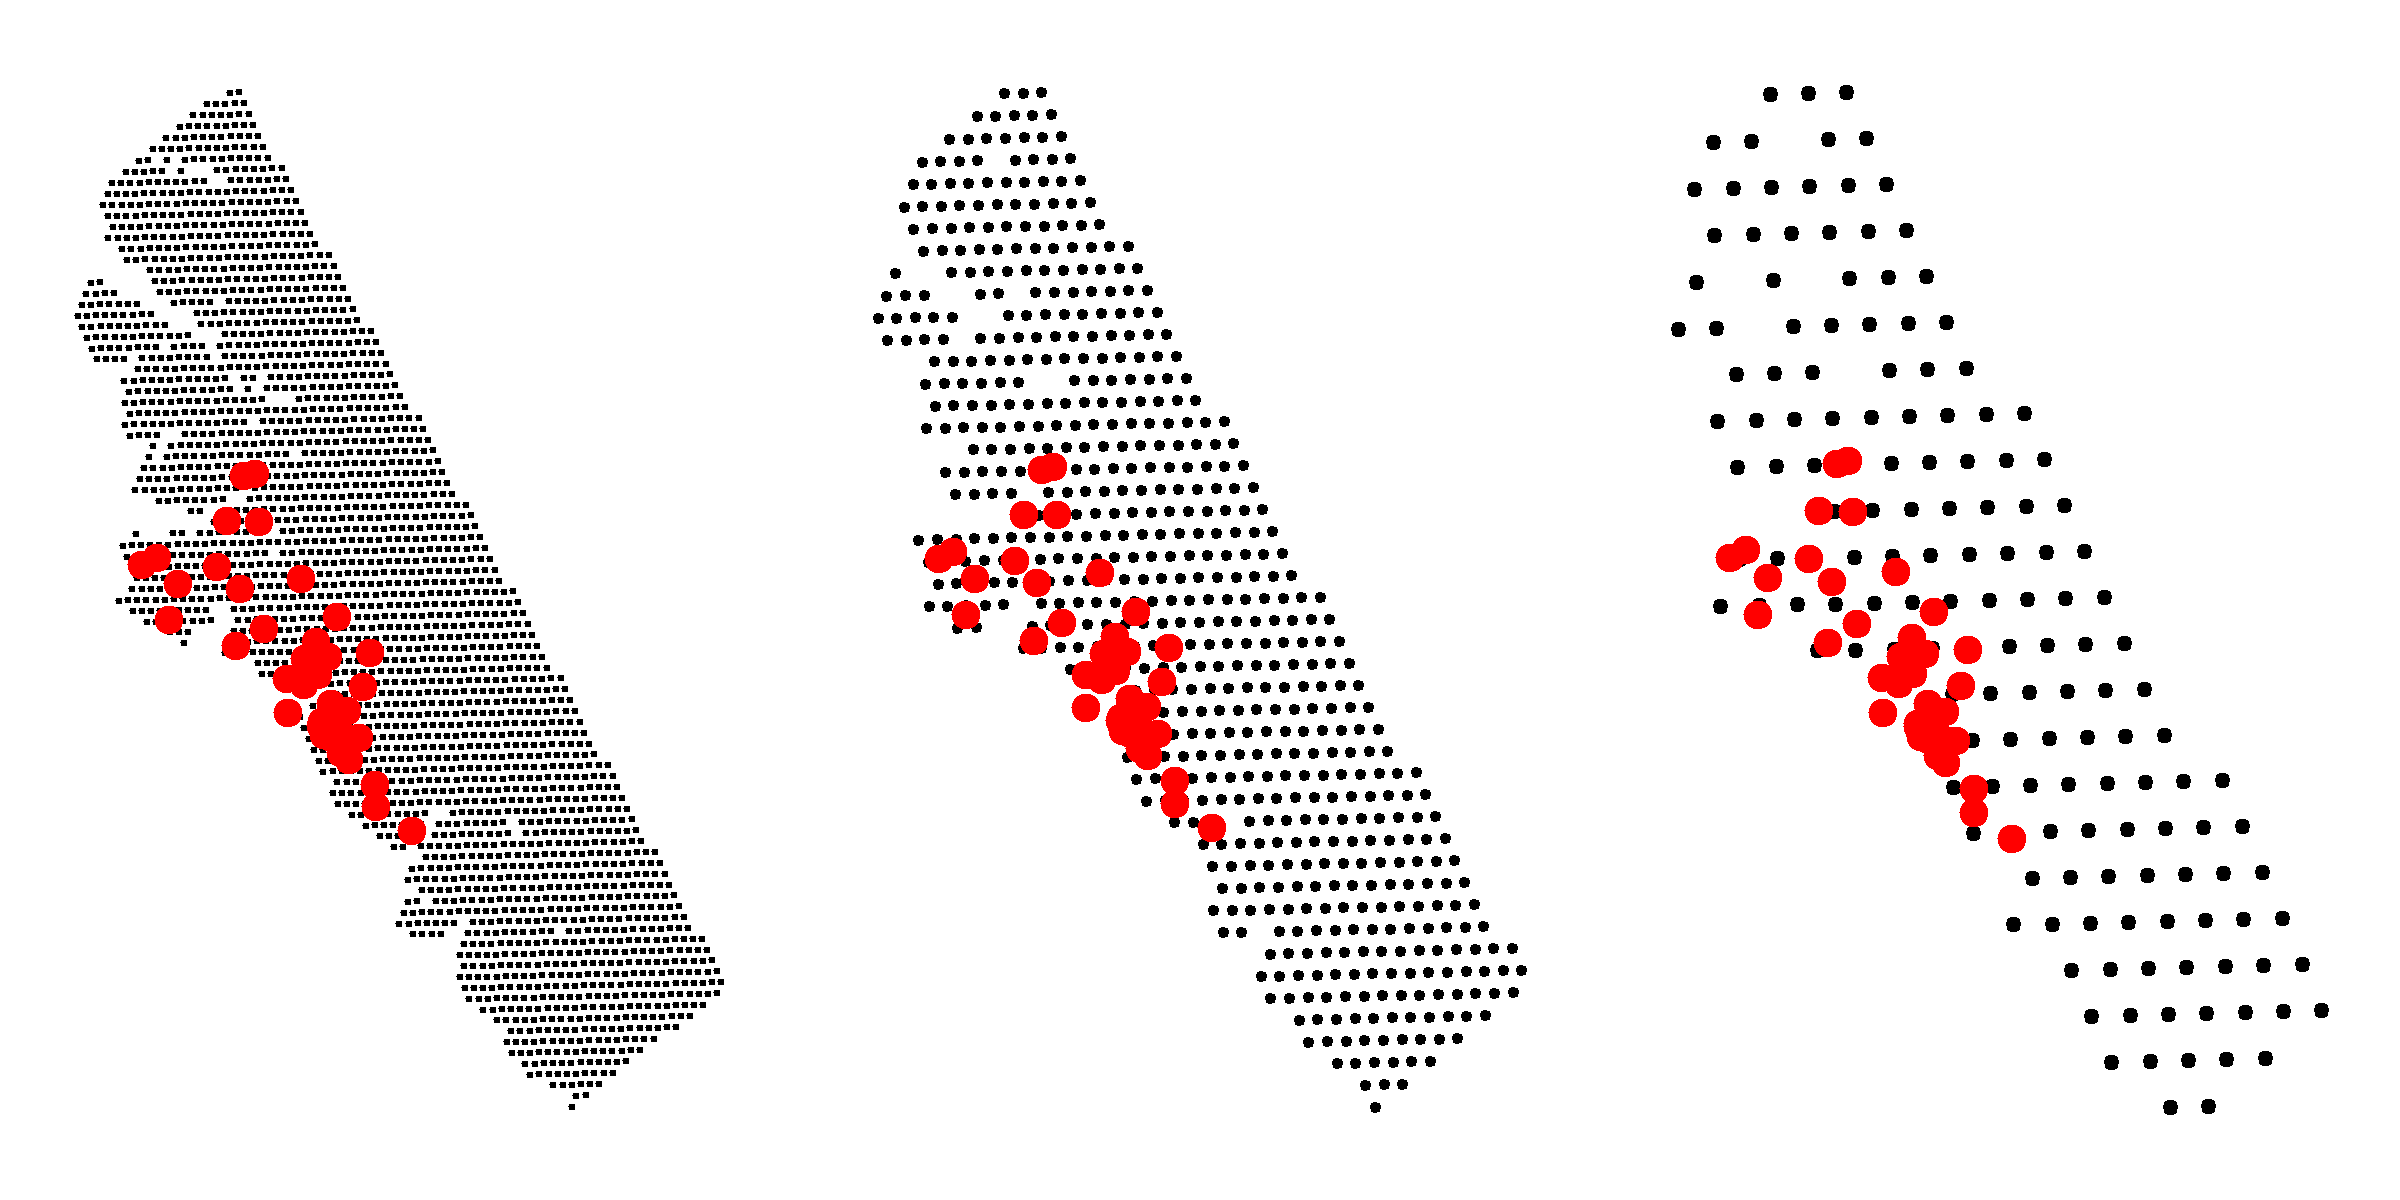
\includegraphics[height=2.5in,width=5in]{Ch4/figs/wolvgrids}
\end{center}
\caption{Comparison of the effect of pixel size on the estimated density surface of wolverine sin SE Alaska 2007. Xxxxxx 2 km 4 km and 8km wolverine state-space grids extending about
40 km from the vicinity of the trap array. }
\label{scr0.fig.wolvgrids}
\end{figure}

{\small
\begin{verbatim}
This will be summarized in a table

> print(out.2km,digits=2)
Inference for Bugs model at "modelfile.txt", fit using WinBUGS,
 3 chains, each with 11000 iterations (first 1000 discarded)
 n.sims = 30000 iterations saved
       mean    sd  2.5%   25%   50%   75%  97.5% Rhat n.eff
psi    0.43  0.09  0.27  0.37  0.43  0.49   0.63 1.00   560
sigma  0.62  0.05  0.54  0.59  0.62  0.65   0.73 1.01   160
lam0   0.05  0.01  0.04  0.04  0.05  0.06   0.07 1.01   320
p0     0.05  0.01  0.03  0.04  0.05  0.05   0.06 1.01   320
N     86.56 16.94 57.00 75.00 85.00 97.00 124.00 1.00   510
D      8.78  1.72  5.78  7.60  8.62  9.83  12.57 1.00   510

For each parameter, n.eff is a crude measure of effective sample size,
and Rhat is the potential scale reduction factor (at convergence, Rhat=1).
> print(out.4km,digits=2)
Inference for Bugs model at "modelfile.txt", fit using WinBUGS,
 3 chains, each with 11000 iterations (first 1000 discarded)
 n.sims = 30000 iterations saved
       mean    sd  2.5%   25%   50%    75%  97.5% Rhat n.eff
psi    0.45  0.09  0.28  0.38  0.44   0.50   0.64    1  1300
sigma  0.61  0.04  0.53  0.58  0.61   0.64   0.71    1  1600
lam0   0.05  0.01  0.04  0.05  0.05   0.06   0.07    1  2500
p0     0.05  0.01  0.03  0.04  0.05   0.05   0.07    1  2500
N     89.25 17.44 59.00 77.00 88.00 100.00 127.00    1  1100
D      9.01  1.76  5.96  7.77  8.88  10.10  12.82    1  1100

For each parameter, n.eff is a crude measure of effective sample size,
and Rhat is the potential scale reduction factor (at convergence, Rhat=1).
> print(out.8km,digits=2)
Inference for Bugs model at "modelfile.txt", fit using WinBUGS,
 3 chains, each with 11000 iterations (first 1000 discarded)
 n.sims = 30000 iterations saved
       mean    sd  2.5%   25%   50%   75%  97.5% Rhat n.eff
psi    0.42  0.09  0.26  0.36  0.41  0.47   0.61 1.00   940
sigma  0.68  0.05  0.59  0.64  0.67  0.71   0.77 1.01   220
lam0   0.05  0.01  0.03  0.04  0.05  0.05   0.06 1.00   560
p0     0.05  0.01  0.03  0.04  0.04  0.05   0.06 1.00   560
N     83.18 16.14 56.00 72.00 82.00 93.00 119.00 1.00   700
D      8.28  1.61  5.57  7.17  8.16  9.26  11.84 1.00   700

For each parameter, n.eff is a crude measure of effective sample size,
and Rhat is the potential scale reduction factor (at convergence, Rhat=1).
\end{verbatim}
}


\begin{comment}
We did the analysis in JAGS also. The results are shown below. {\bf Note}: I
am going to run these again but for longer to finalize the results.

{\small
\begin{verbatim}
 ### 01/10/2012 -- need to rerun these JAGS runs but use more
iterations and check results.


2km
Iterations = 7001:13000
Thinning interval = 1
Number of chains = 3
Sample size per chain = 6000

          Mean        SD  Naive SE Time-series SE
N     86.28522 16.950626 1.263e-01      0.4878973
lam0   0.04807  0.007512 5.599e-05      0.0002199
p0     0.04581  0.006820 5.083e-05      0.0001996
psi    0.28904  0.062117 4.630e-04      0.0017481
sigma  0.62769  0.043596 3.249e-04      0.0018724

4km
          Mean        SD  Naive SE Time-series SE
N     85.53139 16.998966 1.267e-01      0.5181297
lam0   0.04636  0.007542 5.621e-05      0.0002382
p0     0.04425  0.006867 5.118e-05      0.0002172
psi    0.28650  0.061922 4.615e-04      0.0018276
sigma  0.64281  0.048321 3.602e-04      0.0022911

8km
          Mean        SD  Naive SE Time-series SE
N     83.97039 16.508146 1.230e-01      0.4548782
lam0   0.04519  0.006919 5.157e-05      0.0001738
p0     0.04319  0.006319 4.710e-05      0.0001589
psi    0.28146  0.060653 4.521e-04      0.0016555
sigma  0.66956  0.040989 3.055e-04      0.0015070
\end{verbatim}
}
\end{comment}




\begin{comment}


\subsection{SCR models as multi-state models}

While we invoke a discrete state-space artificially, by gridding the
underlying continuous state-space, sometimes the state-space is more
naturally discrete. Consider a situation in which discrete patches of
habitat are searched using some method and it might be convenient (or
occur inadvertently) to associate samples to the patch level instead
of recording observation locations. In this case we might use a model
${\bf s}_{i} \sim dcat(probs[])$  where $probs[]$ are the probabilities that
an individual inhabits a particular patch. We consider such a case
study in chapter XXPoissonXXX from \citet{mollet_etal:2012} who
obtained a population size estimate of a large grouse species known as
the capracaillie. Forest patches were searched for scat which was
identified to individual by DNA analysis.
Even when space is {\it not}
naturally discrete, measurements are often made at a fairly coarse
grain (e.g., meters or tens of meters along a stream), or associated
with spatial quadrats for scat searches and therefore the state-space
may be effectively discrete in many situations.

This discrete formulation of SCR models suggests that SCR models are
related to ordinary multi-state models \citep[][ch. 9]{kery_schaub:2011}
which are also parameterized in terms of a discrete state
variable which is often defined as a spatially-indexed state related
either to location of capture or breeding location. While many
multi-state models exist in which the state variable is not related to
space, multi-state models have been extremely useful in development
models of movements among geographic states and indeed this type of
problem motivated their early developments by \citet{arnason:1972,
  arnason:1973} and \citet{hestbeck_etal:1991}.  We pursue this
connection a little bit more in chapter XXX XYZ.

\end{comment}



\section{ Summary and Outlook }

We have emphasized throughout this chapter that the basic SCR
model is an ordinary capture-recapture model for
closed populations, but augmented with a set
of latent individual effects , ${\bf s}_{i}$, which relate encounter
probability to some sense of individual location. SCR models are
therefore a type of individual covariate model (as introduced in
chapter \ref{chapt.closed}) -- but with imperfect information about the
individual covariate. In other words, they are GLMM-type of models.
 Another class of capture-recapture models
that SCR models are closely related to is the so-called ``model $M_{h}$.'' xxxxx$You do have to introduce the Otis et al. catalogue somewhere in the book, since you refer to prominently to some if its members$xxxxxx
The effect of introducing a spatial location for individuals is that
it induces heterogeneity in detection probability, as in model
$M_{h}$. However, unlike model $M_{h}$, we obtain some information
about the individual effect which is completely latent in model
$M_{h}$. If the state-space of the random effect ${\bf s}$ is discrete,
the SCR model resembles more closely the finite-mixture 
heterogeneity models \citep{norris_pollock:1996} which parameterizes
heterogeneity by assuming that individuals belong to discrete classes
or groups (e.g., having high, medium, low values of encounter probability). In the context of SCR models we
obtain some information about the group membership  in the
locations where individuals are captured.  Given the direct
relationship of SCR models with so many standard classes of models, we
find that they are really quite easy to analyze using standard MCMC
methods encased in black boxes such as {\bf WinBUGS} or {\bf JAGS} and
no doubt other packages. They are also easy to analyze using classical
likelihood methods, which we address in Chapt. \ref{chapt.mle}.

xxxxxx$In the next I find hard to understand the difference between the uniformity of the prior for the activity center locations and the non-uniformity of their posterior. What excatly is the relevance of that ? What is the difference between this and any other Bayesian analysis, where we have also usually an assumption like ?uniformity? about where something (typically a parameter value) sits and then after incorporating the information in the data, this ?space? (the posterior) is no longer uniform. Not sure whether this makes sense ... ?$ xxxxxxFormal consideration of the collection of individual locations $({\bf
  s}_{1}, \ldots, {\bf s}_{N})$ in the model is fundamental to all of
the models considered in this book. In statistical terminology, we
think of the collection of points $\{ {\bf s}_{i} \}$ as a realization of a
point process and part of the promise, and ongoing challenge, of SCR
models is to develop models that reflect interesting biological
processes, for example interactions among points or temporal dynamics
in point locations.  Here we considered the simplest possible point
process model - the points are independent and uniformly
(``randomly'') distributed over space. Despite the simplicity of this
assumption, it should suffice in many applications of SCR models
although we do address generalizations of this model in later
chapters. Moreover, even though the {\it prior} distribution on the
point locations is uniform, the realized pattern may deviate markedly
from uniformity as the observed encounter data provide information to
impart deviations from uniformity. Thus, the estimated density map
will typically appear distinctly non-uniform.  As a general rule,
information in the data will govern estimates of individual point
locations so even fairly complex patterns of non-independence or
non-uniformity will appear in the data. That is, we find in
applications of the basic SCR model that this simple {\it a priori}
model can effectively reflect or adapt to complex realizations of the
underlying point process.  For example, if individuals are highly
territorial then the data should indicate this in the form of
individuals not being encountered in the same trap - the resulting
posterior distribution of point locations should therefore reflect
non-independence.  Obviously the complexity of posterior estimates of
the point pattern will depend on the quantity of data, both number of
individuals and captures per individual.  Because the point process is
such an integral component of SCR models, the state-space of the point
process plays an important role in developing SCR models. As we tried
to emphasize in this chapter, the choice of the state-espace is part of
the model. It can have an influence on parameter estimates and other
inferences such as model selection (see chapter \ref{chapt.gof}). We
emphasize however that this is not an arbitrary decision like
``buffering'' because the model induces an explicit interpretation of
parameters and statistical effect on estimators xxxxx$what does this mean ?$xxxxxx.

We showed how to conduct Bayesian inference about the underlying point process
including calculation of density maps from posterior output. We can do
other things we normally do with spatial point processes such as
compute K-functions xxxx$need references for such things$ xxxxxxand test for ``complete spatial randomness''
(CSR) which we develop in Chapt.  \ref{chapt.gof}. 


xxxxx$I would tone down the next paragraph. Also, after having read this chapter (and understood at least the main things in it), this question does not strike me as very obvious anymore$ xxxxxAn obvious question that might be floating around in your mind is why
should we ever go through all of this trouble when we could just use
{\bf MARK} or {\bf CAPTURE} xxx$this bold face is intrusive on the eye$ xxxxxto get an estimate of $N$ and apply $1/2$
MMDM methods?  The main reason is that these conventional methods are
predicated on models that represent explicit misspecifications of both
the observation and ecological process - they are wrong!  Not just
wrong, because of course all models are wrong, but they're not even
{\it plausible} models! Thus while we might be able to show adequate
fit or whatever, we think as a conceptual and philosophical model one
should not be using models that are not even plausible data-generating
models -- even if the plausible ones don't fit!  Perhaps more
charitably, these ordinary non-spatial models are models of the wrong
system. They do not account for trap identity. They don't account for
spatial organization or ``clustering''xxx $why quotes ?$xxxx of individual encounters in
space. And, ``density'' xxxx$why quotes ? And note that density is not a parameter in SCR models either, but a derived quantity$ xxxxis not a parameter of those models because
density has no meaning absent an explicit representation of space. If
we do define space explicitly, e.g., as a buffered minimum convex
hull, then the normal models ($M_{0}$, $M_{h}$, etc..) assume that
individual capture-probability is not related to space, no matter how
we define the buffer.  Conversely, the SCR model is a model for
trap-specific encounter data - how individuals are organized in space
and interact with traps. SCR models provide a coherent framework for
inference about density or population size and also, because of the
formality of their derivation, can be extended and generalized to a
large variety of different situations, as we demonstrate in subsequent
chapters.

xxxx$General comment again: add more pertinent references, especially at places like introductions and summaries like here$xxxxxx

In the next few chapters we continue to work with this basic SCR
design and model but consider some important extensions of the basic
model.  For example, we consider
extensions
to  include covariates that vary by individual, trap, or over time
(Chapt.  \ref{chapt.covariates}), spatial covariates on density
(Chapt.  \ref{chapt.state-space}),
 open populations (Chapt. \ref{chapt.open}), model assessment and
 selection (Chapt. \ref{chapt.gof}) and other topics.
We also consider technical details of Bayesian (Chapt. 
\ref{chapt.mcmc}) and  maximum
likelihood (Chapt.  \ref{chapt.mle}) estimation so that the interested
reader can develop or extend their own methods to suit their needs.


\chapter{Other observation models}
\label{chapt.poisson}

\chapter{Maximum likelihood estimation}
\label{chapt.mle}

\chapter{MCMC details}
\label{chapt.mcmc}

\chapter{Goodness of Fit and stuff}
\label{chapt.gof}

\chapter{Covariate models}
\label{chapt.covariates}

\chapter{Inhomogeneous Point Process}
\label{chapt.ipp}

\chapter{Open models}
\label{chapt.open}


\end{comment}


\bibliography{AndyRefs_alphabetized}

\end{document}